% Created 2024-04-11 Thu 13:48
% Intended LaTeX compiler: pdflatex
\documentclass[ee,thesis]{usuthesis}

\usepackage{amsmath}                        % Cool math
\usepackage{amsfonts}                       % Cool math fonts
\usepackage{amssymb}                        % Cool math fonts
\usepackage{amsthm}                         % Lemmas, theorems, and the like
\usepackage{booktabs}                       % Used for lines in table
\usepackage{lipsum}                         % Dummy filler text
\usepackage{graphicx}                       %
\usepackage{multicol}                       % Add capability to make columns
\usepackage{multirow}                       % Add capability to make rows
\usepackage{pgfgantt}                       % Add capability to create gantt charts
\usepackage{standalone}                     % Allow standalone documents
\usepackage{subfloat}                       % Subfigures
\usepackage{tabularx}                        % Add more contol to tables
\usepackage{lscape}                         % Landscape pages
\usepackage{listings}                       % Display code
\usepackage{url}                            % Hyperlink DOI
\usepackage{doi}                            % Hyperlink DOI
\usepackage[ruled]{algorithm2e}                    % Algorithms
\usepackage{hyperref}                       %
\usepackage{subcaption}                     % Allow subfigures
\usepackage{xfp}                             % No trailing zeros
\hypersetup{colorlinks=true, linkcolor=blue,
citecolor=blue,urlcolor=blue} % Use when compiling the digital copy
% Set spacing around figures and tables to triple space
\setlength{\intextsep}{2em} % Vertical space above & below [h] floats
\setlength{\textfloatsep}{2em} % Vertical space below (above) [t] ([b]) floats
\usetikzlibrary{arrows.meta}                % Arrows for tikz
\newtheorem{definition}{Definition}[section]
\renewcommand*{\chapterautorefname}{Chapter}
\renewcommand*{\sectionautorefname}{Section}
\renewcommand*{\subsectionautorefname}{Section}
\renewcommand*{\subsubsectionautorefname}{Section}
\renewcommand*{\paragraphautorefname}{Section}
\renewcommand*{\algorithmautorefname}{Algorithm}
\newcommand{\definitionautorefname}{Definition}
\newcommand{\Or}{\textbf{ or }}
\renewcommand*{\And}{\textbf{ and }}
\newcolumntype{L}[1]{>{\hsize=#1\hsize\raggedright\arraybackslash}X}%
\newcommand\mycommfont[1]{\footnotesize\ttfamily\textcolor{gray}{#1}}
\newcommand{\T}{\mathcal{T}}                % To make it clear the difference
\newcommand{\Tau}{T}                        % between Tau and T
\newcommand{\AC}{AC(u, d, v, \eta)}            % Set the parameters for AC once
\newcommand{\PC}{PC(u, d, v)}               % Set the parameters for PC once
\newcommand{\ACi}{AC(u_i, d_i, q_i, \eta_i)}% Set the parameters for AC once
\newcommand{\PCi}{PC(u_i, d_i, q_i)}        % Set the parameters for PC once
\newcommand{\Not}{\textbf{not }}            % Custom `not' operator
\newcommand{\pvisit}{(b_i, a_i, e_i, u_i, d_i, v_i, \eta_i, \xi_i)}
\newcommand{\visit}{(b_i, a_i, e_i, u_i, d_i, q_i, \eta_i, \xi_i)}
\newcommand{\I}{\mathbb{I}}                 % Set of visit tuples
\newcommand{\C}{\mathbb{C}}                 % Charger availability information
\newcommand{\U}{\mathcal{U}}                % Uniform distribution
\newcommand{\W}{\mathcal{W}}                % Weighted distribution
\newcommand{\Sol}{\mathbb{S}}               % A shorthand for visit tuple
\newcommand{\M}{\mathbb{M}}                 % A shorthand for the metadata
\newcommand{\Hd}{\mathbb{H}}                % Set of discrete times
\newcommand{\Nu}{\mathcal{V}}               % Draw a nice Nu
\newcommand{\Iset}{I}                       % Set of visits 1-I
\newcommand{\Isetinit}{I_0}                 % Set of visits inital visits
\newcommand{\Isetfinal}{I_f}                % Set of visits final visits
\newcommand{\Bset}{B}                       % Set of visits 1-B
\newcommand{\Qset}{Q}                       % Set of visits 1-Q
\newcommand{\Jset}{J}                       % Set of visits 1-J
\newcommand{\Jsetq}{\mathbb{J}}             % Set of visits 1-J for queue active times
\newcommand{\Hset}{H}                       % Set of visits 1-H
%%-------------------------------------------------------------------------------
% Experiment parameters
\newcommand{\A}{35 }                                                            % Number of buses
\newcommand{\N}{338 }                                                           % Number of visits
\newcommand{\Cgain}{5000}                                                       % Gain applied to penalty method
\newcommand{\acharge}{0.9 }                                                     % BOD charge percentage
\newcommand{\bcharge}{0.7 }                                                     % EOD charge percentage
\newcommand{\mincharge}{25\% }                                                  % Min visit charge percent
\newcommand{\minchargeD}{0.25 }                                                 % Min visit charge decimal
\newcommand{\maxcharge}{100\% }                                                 % Max visit charge percent
\newcommand{\batsize}{388 }                                                     % Battery capacity
\newcommand{\fast}{15 }                                                         % Number of fast chargers
\newcommand{\slow}{15 }                                                         % Number of slow chargers
\newcommand{\fasts}{911 }                                                       % Speed of fast charger
\newcommand{\slows}{30 }                                                        % Speed of slow charger
\newcommand{\contvars}{7,511 }
\newcommand{\intvars}{328,282 }
\newcommand{\localcnt}{500 }                                                    % Number of local search iterations
\newcommand{\tempinit}{9000 }                                                   % Initial temperature
\newcommand{\tempcnt}{9101 }                                                    % Number of steps in temperature
\newcommand{\quicklocal}{0.25 }                                                % Time to finish local quick
\newcommand{\heuristiclocal}{0.4 }                                             % Time to finish local heuristic
%%-------------------------------------------------------------------------------
%% Solve output
%% Solve output
\newcommand{\timeran}{4.2 }                                                    % Time ran for MILP [s]
% The Committee
\majorprof{Dr. Greg Droge, Ph.D.}
\firstreader{Dr. Jacob Gunther, Ph.D.}
\secondreader{Dr. Burak Sarsilmaz, Ph.D.}

% Graduate Dean
\graddean{ D. Richard Cutler, Ph.D.}
\deantitle{ Vice Provost of Graduate Studies}

% Degree Information
\degree{Master of Science}
\month{Dec}
\gradyear{2024}
\author{Alexander Brown}
\date{}
\title{A SIMULATED ANNEALING APPROACH TO THE BATTERY ELECTRIC BUS CHARGING PROBLEM}
\begin{document}

\newtheorem*{lemma}{Lemma}

\let\ref\autoref                            % Redifine `\ref` as `\autoref` because lazy
\SetCommentSty{mycommfont}                  % Set the comment color

\preliminaries   % set frontmatter style

\maketitle

\tableofcontents
\listoftables
\listoffigures

\begin{abstract}
% A space is needed before the text starts so that the first paragraph
% is indented properly.

With an increasing adoption of Battery Electric Bus (BEB) fleets, developing a reliable charging schedule is vital to a successful migration from their fossil fuel counterparts. In this work, a BEB charging scheduling framework that considers spatiotemporal schedule constraints, fixed route schedules, fast and slow charging, and battery dynamics is modeled as a Mixed Integer Linear Program (MILP). The MILP is modeled after the Berth Allocation Problem (BAP) in a modified form known as the Position Allocation Problem (PAP). Linear battery dynamics are included to model the charging of buses while at the station. To model the BEB discharges over their respective routes, it is assumed each BEB has an average kWh charge loss while on route. The optimization coordinates BEB charging to ensure that each vehicle remains above a specified state-of-charge (SOC). The model also minimizes the total number of chargers utilized and prioritizes slow charging for battery health. The model validity is demonstrated with a set of routes and is compared to a heuristic algorithm based on charge thresholds referred to as the Qin-Modified method.

The MILP approach is then further extended via a Simulated Annealing (SA) implementation. The framework maintains the same considerations and while further developing a method to minimize the demand cost. Two generation mechanisms are implemented for the SA algorithm denoted as the ``quick'' and ``heuristic'' implementations, respectively. Similarly, the model validity is demonstrated by utilizing a set of routes sampled form the Utah Transit Authority (UTA) and comparing the results to the MILP which is utilized as a baseline as it is formulated in a way that can guarantee optimality. The Qin-Modified is again presented as another means of comparison. The results presented show that the ``heuristic'' approach was able to generate a solution comparable to that of the MILP approach over similar execution times. The SA PAP framework is further extended to incorporate non-linear battery dynamics to further increase the accuracy of the SOC model during a BEBs charging phase.
\end{abstract}
\begin{publicabstract}
% A space is needed before the text starts so that the first paragraph
% is indented properly.

With an increasing adoption of Battery Electric Bus (BEB) fleets, developing a reliable charging schedule is vital to a successful migration from their fossil fuel counterparts. In this work, a BEB charging scheduling framework that considers fixed route schedules, multiple charger types, and battery dynamics is modeled as a Mixed Integer Linear Program (MILP). The MILP is modeled after the Berth Allocation Problem (BAP) in a modified form known as the Position Allocation Problem (PAP). The optimization coordinates BEB charging to ensure that each vehicle remains above a specified charge percentage. The model also minimizes the total number of chargers utilized and prioritizes slow charging for battery health. The model validity is demonstrated with a set of routes and is compared to a heuristic algorithm based on charge thresholds referred to as the Qin-Modified method.

The MILP approach is then further extended via a Simulated Annealing (SA) implementation. The framework maintains the same considerations and while further developing a method to minimize the peak power use (demand cost). Two mechanisms are implemented for the SA algorithm denoted as the ``quick'' and ``heuristic'' implementations, respectively. The model validity is demonstrated by utilizing a set of routes sampled form the Utah Transit Authority (UTA) and comparing the results two other models: the MILP approach and the Qin-Modified. The MILP is utilized as a baseline as it is formulated in a way that can guarantee optimality. The results presented show that the ``heuristic'' approach was able to generate a solution comparable to that of the MILP over a similar execution times. The SA PAP framework is further extended to incorporate non-linear battery dynamics to further increase the accuracy of the SOC model during a BEBs charging phase.
\end{publicabstract}

\begin{dedication}
To my dearly beloved fiancée and family for all your unwavering support and encouragement over the years. May this work symbolize a token of my deepest gratitude and love in return.

%
% If you intend to have a dedication longer than one line, do not put
% it in a centering environment.  It will look better.
\end{dedication}
\begin{acknowledgments}
I wish to express my sincere gratitude to Dr. Greg Droge, my major professor, for the countless hours of reflecting, reading, encouraging, and, most of all, patience throughout the years. I thank you for the freedom that you provided to conduct my research while maintaining a guiding hand. Similarly, I wish to thank those from my committee, Dr. Jacob Gunther and Dr. Burak Sarsilmaz.
\\
\begin{flushright}
Alexander Brown
\end{flushright}
\end{acknowledgments}

\body  % set main body style

\chapter{INTRODUCTION}
\label{sec:introduction}
With an ever-increasing interest in the electrification of vehicles in the push for greener transportation, many
organizations and companies have been looking to adopt the electrification of fleet of vehicles \cite{khan-2022-inves}.
This transition is also stemming into the electrification of public bus transportation via battery power, i.e., battery
electric buses (BEBs) \cite{li-2016-batter-elect,guida-2017-zeeus-repor-europ}. In particular, agencies such as the
Utah Transit Authority (UTA), have directed focus in replacing their fleets with BEBs. Alongside all the benefits that
are associated with BEBs come new challenges that must be addressed prior to their integration into mainstream
utilization. The energy storage capacity of BEBs is typically significantly less than their combustion counterparts
while also have significantly longer refueling periods \cite{xylia-2018-role-charg,li-2016-batter-elect}. This is
further complicated due to the care that must be taken in prolonging the lifespan of the battery
\cite{lutsey-2019-updat-elect,edge-2021-lithium,millner-2010-model-lithium}. As a further complication, BEB
refueling is no longer a fixed cost (i.e. price per gallon multiplied by tank size). Utility companies, in addition to
charging for the total energy consumed over a pay period, often further introduce a demand cost. The demand cost is
based on the peak power drawn during the pay period (i.e., charging multiple BEBs simultaneously), and can significantly
impact the overall monetary cost of maintaining the BEBs. Due to these factors, the charging schedules for the BEBs
significantly impacts the overall cost of utilizing the fleet. This work introduces a scheduling framework for a
fixed-schedule fleet of BEBs that utilizes a proportional battery dynamics model, accounts for multiple charger types,
allows partial charging, and attempts to minimize the monetary cost by considering the total energy consumed by the
schedule as well as peak power use.

BEBs have been in service for many major markets, North America, Europe, and China, for more than a decade with expected
growth in the near future \cite{deng-2021-survey-elect}. The Asia Pacific market is forecasted to dominate the sales
and some major companies of the industry have also begun to enter the global market such as Volvo, BYD, and Proterra by
2025 \cite{deng-2021-survey-elect}. Much focus has been placed on the engineering of individual BEBs such as battery
type, brake regenerative charging, optimal battery charging, and battery degradation \cite{chen-2008-desig-grey,abdollahi-2016-optim-batter,kuhne-2010-elect,deng-2021-survey-elect}. The interest of route scheduling, charging
fleets, and optimizing the infrastructure are problems of more recent interest and are therefore timely and increasingly
relevant problems as EV/BEBs become more commonplace \cite{hoke-2014-accoun-lithium,sebastiani-2016-evaluat-elect,wei-2018-optim-spatio}.

Literature shows an interest in solving the problem of assigning BEBs to charging queues or optimizing their
infrastructure \cite{wei-2018-optim-spatio,sebastiani-2016-evaluat-elect,hoke-2014-accoun-lithium,wang-2017-elect-vehic}. In fact, many works attempt to solve both problems simultaneously
barring some simplification whether it be only allowing chargers of a single type
\cite{he-2020-optim-charg,tang-2019-robus-sched}. If multiple chargers are used, then one of each type is assigned at
each location. Others have also assumed that a BEB shall recieve full charge upon each arrival
\cite{wei-2018-optim-spatio,wang-2017-elect-vehic,zhou-2020-bi-objec,wang-2017-optim-rechar}. Some works on the
stochastic effects of energy consumption while on route for a BEB as well as trip times \cite{zhou-2020-collab-optim,bie-2021-optim-elect}. One other source, as far as the research for this work has shown, describes a method of
producing a BEB charge schedule wih a high fidelity while accounting for multiple charger times as well as being able to
minimize over the total charger count \cite{whitaker-2023-a-network}.

The work described in this thesis is similar to the work in \cite{whitaker-2023-a-network}; however provides an
alternate method of modeling the problem in what is known as the Position Allocation Problem (PAP). The PAP is modeled
after the Berth Allocation Problem (BAP), which was designed to optimally schedule cargo vessels to be berthed and
serviced \cite{buhrkal-2011-model-discr,imai-2001-dynam-berth,frojan-2015-contin-berth}. The PAP utilizes this
notion to develop a model of assigning EVs to queue in ordered to be charged \cite{qarebagh-2019-optim-sched}.

Because the PAP's modeling is similar to that of the BAP, literature from the BAP provides a foundation for the
development of the PAP in this work. The BAP has been studied in literature since the 1990s and provides a depth of work
to derive from \cite{rodrigues-2022-berth}. The work to be introduced promises much potential for further research and
development in regard to scheduling BEBs. What follows is a Simulated Annealing (SA) implementation and extension of the
PAP utilizing Mixed Integer Linear Programming (MILP) constraints with non-linear battery dynamics.

The work proceeds as follows: \ref{sec:background-and-related-work} provides the state-of-the-art along with various
introductory material pertinent to this work. \ref{sec:milp-pap} constructs the MILP for BEB scheduling, including
modifications to the PAP queuing constraints and the development of a dynamic charging model. An example this presented
as a demonstration of the model's utility. The results are subsequently provided and discussed. In \ref{sec:sa-pap}, the
previously derived BEB charging model is adapted for a Simulated Annealing (SA) implementation. This method maintains
the same considerations from the MILP implementation, but further accounts for a peak power demand cost. An example is
then provided with discussion on the results. \ref{sec:nonlinear-battery-dynamics} further adapts the SA approach by deriving
and incorporating non-linear battery dynamics. The example from \ref{sec:sa-pap} is run again utilizing the non-linear
battery dynamics. The results are then presented and discussed.
\chapter{BACKGROUND AND RELATED WORK}
\label{sec:background-and-related-work}
The BEB queue scheduling problem is one that has been of increasing interest and relevancy in the EV/BEB industry. It is
thus important to address the state of the art by introducing relevant problems in BEB queue scheduling, which will be
addressed first. A detailed problem description shall then be presented to provide a basis of understanding of the
proposition. Relevant introductory theory will be presented throughout.

\section{State Of The Art of Battery Electric Bus Charging}
\label{sec:state-of-the-art}
Works concerning charge planning often use a version of the vehicle scheduling problem \cite{zhang-2021-optim-elect,duan-2021-refor-mixed,rinaldi-2020-mixed-fleet,tang-2019-robus-sched,li-2014-trans-bus,he-2020-optim-charg},
while others have based their implementation on alternative methods
\cite{qarebagh-2019-optim-sched,whitaker-2023-a-network}. \cite{whitaker-2023-a-network} utilizes a network flow
approach to model the scheduling while \cite{qarebagh-2019-optim-sched} utilizes what is known as the Position
Allocation Problem (PAP). Nearly all the literature reviewed considered consumption costs \cite{jahic-2019-preem,frendo-2021-open-sourc,qin-2016-numer-analy,zhou-2020-bi-objec,duan-2021-refor-mixed,mortensen-2023-cost-minim,zhou-2020-collab-optim,rinaldi-2020-mixed-fleet,zhou-2020-collab-optim}, while fewer consider demand costs
\cite{jahic-2019-preem,frendo-2021-open-sourc,qin-2016-numer-analy,mortensen-2023-cost-minim,he-2020-optim-charg}. Many of these works introduce simplifying assumptions for the sake of computation. For example,
some approaches only consider fast chargers during planing \cite{zhou-2020-collab-optim,li-2014-trans-bus,wang-2017-optim-rechar,sebastiani-2016-evaluat-elect,wei-2018-optim-spatio}. Approaches that consider more than one
charger type typically isolate the specific charger types in different locations \cite{tang-2019-robus-sched,he-2020-optim-charg}.

Variants of this problem address infrastructure as well as determining existing buses that should be replaced by a BEB
\cite{zhou-2020-bi-objec,duan-2021-refor-mixed,rinaldi-2020-mixed-fleet,zhou-2020-collab-optim}. Other works
introduce a directed graph approach to model the flow of BEBs \cite{whitaker-2023-a-network,liu-2020-batter-elect},
where this concept was expanded to simultaneously accounting for multiple charger types, partial charging, non-linear
battery charge profiles \cite{whitaker-2023-a-network}. The directed graph approach provides an easy method of modeling
the scheduling by discretizing the time horizon to \(n_Q\) sets of nodes. The nodes represent the chargers availability
and can have a maximum of one bus at a time. The buses can flow into a node to be charged and then later can exit
allowing a new bus to enter. Another method similar to the directed graph that fits the modeling of the BEB charging
scenario is the PAP \cite{qarebagh-2019-optim-sched}. The PAP is derived from the BAP which takes an input of vessel
arrival times and outputs the selection of the berthing quay. The PAP utilizes this model and redefines its inputs to EV
arrival times and outputs queues for the EVs to be charged. While the visits remain as discrete events, the time that
the BEB is on the charger is modeled in continuous time similar to \cite{frojan-2015-contin-berth,qarebagh-2019-optim-sched,zhou-2020-collab-optim}. Due to the close relationship between the BAP and PAP, BAP
literature may be used for the PAP. The literature shows methods of handling multiple quays (sets of chargers) to handle
general berthing scenarios \cite{frojan-2015-contin-berth,dai-2008-suppl-chain-analy}. Heuristic procedures for
quicker solve times have also been introduced \cite{imai-2001-dynam-berth}. Methods of defining static (full-time
horizon) and dynamic (rolling-time horizon) models have been created for daily and real-time solutions, respectively,
and even fuzzy set theory has been applied to allow for more flexible schedules \cite{bello-2019-fuzzy-activ}.

Others have assumed that BEBs always charge to full capacity \cite{duan-2021-refor-mixed,zhang-2021-optim-elect,zhou-2020-bi-objec,wang-2017-elect-vehic}, partial charging utilizing a linear battery dynamics model
\cite{wei-2018-optim-spatio,he-2020-optim-charg,mortensen-2023-cost-minim}, or non-linear battery dynamics with
partial charging \cite{whitaker-2023-a-network,zhang-2021-optim-elect,qin-2016-numer-analy,jahic-2019-preem,frendo-2021-open-sourc}. Works that assumed scheduled BEBs always charge to full capacity significantly simplify the
scheduling problem, but eliminates the key factor in reducing the demand cost, partial charging
\cite{tang-2019-robus-sched,duan-2021-refor-mixed,rinaldi-2020-mixed-fleet,zhou-2020-collab-optim}. The
approaches that utilized non-linear charging profiles with partial charging are able to achieve a reduction in the
demand cost, with the added benefit of a higher fidelity at the expense of computation \cite{zhang-2021-optim-elect}.
Exceptions to this are \cite{he-2020-optim-charg} that utilize a piecewise-linear charging profiles. This model has the
drawback of assuming that a charger is always available. A common way to model the non-linear battery dynamics is
utilizing Constant Voltage (CV), Constant Current (CC), and Constant Current Constant Voltage (CCCV)
\cite{abdollahi-2016-optim-batter,chen-2008-desig-grey}. A novel method of modeling the non-linear behavior present
in \cite{whitaker-2023-a-network} proposes a discrete linear time-invariant dynamic model that results in an
exponential decay non-linear charge profile.

The selected model for the battery charge dynamics, although pertinent to this work as it directly affects the quality
of the produced schedule, does not impact the considerations of battery health. Battery health begins to be of concern
when over-charging, under-charging, or forcing the battery to perform ``deep'' cycles \cite{zhou-2020-bi-objec,millner-2010-model-lithium,edge-2021-lithium}. Furthermore, other works have suggested that charging a battery nearly
to capacity is detrimental to the health and can significantly reduce the total charge cycles a battery may undergo
\cite{edge-2021-lithium,millner-2010-model-lithium}. While the charge profile for batteries are inherently
non-linear, some works have assumed proportional charging as linear battery dynamics remain a valid assumption when the
battery SOC is below 80\% \cite{liu-2020-batter-elect}. Thus, while linear dynamics may lack the fidelity of accuracy
above 80\%, it is able to accurately estimate the SOC within a range that will guarantee battery health. This work
begins with an implementation of linear battery dynamics then incorporates a non-linear model suggested by \cite{whitaker-2023-a-network}.

\section{Problem Description}
\label{sec:problem-description}
The work of this thesis builds upon the Position Allocation Problem (PAP) \cite{qarebagh-2019-optim-sched}, a
modification of the well studied Berth Allocation Problem (BAP), as a means to schedule the charging of electric
vehicles (EVs) \cite{buhrkal-2011-model-discr,frojan-2015-contin-berth,imai-2001-dynam-berth}. The goal of the PAP is
to allocate incoming EVs into queues to be charged as depicted in \autoref{subfig:papexample}. An example of a standard
PAP/BAP solution (their visual representations are interchangeable) is visualized in \autoref{fig:bap}, note that the
figure utilized BAP terminology. The x and y-axis represent time and queuing space, respectively. The figure discretizes
the queuing space, but it may be continuous if desired. The shaded rectangles' widths represent their respective
allocated charge times, and their heights represent the physical space taken by each EV.

\begin{subfigures}
    %%~~~~~~~~~~~~~~~~~~~~~~~~~~~~~~~~~~~~~~~~~~~~~~~~~~~~~~~~~~~~~~~~~~~~~~~~~~~~
    % BAP
    \begin{figure}[htpb]
    \centering
        \includestandalone{sup-doc/milp-pap-paper-frontiers/img/bap}
        \caption{Example of berth allocation. Vessels are docked in berth locations (horizontal) and are queued over
          time (vertical). The vertical arrow represents the movement direction of queued vessels and the horizontal
          arrow represents the direction of departure.}
        \label{subfig:bapexample}
    \end{figure}
    \hfill

    %%~~~~~~~~~~~~~~~~~~~~~~~~~~~~~~~~~~~~~~~~~~~~~~~~~~~~~~~~~~~~~~~~~~~~~~~~~~~~
    % PAP
    \begin{figure}[htpb]
    \centering
        \includestandalone{sup-doc/milp-pap-paper-frontiers/img/pap}
        \caption{Example of position allocation. Vehicles are placed in queues to be charged and move in the direction
          indicated by the arrow.}
        \label{subfig:papexample}
    \end{figure}
\end{subfigures}

Adapting the PAP model for BEBs, consider a fleet of BEBs scheduled to perform a set of prescribed routes on a given
day. An individual BEB from said fleet begins and completes an individual route at the same station from which it also
receives its charge. During each route, the BEB's State of Charge (SOC) is depleted by a certain amount. The charge
supplied during its visit must be enough to sustain the BEB's SOC at an appropriate level so that it may complete its
next route. The charge may be supplied from any single charger given a set of chargers at the station. Let the term
``arrival'' describe the time at which a BEB reaches the station. Furthermore, let the term ``visit'' denote a BEB having
arrived, awaited its predetermined time (whether it has received a charge or not), and departed from the station. Each
BEB may have multiple visits to the station throughout their working day. This paper describes a method to optimize the
assignment of each visit to a charger given a schedule for a fleet of BEBs that follow the behavior described above. The
various models presented in this work optimizes over peak power usage and energy consumption, as well as attempts to
optimize the amount of chargers utilized. Both linear and non-linear battery dynamics are introduced and implemented.

\section{Mixed Integer Linear Programming}
\label{sec:org6ec8877}

A mixed integer linear programming (MILP) problem is a class of constrained optimization in which one seeks to find a
set of continuous or integer values that maximizes or minimizes an objective function while satisfying a set of
constraints \cite{chen-2010-applied}. Given an objective function \(J\), decision variables (i.e. variables of
optimization) \(x_j \in \mathbb{R}\) and \(y_k \in \mathbb{Z}^+\), and input parameters \(c_j, d_k, a_{ij}, g_{ik}, b_i \in \mathbb{R}\), a MILP has a
mathematical structure represented as shown in \ref{eq:milp-structure} \cite{chen-2010-applied}

\begin{subequations}
\label{eq:milp-structure}
\begin{align}
&\text{max}        &J = \sum_j c_j x_j + \sum_k d_k y_k&         &               &\label{eq:fuzzy-milp-objective}\\
&\text{subject to} &\sum_j a_{ij} x_j + \sum_k g_{ik} y_k \le b_i&  &(i = 1,2,...,m)& \label{eq:fuzzy-milp-constraint}\\
&                  &x_j \ge 0&                              &(j = 1,2,...,n)& \label{eq:fuzzy-milp-continuous}\\
&                  &y_k \in \mathbb{Z^+}&                   &(k = 1,2,...,n)& \label{eq:fuzzy-milp-integer}\\
&\end{align}
\end{subequations}

The objective function in \ref{eq:fuzzy-milp-objective} comprises two parts, the continuous part, \(\sum_j c_j x_j\), and
integer part, \(\sum_k d_k y_k\). The decision variable of the first part, \(x_j\), is continuous whereas the decision variable
of the second, \(y_j\), is integer. Their respective input parameters may be integer or continuous, in the case of this
example they are modeled as continuous. The objective function's utility is to provide a numerical score to a system
(provided that a set of decision variables and input parameters are defined). While an individual score may not have any
intrinsic meaning, it provides a method of ranking different solutions of the same model. The constraint equations
(\ref{eq:fuzzy-milp-constraint} - \ref{eq:fuzzy-milp-integer}) must all be satisfied for the output of an objective

\section{Overview of the BAP}
\label{sec:overview-of-the-bap}
%% Rectangle packing figure
\begin{figure}
  \centering
  \includegraphics{sup-doc/milp-pap-paper-frontiers/img/spatiotemporal-packing}
  \caption{Example of rectangle packing problem. The large square represented by $O$ indicates the canstrained area that the set of shaded rectangles $\mathbb{O}$ must be placed within.}
  \label{fig:packexample}
\end{figure}

%% BAP/PAP solution plot example
\begin{figure}
  \centering
  \includegraphics{sup-doc/milp-pap-paper-frontiers/img/baprep}
  \caption{The representation of the berth-time space. The x and y-axis represent time and space, respectively. Along the y-axis, the dashed lines represent discrete berthing locations. These locations may be chosen to be continuous. The shaded rectangles represent scheduled vessels to be serviced. The height of each shaded rectangle represents the space taken on the berth and the width being the time to service said vessel. The vertical dashed lines are associated with vessel D and represent the arrival time, berthing time, serviced completion time, and departure time. Note that the arrival time may be before the berthing time and the completion time may before the departure time.}
  \label{fig:bap}
\end{figure}

The BAP is a rectangle packing problem where a set of rectangles, \(\mathbb{O}\), are attempted to be optimally placed in
a larger rectangle, \(O\), as shown in \autoref{fig:packexample}. The rectangle packing problem is an NP-hard problem that
can be used to describe many real-life problems \cite{bruin-2013-rectan-packin,murata-1995-rectan}. In some of these
problems, the dimensions of \(\mathbb{O}\) are held constant such as in the problem of packing modules on a chip, where
the widths and height of the rectangles represent the physical width and heights of the modules
\cite{murata-1995-rectan}. Other problems, such as the one presented in this work, allow either the horizontal or
vertical edge of each rectangle in \(\mathbb{O}\) to vary. As an example, suppose the vessel lengths are predefined
(vertical edges are static), but the service time is allowed to vary (horizontal edges are dynamic).
\cite{buhrkal-2011-model-discr}.

The BAP solves the problem of optimally assigning incoming vessels to berth positions to be serviced as shown in
\autoref{subfig:bapexample}. To relate to the rectangle packing problem, the width and height of \(O\) represent the time
horizon \(T\) seconds and the berth length \(L\) meters, respectively. Similarly, the widths and heights of each element in
\(\mathbb{O}\) represent the time spent to service vessel \(i\) and the space taken by docking vessel \(i\), respectively. In
the BAP, the vessel characteristics (length of the vessel, arrival time, handling time, desired departure time) are
assumed to be known for all vessels. A representation of a BAP solution is shown in \autoref{fig:bap}. The x and y-axis
represent time horizon and berthing space, respectively. The gray squares, labeled A, B, C, and D, represent berthed
vessels. The width of the boxes represents the time spent being serviced, and the height represents the amount of space
the vessel requires on the berth. The vertical line adjacent to ``Arrival Time'' represents the actual time that the
vessel arrives and is available to be berthed. ``Berthing Time'' is the time the vessel is berthed and begins being
serviced. ``Completion time'' represents the time at which the berthing space becomes available again.

\section{Overview of the PAP}
\label{sec:overview-of-the-pap}
The BAP defines the foundation of the PAP; however, there are some differences in the way the variables are interpreted. For
the \(i^{th}\) visit, starting service time is now the starting charge time, the berth location is now the charger queue
for assignment, and the service time is now the elapsed charge time. There are also a few clarifying concepts about how
the system is modeled. The PAP models the set of chargers as one continuous line; that is, the natural behavior of the
PAP model is to allow vehicles to be queued anywhere along the ``charge strip'' \([0,S]\). Similarly, the charge times are
continuous and can be placed anywhere on the time horizon, \([0,T]\), as long as the allocated times do not interfere with
other scheduled charge times.

\subsubsection{The PAP Formulation}
\label{sec:the-pap-formulation}
The BAP forms the basis of the PAP; however, there are some differences in the way the variables are interpreted. The
starting service time, \(u_i\) seconds, is viewed as the initial charge time, and the service time, total elapsed time
spent on the charger. Similarly, for the spatial term, \(v_i \in [0,L]\), the berth location is instead interpreted as the
initial position on the charger. There are also a few clarifying concepts about how the system is modeled. The PAP
models the set of chargers as one continuous line; that is, the natural behavior of the PAP model is to allow vehicles
to be queued anywhere along \([0,L]\). Similarly, the charge times are continuous and can be placed anywhere on the time
horizon, \([0,T]\), as long as the allocated times do not interfere with other scheduled charge times.

The PAP formulation's parameters can be divided into two categories: input parameters and decision variables. Each type
will now be introduced in turn. The following parameters are assumed to be known inputs for the MILP. \(L\) defines the
length of the charger in meters. As stated previously, it is modeled as a continuous bar meaninng that a vehicle can be
placed anywhere in the range \([0,L]\). It is assumed that the time horizon, \(T\) seconds, is known so that vehicles may be
placed temporarily in the range \([0,T]\). The total number of visits to the station over the time horizon is represented
by \(n_V\). The arrival time for each visit is represented by \(a_i\) seconds, and the required charge time is represented
by \(s_i\) seconds. The width of vehicle \(i\) is represented by \(l_i\) meters.

The decision variables provide the means by which the solver may optimize the problem. The initial and final charge
times for vehicle \(i\) are \(u_i\) and \(d_i\) seconds, respectively. The starting position on the charger is denoted as \(v_i
\in [0,L]\) meters. The temporal ordering of vehicles \(i\) and \(j\) is determined by \(\sigma_{ij} \in \{0, 1\}\), where \(\sigma_{ij} = 1
\implies\) \(i\) arrives before \(j\) for all \(1 \le i,j \le n_V\). Similarly, \(\psi_{ij} \in \{0, 1\}\) determines the relative
position of vehicles \(i\) and \(j\) on the charger: \(\psi_{ij} = 1 \implies v_i < v_j\) for all \(1 \le i,j \le n_V\).

To determine the values for each of these decision variables, a MILP was formulated in
\cite{qarebagh-2019-optim-sched}. The formulation is shown in its entirety for completeness.
The problem to be solved is

\begin{equation}
	\label{eq:bapobjective}
	\min\; \sum_{i=1}^N (d_i - a_i)
\end{equation}

Subject to:
\begin{subequations}
\label{eq:bapconstrs}
\begin{align}
    u_j - u_i - s_i - (\sigma_{ij} - 1)T \geq 0   \label{subeq:baptime}          \\
    v_j - v_i - l_i - (\psi_{ij} - 1)L \geq 0   \label{subeq:bapspace}           \\
    \sigma_{ij} + \sigma_{ji} + \psi_{ij} + \psi_{ji} \geq 1 \label{subeq:bapvalid_pos}     \\
    \sigma_{ij} + \sigma_{ji} \leq 1                   \label{subeq:bapsigma}        \\
    \psi_{ij} + \psi_{ji} \leq 1                   \label{subeq:bapdelta}        \\
    s_i + u_i = d_i                       \label{subeq:bapdetach}       \\
    a_i \leq u_i \leq (T - s_i)                 \label{subeq:bapvalid_starts} \\
    \sigma_{ij} \in \{0,1\},\;\psi_{ij} \in \{0,1\}\; \label{subeq:bapsdspace}      \\
    v_i \in [0, L ]                         \label{subeq:bapvspace}
\end{align}
\end{subequations}

\noindent The objective function, \autoref{eq:bapobjective}, minimizes the idle and service time by summing over the
differences between the departure time, \(d_i\), and arrival time, \(a_i\) for all visits. In other words, the objective
function is searching for the schedule that removes each vehicle from the service queue as quickly as possible.

\autoref{subeq:baptime}-\autoref{subeq:bapdelta} are used to ensure that individual rectangles do not overlap. In terms
of the PAP, this implies that there are no conflicts in the schedule spatially or temporally. \autoref{subeq:baptime}
establishes temporal ordering when active (\(\sigma_{ij}=1\)) in the manner described previously by utilizing big-M notation.
Similarly, \autoref{subeq:bapspace} establishes spatial ordering when active (\(\psi_{ij} =1\)). Constraints
\autoref{subeq:bapvalid_pos}-\autoref{subeq:bapdelta} enforce spatial and temporal ordering between each queue/vehicle
pair. Constraints \autoref{subeq:bapsigma} and \autoref{subeq:bapdelta} enforce validity of the assignments. For
example, if \autoref{subeq:bapsigma} resulted in a value of two, that would imply both vehicle \(i\) and \(j\) are scheduled
before and after each other temporally, which is impossible. In the case of \autoref{subeq:bapdelta} being equal to
two, that would mean that vehicles \(i\) and \(j\) are scheduled both before and after one another on the charging strip,
which is again impossible.

The last constraints force relationships between arrival time, initial charge time, and departure time.
\autoref{subeq:bapdetach} states that the initial charge time, \(u_i\), plus the total charge time for, \(s_i\), must equal
the departure time, \(d_i\). \autoref{subeq:bapvalid_starts} enforces the arrival time, \(a_i\), to be less than or equal to
the service start time, \(u_i\), which in turn must be less than or equal to the latest time the vehicle may begin
charging and stay within the time horizon. \autoref{subeq:bapsdspace} simply states that \(\sigma_{ij}\) and \(\psi_{ij}\) are
binary terms. \autoref{subeq:bapvspace} ensures that the assigned value of \(v_i\) is within the range, \([0,L]\).
\chapter{A POSITION ALLOCATION APPROACH WITH LINEAR BATTERY DYNAMICS}
\label{sec:milp-pap}
\section{Introduction}
\label{sec:milp-introduction}
The objective of this chapter is to utilize the PAP from \ref{sec:overview-of-the-pap} as a basis of deriving the formulation
for scheduling a fleet of BEBs. Because the PAP was designed for a set of EVs with predefined arrival times, initial
charges, and charge times, the PAP must be modified to support the behavior that a fleet of buses exhibit. As such, the
contribution of this work is the extension of the PAP's novel approach to BEB charger scheduling. This incorporates a
proportional charging model into the MILP framework, includes consideration for multiple charger types, and
consideration of each route in the schedule. The last contribution is of importance because both the BAP and PAP
consider each arrival to be unique; thus, the tracking of battery charge from one visit to the next must be considered.
Furthermore, the input parameters for the model can be predefined in such a manner as to minimize the number of fast and
slow chargers utilized as well as minimize the energy consumption. That is, the model will simultaneously minimize the
number of chargers as well as the total consumed energy. The result is a MILP formulation that coordinates charging
times and charger type for every visit while considering a dynamic charge model with scheduling constraints.

The remainder of this chapter proceeds as follows: \autoref{sec:problemformulation} constructs the MILP for BEB
scheduling, including modifications to the PAP queuing constraints and the development of a dynamic charging model.
\autoref{sec:example} demonstrates an example of using the formulation to coordinate \A buses over \N total visits
to the station.

\section{A Rectangle Packing Formulation for BEB Charging}
\label{sec:problemformulation}
Applying the PAP to BEB charging requires four fundamental changes. The first is that the time that a BEB spends
charging must be allowed to vary. That is, \(u_i\), \(d_i\), and \(s_i\) become variables of optimization. This is done
primarily because chargers of various speeds are to be introduced. Allowing BEBs to have multiple visits that a charger
decided upon during the optimization requires that the start and stop times must be changeable to respect the SOC
constraints. Second, in the PAP each visit is assumed to be a different vehicle. For the BEB charging problem, each bus
may make multiple visits to the station throughout the day. Thus, the resulting SOC for a bus at a given visit is
dependent upon each of the prior visits. The third fundamental change is related to the first two. The SOC of each bus
must be tracked to ensure that charging across multiple visits is sufficient to allow each bus to execute its route
throughout the day. Finally, as previously stated, the PAP models the charger as one continuous bar. For the BEB, it
will be assumed that a discrete number of chargers exist. Moreover, it is assumed that these chargers may have different
charge rates.

A few assumptions are made in the derivation of the algorithm. As this work is not focused on estimating the discharge
of a BEB during its route, the discharge for each route will be pre-calculated by assuming a fixed discharge rate kW
multiplied by the route duration in hours. Secondly, it is assumed that the initial SOC of each BEB at the beginning of
the day, $\alpha_b\kappa_b$, is larger than the minimum required SOC at the end of the day, $\beta_b\kappa_b$.
Therefore, it must be assumed that the difference in the SOC can reach $\alpha_b\kappa_b$ by the beginning of the next
working day.

The discussion of the four changes is separated into two sections. \autoref{sec:queuing} discusses the changes in the
spatial-temporal constraint formulation to form a queuing constraint. \autoref{sec:batt_dynamics} then discusses the
addition of bus charge management. This section ends with a brief discussion of a modified objective function and the
statement of the full problem in \autoref{sec:BEB_MILP}. The notation is explained throughout and summarized in
\autoref{tab:variables}.

\subsection{Queuing Constraints}
\label{sec:queuing}
\noindent The queuing constraints ensure that the buses entering the charging queues are assigned
feasibly. There are three sets to differentiate between different entities. \(\mathbb{B} = \{1, ..., n_B\}\) is the set of
bus indices with index \(b\) used to denote an individual bus, \(\mathbb{Q} = \{1, ..., n_Q\}\) is the set of queues with index \(q\)
used to denote an individual queue, and \(\mathbb{V} = \{1, ..., n_V\}\) is a set of visits to the station with \(i\) and
\(j\) used to refer to individual visits. The mapping \(\Gamma: \mathbb{V} \rightarrow \mathbb{B}\) is used to map a visit
index, \(i\), to a bus index, \(b\). The notation \(\Gamma_i\) is used as a shorthand to refer to the bus index \(b\) for visit
\(i\).

The actual physical dimensions of the BEB are ignored and it is assumed that each BEB will be assigned to charge at a
particular charger. Because of this assumption, the PAP spatial variable, \(l_i\), may be removed and \(v_i\) is made to be
an integer corresponding to which queue visit \(i\) will be using, \(v_i \in \mathbb{Q}\). That is, the queue position is now
discretized over \(n_Q\) chargers where a BEB occupies single charge queue. Thus, when \(\psi_{ij} = 1\), vehicle \(j\) is placed
in a charging queue with a larger index than vehicle \(i\), \(v_j > v_i\). The charger length \(L\) is likewise replaced with
\(n_Q\). Note that \(n_Q = n_B + n_C\), where \(n_B\) is the number of buses and \(n_C\) is the number of chargers. The
rationale for adding additional idle queues is to allow BEBs to be ``set aside'' if no additional charge is required.
Adding one idle queue for each BEB ensures that the constraints will be satisfied if multiple buses sharing overlapping
times at the station are placed in idle queues. This method will be applied when defining the parameters in
\autoref{sec:example}. The modified queuing constraints can be written as shown in \autoref{eq:packconstrs}.

\begin{subequations}
\label{eq:packconstrs}
\begin{align}
    v_i - v_j - (\psi_{ij} - 1)n_Q \geq 1 \label{subeq:space} \\ d_i \leq \tau_i \label{subeq:valid_depart} \\ s_i \geq
    0 \label{subeq:pos_charge} \\ v_i \in \mathbb{Q} \label{subeq:vspace}
\end{align}
\end{subequations}

The constraint in \autoref{subeq:space} is nearly identical to \autoref{subeq:bapspace}, but rather than viewing the
charger as a continuous strip of length \(S\), it is discretized into \(n_Q\) queues each with a width of unit length one. A
BEB is also assigned a unit length of one which is reflected in \autoref{subeq:space} by \(\cdot \geq 1\).
\autoref{subeq:valid_depart} ensures that the time the BEB is detached from the charger, \(d_i\), is before its departure
time, \(\tau_i\) seconds. Note the introduction of the new variable \(\tau_i\) exists to allow the final charge time to be
independent a similar manner that the inital charge time need not coincide with the arrival time, \(a_i \le u_i \le d_i \le
\tau_i\). \autoref{subeq:vspace} defines the of integers that \(v_i\) that represent the \(n_Q\) chargers.

\subsection{Battery Charge Dynamic Constraints}
\label{sec:batt_dynamics}
Battery dynamic constraints are now to be introduced. Two constraints are enforced on the SOC for each BEB: the SOC must
always remain above a specified percentage to guarantee sufficient charge to execute their respective routes and each
bus must end the day with an SOC above a specified threshold, preparatory for the next day.

The SOC upon arrival for visit \(i\) is denoted as \(\eta_i\) kWh. Because the SOC for a visit \(i\) is dependent on its previous
visits, the mapping \(\Upsilon: \mathbb{V} \rightarrow \mathbb{V} \bigcup \{\varnothing\}\) is used to determine the next visit that corresponds
to the same bus, with \(\Upsilon_i\) being shorthand notation. Thus, \(\Gamma_j\) and \(\Gamma_{\Upsilon_i}\), for \(\Upsilon_i = j\), would both map to the
same bus index as long as \(\Upsilon_i\) is not the null element, \(\varnothing\). The null element is reserved for BEBs that have
no future visits.

To drive time spent on the charger, $s_i$, as well as define initial, final, and intermediate bus charges for each visit
$i$, the sets for initial and final visits must be defined. Let the mapping of the first visit by each bus be denoted as
$\Gamma^0 : \mathbb{B} \rightarrow \mathbb{V}$. The resulting value of the mapping $\Gamma^0$ represents the index for
the first visit of bus $b$. Similarly, let $\Gamma^f : \mathbb{B} \rightarrow \mathbb{V}$ maps the indices for the final
visits for each bus $b \in \mathbb{B}$. Let the storthand for each mapping be denoted as $\Gamma^0_b$ and $\Gamma^f_b$,
respectively. The initial and final bus charge percentages, $\alpha$ and $\beta$, can then be represented by the
constraint equations $\eta_{\Gamma^0_b} = \alpha_b \kappa_{b}$ and $\eta_{\Gamma^f_b} = \beta_b \kappa_{b}$,
respectively. The intermediate charges must be determined during runtime.

It is assumed that the charge received is proportional to the time spent charging. The rate for charger \(q\) is denoted
as \(r_q\) kW. Note that a value of \(r_q = 0\) corresponds to a queue where no charging occurs. A bus in such a queue is
simply waiting at the station for the departure time. The queue indices are ordered such that the first \(n_B\) queues
have \(r_q = 0\) to allow an arbitrary number of buses to sit idle at any given moment in time. The next \(n_C\) queues are
reserved for the slow and fast chargers. The amount of discharge between visits \(i\) and \(\Upsilon_i\), the next visit of the
same bus, is denoted as \(\Delta_i\) kWh. If visit \(i\) occurred at charger \(q\), the SOC of the BEB's next arrival, \(\Upsilon_i\), would
be \(\eta_{\Upsilon_i} = \eta_i + s_i r_q - \Delta_i\).

The binary decision variable \(w_{iq} \in \{0,1\}\) is introduced to indicate the active charger for visit \(i\) in vector
form. The form of the SOC for the next visit, \(\Upsilon_i\), can be written using the following constraints.

\begin{subequations}
    \label{subeq:pre_next_charge}
\begin{align}
    \eta_{\Upsilon_i} = \eta_i + \sum_{q=1}^{n_Q} s_i w_{iq} r_q - \Delta_i \\
    \sum_{q=1}^{n_Q} w_{iq} = 1                           \\
    w_{iq} \in \{0,1\}.
\end{align}
\end{subequations}

The choice of queue for visit \(i\), becomes a slack variable and is defined in terms of \(w_{iq}\) as

\begin{equation}
    v_i = \sum_{q=1}^{n_Q} qw_{iq}.
\end{equation}

Maximum and minimum values for the charges are included to ensure that the battery is not overcharged and to guarantee
sufficient charge for subsequent visits. The upper and lower battery charge bounds for bus \(b\) are \(\kappa_b\) and \(\nu_b \kappa_b\),
respectively , where \(\kappa_b\) is the battery capacity and \(\nu_b\) is a percent value. The upper and lower bounds for the
current SOC are written as follows.

\begin{subequations}
    \label{subeq:pre_min_max}
\begin{align}
    \eta_i + \sum_{q=1}^{n_Q} s_i w_{iq} r_q \leq \kappa_{\Gamma_i} \label{eq:maxcharge}\\
    \eta_i \geq \nu_{\Gamma_i} \kappa_{\Gamma_i} \label{eq:mincharge}
\end{align}
\end{subequations}

\autoref{eq:maxcharge} ensures that the BEB SOC does not exceed the battery capacity, and \autoref{eq:mincharge}
enforces that the inital SOC for each visit is above the threshold of \(\nu_{\Gamma_i}\kappa_{\Gamma_i}\). Note that the term \(s_i w_{iq}\)
is a bilinear term. A standard way of linearizing a bilinear term that contains an integer variable is by introducing a
slack variable with an either/or constraint \cite{chen-2010-applied,rodriguez-2013-compar-asses}. Allowing the slack
variable \(g_{iq}\) seconds to be equal to \(s_i w_{iq}\), \(g_{iq}\) can be defined as

\begin{equation}
    \label{eq:giq_cases}
    g_{iq} =
    \begin{cases}
        s_i & w_{iq} = 1 \\
        0 & w_{iq} = 0
    \end{cases}.
\end{equation}

\autoref{eq:giq_cases} can be expressed as a mixed integer constraint using big-M notation with the following four
constraints.

\begin{subequations}
    \label{eq:slack_gain}
\begin{align}
    s_i - (1 - w_{iq})M \leq g_{iq}  \label{subeq:repgpgret} \\
    s_i \geq g_{iq}                 \label{subeq:repgples} \\
    Mw_{iq} \geq g_{iq}              \label{subeq:repgwgret} \\
    0 \leq g_{iq}                   \label{subeq:repgwles}
\end{align}
\end{subequations}

\noindent where \(M\) is a large unitless value. If \(w_{iq} = 1\) then \autoref{subeq:repgpgret} and
\autoref{subeq:repgples} become \(s_i \leq g_{iq}\) and \(s_i \geq g_{iq}\), forcing \(s_i = g_{iq}\) with \autoref{subeq:repgwgret}
being inactive. If \(w_{iq} = 0\), \autoref{subeq:repgpgret} is inactive and \autoref{subeq:repgwgret} and
\autoref{subeq:repgwles} force \(g_{iq} = 0\).

\subsection{The BEB Charging Problem}
\label{sec:BEB_MILP}
The goal of the MILP is to utilize chargers as little as possible to reduce energy costs with fast charging being
penalized more to avoid the adverse effects of fast charging on battery health as well as the
larger usage cost. Thus, an assignment cost \(m_q\) and usage cost \(\epsilon_q\) are associated with each charger, \(q\).
These unitless weights can be adjusted based on charger type or time of day that the visit
occurs. The assignment term takes the form \(w_{iq}m_q\), and the usage term takes the form \(g_{iq} \epsilon_q\). The
resulting BEB charging problem is defined in \autoref{eq:objective}.

\begin{equation}
\label{eq:objective}
	\min \sum_{i=1}^N \sum_{q=1}^{n_Q} \Big( w_{iq} m_q + g_{iq} \epsilon_q \Big) \\
\end{equation}

Subject to the constraints

\begin{multicols}{2}
\begin{subequations}
                                                     \label{eq:dynconstrs}
\begin{equation}
    u_j - u_i - s_i - (\sigma_{ij} - 1)T \geq 0              \label{subeq:m_time}         \\
\end{equation}
\begin{equation}
    v_j - v_i - (\psi_{ij} - 1)n_Q \geq 1                  \label{subeq:m_space}        \\
\end{equation}
\begin{equation}
    \sigma_{ij} + \sigma_{ji} + \psi_{ij} + \psi_{ji} \geq 1            \label{subeq:m_valid_pos}    \\
\end{equation}
\begin{equation}
    \sigma_{ij} + \sigma_{ji} \leq 1                              \label{subeq:m_sigma}        \\
\end{equation}
\begin{equation}
    \psi_{ij} + \psi_{ji} \leq 1                              \label{subeq:m_delta}        \\
\end{equation}
\begin{equation}
    s_i + u_i = d_i                                  \label{subeq:m_detach}       \\
\end{equation}
\begin{equation}
    \eta_{\Gamma^0_b} = \alpha_{\Gamma_i} \kappa_{\Gamma_i}                         \label{subeq:init_charge}    \\
\end{equation}
\begin{equation}
    a_i \leq u_i \leq (T - s_i)                            \label{subeq:m_valid_starts} \\
\end{equation}
\begin{equation}
    d_i \leq \tau_i                                        \label{subeq:m_valid_depart} \\
\end{equation}
\begin{equation}
    \eta_i + \sum_{q=1}^{n_Q} g_{iq} r_q - \Delta_i = \eta_{\gamma_i}   \label{subeq:next_charge}    \\
\end{equation}
\begin{equation}
    \eta_i + \sum_{q=1}^{n_Q} g_{iq} r_q - \Delta_i \geq \nu_{\Gamma_i} \kappa_{\Gamma_i} \label{subeq:min_charge}     \\
\end{equation}
\begin{equation}
    \eta_i + \sum_{q=1}^{n_Q} g_{iq} r_q \leq \kappa_{\Gamma_i}         \label{subeq:max_charge}     \\
\end{equation}
\begin{equation}
    \eta_{\Gamma^f_b} \geq \beta_{\Gamma_i} \kappa_{\Gamma_i}                   \label{subeq:final_charge}   \\
\end{equation}
\begin{equation}
    s_i - (1 - w_{iq})M \leq g_{iq}                     \label{subeq:gpgret}         \\
\end{equation}
\begin{equation}
    s_i \geq g_{iq}                                     \label{subeq:gples}          \\
\end{equation}
\begin{equation}
    Mw_{iq} \geq g_{iq}                                 \label{subeq:gwgret}         \\
\end{equation}
\begin{equation}
    0 \leq g_{iq}                                       \label{subeq:gwles}          \\
\end{equation}
\begin{equation}
    v_i = \sum_{q=1}^{n_Q} qw_{iq}                      \label{subeq:wmax}           \\
\end{equation}
\begin{equation}
    \sum_{q=1}^{n_Q} w_{iq} = 1                         \label{subeq:wone}           \\
\end{equation}
\begin{equation}
   w_{iq}, \sigma_{ij}, \psi_{ij} \in \{0,1\}\;            \label{subeq:binaryspace}        \\
\end{equation}
\begin{equation}
    v_i, q_i \in  \mathbb{Q}                                         \label{subeq:Qspace}        \\
\end{equation}
\begin{equation}
    i \in \mathbb{V}                                   \label{subeq:Ispace}         \\
\end{equation}
\end{subequations}
\end{multicols}

\autoref{subeq:m_time}-\autoref{subeq:m_valid_depart} are reiterations of the queuing constraints in
\autoref{eq:packconstrs}. \autoref{subeq:init_charge}-\autoref{subeq:final_charge} provide the battery charge
constraints. \autoref{subeq:gpgret}-\autoref{subeq:gwles} define the charge gain of every visit/queue pairing. The last
constraints \autoref{subeq:binaryspace}-\autoref{subeq:Ispace} define the sets of valid values for each variable.

\section{Example}
\label{sec:example}
An example will now be presented to demonstrate the utility of the developed MILP charge scheduling technique. A
description of the scenario is first presented followed by a description of an alternative heuristic-based planning
strategy called Qin-Modified which is used as a comparison to the MILP PAP. Results are then presented,
analyzed and discussed for each of the planning strategies.

\subsection{BEB Scenario}
\label{beb-scenario}
To display the capabilities of the model, an example scenario is presented. The scenario was run over a time horizon of
\(T=24\) hours, utilizing \(n_B = \A\) buses with \(n_V = \N\) visits divided between the \(n_B\) buses. As stated before, the
route times are sampled from a set of routes from the UTA. Each bus has a battery capacity of \(\kappa_b =\) \batsize kWh that
is required to stay above an SOC of \(\nu_b =\) \mincharge (\fpeval{\batsize * \minchargeD} kWh) \(\forall b \in
\mathbb{B}\) to ensure that each BEB can complete its next route in addition to maintaining battery health. Each bus is
assumed to begin the working day with an SOC of \(\alpha_b =\) \fpeval{\acharge*100}\% \(\forall i \in \mathbb{V}\)
(\fpeval{\acharge * \batsize} kWh). Additionally, each bus is required to end the day with a minimum SOC of \(\beta_b =\)
\fpeval{\bcharge * 100}\% (\fpeval{\bcharge * \batsize} kWh) \(\forall i \in \mathbb{V}\). This assumes that overnight
charging can account for the deficient 20\% SOC. Each bus is assumed to discharge at a rate of \(\zeta_b =\) 30 kW. Note that
many factors play a role in the rate of discharge; however, for the sake of simplicity since the discharge calculation
is out of the scope of this work, an average rate is used. A total of \(n_C = \fpeval{\fast + \slow}\) chargers are
utilized where \slow of the chargers are slow charging (\slows kW) and \fast are fast charging (\fasts kW). The
technique to minimize the total charger count will now be employed.

To encourage the MILP PAP problem to utilize the fewest number of chargers, the value of \(m_q\) in the objective
function, \autoref{eq:objective}, is \(\forall q \in \{1,2,..., n_B \}; m_q = 0\) and \(\forall q \in \{n_B + 1, n_B + 2,..., n_B + n_C \};
m_q = 1000q\). The charge duration scalar, \(\epsilon_q\), is defined as \(\epsilon_q = r_q\) to create a consumption cost term,
\(g_{iq}\epsilon_q\) kWh. By consumption cost, it is meant that the total energy consumed by the charge schedule will be
accounted for in the objective function. This method encourages the model to minimize active charger times, particularly
for the fast chargers.

Another heuristic-based optimization strategy, referred to as Qin-Modified, is also employed as a means of comparison
with the results of the MILP PAP. The Qin-Modified strategy is based on the threshold strategy of
\cite{qin-2016-numer-analy}. The strategy has been modified slightly to accommodate the case of multiple charger types
without an exhaustive search for the best charger type. The heuristic is based on a set of rules that revolve around the
initial SOC of the bus visit \(i\). There are three different thresholds, low (85\%), medium (90\%), and
high (95\%). Buses below the low threshold (\(\text{SOC} \le 85\%\)) are prioritized to fast chargers and then are allowed to
utilize slow chargers if no fast chargers are available. Buses between the low and medium threshold (\(85\% < \text{SOC}
\le 90\%\)) prioritize slow chargers first and utilizes fast chargers only if no slow chargers are available. Buses above
the medium threshold and below the high (\(90\% < \text{SOC} \le 95\%\)) will only be assigned to slow chargers. Buses above
the high threshold (\(\text{SOC} > 95\%\)) will not be placed in a charging queue. Once a bus has been assigned to a
charger, it remains on the charger for the duration of the time it is at the station, or it reaches an SOC of 95\%
charge, whichever comes first.

The total number of constraints resulted in \contvars continuous and \intvars integer/binary constraints. The
optimization was performed using the Gurobi MILP solver \cite{gurobi-2021-gurob-optim} on a machine equipped with an
AMD Ryzen 9 5900X 12 - Processor (24 core) at 4.95GHz. The solver was allowed to run for \timeran seconds.

\subsection{Results}
\label{results}
The schedule generated by the Qin-Modified strategy and the MILP PAP is shown in \autoref{subfig:qin-schedule} and
\autoref{subfig:milp-schedule}, respectively. The x-axis represents the time in hours. The y-axis represents the
assigned charging queue. Rows between 0 and \fpeval{\slow - 1} are active times for slow chargers, and rows in the range
of \fpeval{\slow} and \fpeval{\fast + \slow - 1} are active times for fast chargers. The unique color/symbol-styled
vertices represent the starting charge time for a bus \(b\) with the line to the vertical tick signifying the region of
time the charger is active. The lines connecting points represents the charge sequence for each BEB.

The first observation is in the choice of preferred chargers between the Qin-Modified and MILP scheduler. Looking at
\autoref{subfig:slow-charger-usage} and \autoref{subfig:fast-charger-usage}, the Qin-Modified schedule uses at most four
fast chargers and three slow at the same time, whereas the MILP schedule uses at most one fast charger and six slow at
the same time. Both the Qin-Modified and MILP schedule used the fast chargers in short bursts (\textasciitilde{}0.2-0.5 hours). The main
difference lies in the utilization strategy of the slow chargers. The Qin-Modified, for the most part, opted for shorter
bursts for the slow chargers (\textasciitilde{}0.3-0.7 hours), most heavily placed on the first slow charger. The MILP
utilized the slow chargers in short bursts; however, the solver was able to recognize moments where a BEB being placed
in a slow charging queue for a longer duration was more cost-effective (with respect to the objective function) than
placing the BEB in a fast charging queue. Although one of the MILP's objectives is to minimize the amount of chargers
used, the Qin-Modified schedule ended up using fewer chargers than the MILP. Note the MILP schedule
packed the first queue for the fast and slow chargers more effectively than the Qin schedule. Although both schedules
generated are valid, no comparison of the quality of the schedule can be made directly from
\autoref{subfig:milp-schedule} and \autoref{subfig:qin-schedule}.

\autoref{subfig:qin-charge} and \autoref{subfig:milp-charge} depicts the SOC for every bus over the time horizon for the
Qin and MILP schedules, respectively. Every vehicle begins with an SOC of \(\alpha_b =\) 90\%, finishes with an SOC of \(\beta_b =\)
\fpeval{\bcharge *100}\% in the MILP PAP schedule, and never goes below \mincharge in the intermediate arrivals as stated
in constraint \autoref{eq:dynconstrs}. There is no guarantee for this in the Qin-Modified strategy which can be seen by
some intermediate charges reaching an SOC of 0\% as well as the distribution of final charges, the minimum being 0\% and
the maximum \fpeval{trunc(\fpeval{368 / \batsize * 100}, 3)}\%. The only sense of guarantee that the
Qin-Modified supplies is its predictability within the intermediate visits due to its heuristic nature (i.e. if the BEB
charge is within the low threshold, a fast charger will be prioritized); whereas MILP places a bus in the queue that
``makes sense'' in respect to the larger picture. The MILP PAP does not have an obvious sense of decision-making due to
weighted objective function that is affected by the accumulation of decisions made prior.

Another important measure for the chargers is to compare the amount of power and energy consumed.
\autoref{fig:power-usage} depicts the power consumption throughout the time horizon. It can be seen that the
Qin-Modified power consumption is steadily less or the same as the MILP schedule. This can be accounted for by the
MILP's constraints to keep the bus SOC above \mincharge and to reach a final SOC of \fpeval{\bcharge *100}\% at the end
of the working day. Along a similar vein, the accumulated energy consumed is shown in \autoref{fig:energy-usage}. The
MILP schedule is more efficient up until about the eleventh hour. Again, this can be accounted for by the fact the MILP
is accommodating the extra constraints. Due to these constraints the MILP PAP consumes about \(0.1\cdot10^4\) kWh more than
the Qin-Modified. The overlap of the MILP PAP can be accounted for by referencing \autoref{subfig:fast-charger-usage}
and \autoref{subfig:slow-charger-usage}. Between the fifth and tenth hour, the MILP schedule heavily uses slow chargers
increasing the rate at which power is being consumed. Afterwards, the MILP schedule at a minimum continues to use the
same amount of chargers as the Qin Schedule. Again, due to the added constraints, the MILP schedule must utilize more
resources to keep within the specified bounds.

\begin{table}[htbp]
\caption{\label{tab:variables}Notation used throughout \ref{sec:milp-pap}.}
\centering
\begin{tabularx}{\textwidth}{L{0.3} L{1.2} L{0.3} L{1.2}}
\textbf{Variable} & \textbf{Description} & \textbf{Variable} & \textbf{Description}\\[0pt]
\hline
Constants &  & Constants & \\[0pt]
\(n_B\) & Number of buses & \(M\) & An arbitrarily large number\\[0pt]
\(n_V\) & Number of total visits & \(n_Q\) & Number of queues\\[0pt]
\(n_C\) & Number of chargers & \(\mathbb{V}\) & Set of visit indices, \(\mathbb{V} = \{1, ..., n_V\}\)\\[0pt]
\(\mathbb{B}\) & Set of bus indices, \(\mathbb{B} = \{1, ..., n_B\}\) & \(\mathbb{Q}\) & Set of queue indices, \(\mathbb{Q} = \{1, ..., n_Q\}\)\\[0pt]
\(i,j\) & Indices used to refer to visits & \(b\) & Index used to refer to a bus\\[0pt]
\(q\) & Index used to refer to a queue &  & \\[0pt]
\hline
Input Parameters &  & Input Parameters & \\[0pt]
\(\Gamma\) & \(\Gamma: \mathbb{V} \rightarrow \mathbb{B}\) with \(\Gamma_i\) used as a shorthand to denote the bus \(b\) for visit \(i\) &  & \\[0pt]
\(\alpha_b\) & Initial charge percentage time for bus \(b\) & \(\beta_b\) & Final charge percentage for bus \(b\) at the end of the time horizon\\[0pt]
\(\epsilon_q\) & Cost of using charger \(q\) per unit time & \(\Upsilon\) & \(\Upsilon: \mathbb{V} \rightarrow \mathbb{V}\) mapping a visit to the next visit by the same bus \(\Upsilon_i\) being the shorthand.\\[0pt]
\(\kappa_b\) & Battery capacity for bus \(b\) & \(\Delta_i\) & Discharge of visit over route \(i\)\\[0pt]
\(\nu_b\) & Minimum charge allowed for bus \(b\) & \(\tau_i\) & Time visit \(i\) must depart the station\\[0pt]
\(\zeta_b\) & Discharge rate for bus \(b\) & \(a_i\) & Arrival time of visit \(i\)\\[0pt]
\(i_0\) & Indices associated with the initial arrival for every bus in \(\mathbb{B}\) & \(i_f\) & Indices associated with the final arrival for every bus in \(\mathbb{B}\)\\[0pt]
\(m_q\) & Cost of a visit being assigned to charger \(q\) & \(r_q\) & Charge rate of charger \(q\) per unit time\\[0pt]
\hline
Decision Variables &  & Decision Variables & \\[0pt]
\(\psi_{ij}\) & Binary variable determining spatial ordering of vehicles \(i\) and \(j\) & \(\eta_i\) & Initial charge for visit \(i\)\\[0pt]
\(\sigma_{ij}\) & Binary variable determining temporal ordering of vehicles \(i\) and \(j\) & \(d_i\) & Ending charge time for visit \(i\)\\[0pt]
\(g_{iq}\) & Linearization term, represents the multiplication of \(s_i w_{iq}\) & \(s_i\) & Amount of time spent on charger for visit \(i\)\\[0pt]
\(u_i\) & Starting charge time of visit \(i\) & \(v_i\) & Assigned queue for visit \(i\)\\[0pt]
\(w_{iq}\) & Binary assignment variable for visit \(i\) to queue \(q\) &  & \\[0pt]
\hline
\end{tabularx}
\end{table}

\begin{figure}
    %%~~~~~~~~~~~~~~~~~~~~~~~~~~~~~~~~~~~~~~~~~~~~~~~~~~~~~~~~~~~~~~~~~~~~~~~~~~~~
    % Qin
    \begin{subfigure}[t]{\textwidth}
    \centering
    \includegraphics[width=\textwidth]{sup-doc/milp-pap-paper-frontiers/img/schedule-qin}
        \caption{Charging schedule generated by Qin Modified algorithm.}
        \label{subfig:qin-schedule}
    \end{subfigure}

    %%~~~~~~~~~~~~~~~~~~~~~~~~~~~~~~~~~~~~~~~~~~~~~~~~~~~~~~~~~~~~~~~~~~~~~~~~~~~~
    % MILP
    \begin{subfigure}[t]{\textwidth}
    \centering
        \includegraphics[width=\textwidth]{sup-doc/milp-pap-paper-frontiers/img/schedule-milp}
        \caption{Charging schedule generated by MILP PAP algorithm.}
        \label{subfig:milp-schedule}
    \end{subfigure}
\end{figure}

\begin{figure}
    %%~~~~~~~~~~~~~~~~~~~~~~~~~~~~~~~~~~~~~~~~~~~~~~~~~~~~~~~~~~~~~~~~~~~~~~~~~~~~
    % Fast
    \begin{subfigure}[t]{\textwidth}
    \centering
        \includegraphics[width=\textwidth]{sup-doc/milp-pap-paper-frontiers/img/charger-count-fast}
        \caption{Number of fast chargers for Qin and MILP PAP.}
        \label{subfig:fast-charger-usage}
    \end{subfigure}

    \hfill

    %%~~~~~~~~~~~~~~~~~~~~~~~~~~~~~~~~~~~~~~~~~~~~~~~~~~~~~~~~~~~~~~~~~~~~~~~~~~~~
    % Slow
    \begin{subfigure}[t]{\textwidth}
    \centering
        \includegraphics[width=\textwidth]{sup-doc/milp-pap-paper-frontiers/img/charger-count-slow}
        \caption{Number of slow chargers for Qin and MILP PAP.}
        \label{subfig:slow-charger-usage}
    \end{subfigure}
\end{figure}

\begin{figure}
    %%~~~~~~~~~~~~~~~~~~~~~~~~~~~~~~~~~~~~~~~~~~~~~~~~~~~~~~~~~~~~~~~~~~~~~~~~~~~~
    % Qin
    \begin{subfigure}[t]{\textwidth}
    \centering
        \includegraphics[width=\textwidth]{sup-doc/milp-pap-paper-frontiers/img/charge-qin}
        \caption{Bus charges for the Qin Modified charging schedule. The charging scheme of the Qin charger is more predictable during the working day.}
        \label{subfig:qin-charge}
    \end{subfigure}

    \hfill

    %%~~~~~~~~~~~~~~~~~~~~~~~~~~~~~~~~~~~~~~~~~~~~~~~~~~~~~~~~~~~~~~~~~~~~~~~~~~~~
    % MILP
    \begin{subfigure}[t]{\textwidth}
    \centering
        \includegraphics[width=\textwidth]{sup-doc/milp-pap-paper-frontiers/img/charge-milp}
        \caption{The bus charges for the MILP PAP charging schedule. The MILP model allows for guarantees of minimum/maximum changes during the working day as well as charges at the end of the day.}
        \label{subfig:milp-charge}
    \end{subfigure}
\end{figure}

\begin{figure}[htpb]
\centering
    \includegraphics[width=\textwidth]{sup-doc/milp-pap-paper-frontiers/img/power}
    \caption{Amount of power consumed by Qin-Modified and MILP schedule over the time horizon.}
    \label{fig:power-usage}
\end{figure}

\begin{figure}[htpb]
\centering
    \includegraphics[width=\textwidth]{sup-doc/milp-pap-paper-frontiers/img/energy}
    \caption{Total accumulated energy consumed by the Qin-Modified and MILP schedule throughout the time horizon.}
    \label{fig:energy-usage}
\end{figure}

\chapter{A SIMULATED ANNEALING APPROACH WITH LINEAR BATTERY DYNAMICS}
\label{sec:sa-pap}
\section{Introduction}
\label{sec:sa-introduction}
In the previous chapter a MILP was derived to create an optimal charging schedule for a fleet of BEBs. While MILPs are
extensible via the modular nature of the constraints, they are limited by the required linearity of the equations. If a
non-linear equation is able to be linearized, that often leads to an introduction of slack variables that can further
increase the complexity of the model, as was seen in \ref{sec:milp-pap}. The chapter aims to expand on the MILP approach by
introducing a Simulated Annealing (SA) framework that utilizes linear battery dynamics, accounts for partial charging,
minimizes total charger count, allows for multiple charger types, minimizes consumption cost, and minimizes demand cost.
These contributions are demonstrated via simulation and comparison to two other models: the Mixed Integer Linear Program
(MILP) implementation of the PAP and what is known as the Qin-Modified technique.

The remainder of this chapter goes as follows. provides the problem statement associated
with this work. provides a description of the input parameters and decision variables then
introduces the structure of the formulation. In , the concept and theory of SA is introduced.
In particular, the algorithms and methods utilized for the SA implementation for this work are discussed.
combines the previous sections to introduce the particular pseudocode for the SA PAP. In
, an example problem is provided to demonstrate the capability of the work provided in this paper. The
results will be presented and discussed.

\section{Problem Description}
\label{sec:problem-description}
Consider a fleet of BEBs scheduled to perform a set of prescribed routes on a given day. An individual BEB from said
fleet begins and completes an individual route at the same station from which it also receives its charge. During each
route, the BEB's State of Charge (SOC) is depleted by a certain amount. The charge supplied during its visit must be
enough to sustain the BEB's SOC at an appropriate level so that it may complete its next route. Provided there is a set
of chargers at the station, the bus may be placed in any single queue to receive its charge. Let the term ``arrival''
describe the time at which a BEB reaches the station. Furthermore, let the term ``visit'' denote a BEB having arrived,
awaited its predetermined time (whether it has received a charge or not), and departed from the station. Each BEB is
allowed to have multiple visits throughout the working day.

Because each bus may visit the station more than once, let the previously considered fleet contains \(n_B\) BEBs that
collectively visit a station \(n_V\) times. At said station, let there exist a pool of \(n_Q\) charging queues from which a
visiting BEB may be assigned. Upon arrival to the station, a bus is admitted to one of the \(n_Q\) queues for charging.
Each queue represents a charger that supplies the bus with a charge at a particular rate or allows the bus to sit idle
when no charging is required (i.e., a charge rate of zero). The set of possible queue indices is denoted as \(Q \in
\{1,...,n_Q\} \subset \mathbb{Z}\), where \(\mathbb{Z}\) is the set of integers. It is assumed that charger \(q \in Q\) has an associated charge rate,
denoted as \(r_q\). Let the set of arrivals be written as \(\Iset = \{ 1, ... n_V \} \subset \mathbb{Z}\), and let each BEB be prescribed
an identification number from the set \(B = \{ 1, ..., n_B \} \subset \mathbb{Z}\). As such, each visit can be represented by the tuple:
\(\visit\), in which the elements within the tuple denote the visit index, \(i \in I\), BEB identification number, \(b \in B\),
arrival time to the station, \(a \in \mathbb{R}\), departure time from the station, \(e \in \mathbb{R}\), time at which the BEB begins charging,
\(u \in \mathbb{R}\), time at which the BEB ends charging, \(d \in \mathbb{R}\), the charger queue for the BEB to be placed into, \(q \in Q\), the SOC
upon arrival, \(\eta \in \mathbb{R}\), and the index of the next visit for the currently visiting BEB, \(\xi \in I \cup \varnothing\). The null
element, \(\varnothing\), is used to specify when a BEB has no future visits. Let the set of visits be denoted as \(\I\)
where the \(i^{\text{th}}\) visit is denoted is \(\I_i\). Furthermore, let a particular item from the tuple for visit \(i\) to
be written as \(\cdot_i\). For example, the arrival time for visit \(i\) is written as \(a_i\).

The amount of time the BEB is allowed to charge during visit \(i\) is dictated by the scheduled arrival time and required
departure time, \([a_i, e_i]\). Partial charging is allowed; however, the SOC may not exceed the BEB battery capacity and
the SOC is desired to stay above some minimum percentage of the battery capacity, \(\nu_b \in [0,1]\). The battery dynamics in
this work is modeled as linear, which remains accurate up to about an SOC of 80\% charge \cite{liu-2020-batter-elect}.
Note that excessively charging the BEBs is undesirable due to battery health concerns as higher SOC with deep cycles
accelerates degradation \cite{edge-2021-lithium,millner-2010-model-lithium}.

Each BEB arrival, except for the last arrival for each BEB, has a paired ``route'' that the BEB must perform after the
visit. This route, as one would expect, causes the BEB to discharge by some certain amount. Each bus route is assumed to
have a fixed discharge. Let the discharge of the route for visit \(i\) be denoted as \(\Delta_i \in \mathbb{R}\). Note that the last visit
for each BEB does not have an associated route, implying that there is no discharge after these particular visits, i.e.,
\(\Delta_i = 0\) for all \(i\) corresponding to a final visit.

\section{Optimization Problem}
\label{sec:optimization-problem}
\begin{table}[htbp]
\caption{\label{tab:variables}Table of variables used \ref{sec:sa-pap}.}
\centering
\begin{tabularx}{\textwidth}{L{0.3} L{1.2} L{0.3} L{1.2}}
\textbf{Variable} & \textbf{Description} & \textbf{Variable} & \textbf{Description}\\[0pt]
\hline
Constants &  & Constants & \\[0pt]
\(\T\) & Time horizon & \(n_K\) & Number of iterations in the repetition schedule\\[0pt]
\(n_M\) & Total number of steps created by initial temperature, \(\Tau_0\), and cooling schedule & \(n_Q\) & Number of chargers\\[0pt]
\(n_V\) & Total number of visits & \(n_h\) & Number of discrete steps in time horizon\\[0pt]
\(n_B\) & Number of buses in use &  & \\[0pt]
\hline
Input Variables &  & Input Variables & \\[0pt]
\(\Delta_i\) & Discharge of visit over after visit \(i\) & \(\alpha_b\) & Initial charge percentage time for bus \(b\)\\[0pt]
\(\epsilon_q\) & Cost of using charger \(q\) & \(\kappa_b\) & Battery capacity for each BEB\\[0pt]
\(\xi_i\) & The next index bus \(b\) will arrive &  & \\[0pt]
\(a_i\) & Arrival time of visit \(i\) & \(e_i\) & Time bus visit \(i\) must exit the station\\[0pt]
\(t_h\) & Discrete step in time horizon & \(dt\) & Discrete time slice in time horizon \(dt_h = t_h - t_{h-1}\)\\[0pt]
\(r_q\) & Charge rate of charger \(q\) & \(t_m\) & Element of the temperature vector created by cooling equation, \(t_m \in t\)\\[0pt]
\(\nu_b\) & Minimum charge percentage allowed for each BEB &  & \\[0pt]
\hline
Direct Decision Variables &  & Direct Decision Variables & \\[0pt]
\(u_i\) & Initial charge time for visit \(i\) & \(d_i\) & Final charge time for charger for visit \(i\)\\[0pt]
\(q_i\) & Assigned queue for visit \(i\) &  & \\[0pt]
Slack Variables &  & Slack Variables & \\[0pt]
\(\eta_i\) & Charge for the bus upon arrival visit \(i\) & \(s_i\) & Amount of time spent on charger for visit \(i\)\\[0pt]
\(\sigma_{ij}\) & Binary variable determining temporal ordering of vehicles \(i\) and \(j\) & \(\psi_{ij}\) & Binary variable determining spatial ordering of vehicles \(i\) and \(j\)\\[0pt]
\(p_{d}\) & Demand cost of the schedule & \(\phi_i\) & Penalty method for visit \(i\)\\[0pt]
\(\C\) & Set of available charging times &  & \\[0pt]
\hline
\end{tabularx}
\end{table}
The objective of this work is to present a framework that optimizes the assignment of \(n_V\) BEB visits to a set of \(n_Q\)
charging queues during the interval \([0,\T]\) provided a fleet of \(n_A\) BEBs with fixed route schedules. Particularly,
the framework aims to minimize over peak power usage, energy consumption, and the total amount of chargers utilized
while maintaining the SOC of each BEB above a minimum SOC threshold.

The optimization problem outlined in this work is presented in form of an objective function with constraints. The
constraints ensure that candidate solutions are operationally feasible. The variables of optimization are to be
introduced in \ref{sec:sa-parameter-definitions} followed by a discussion of the constraints in \ref{sec:sa-constraints}. The
objective function is employed to allow relative comparisons between candidate solutions and is introduced in
\ref{sec:sa-objective-function}.

\subsection{Variable Definitions}
\label{sec:sa-parameter-definitions}
This section defines the input and decision variables used in this work. The input parameters are assumed to be fixed
prior to optimizing the system. The decision variables are the values that the SA algorithm has the freedom to
manipulate. The variables to be introduced are summarized in .

\subsubsection{Input Parameters}
\label{sec:sa-input-variables}
Parameters are used to indicate value that are assumed to be known prior to optimization. They will be presented in two
sections: battery dynamic parameters then packing and discretization parameters. The packing and discretization
parameters are those that are associated with visit placement and the method of discretizing the time horizon and the
battery dynamic parameters are those associated with the SOC of the BEB.

\paragraph{Packing and Discretization Parameters}
\label{sec:sa-packing-and-discretization-paramaters}
Let \(\xi_i\) represent the next arrival index for bus \(b_i\). For example, suppose the ID of each BEB is recorded in order
of arrival as \(\{ 2,1,3,2 \}\). Using a starting index of 1, \(\xi_1 = 4\) as that is the next visit by bus 2. Each visit is
prescribed arrival and departure times, \(a_i\) and \(e_i\), respectively. During the time frame \([a_i, e_i]\), the BEB may
be assigned to a queue to be charged. An associated cost is employed when a visit is assigned to a charging queue. Let
the assignment cost be represented by \(\epsilon_q\). Lastly, the time horizon is to be discretized to assist in computing the
peak demand cost, let \(t_h\) denote a discrete time step, and let \(dt\) denote the discrete time step \(dt = t_h -
t_{h-1}\).

\paragraph{Battery Dynamic Parameters}
\label{sec:sa-battery-dynamic-parameters}
It is assumed that each bus \(b\) begins the working day with an initial SOC percentage of \(\alpha_b\). Let the set of initial
visits by each BEB be denoted as \(\Isetinit\) where \(\Isetinit \subset \Iset\) and the cardinality of the set is \(\lvert
\Isetinit \rvert = n_B\). The initial SOC for bus \(b_i\) can be represented as \(\eta_{i} = \alpha_{b_i}\kappa_{b_i}; \forall i \in \Isetinit\)
where \(\kappa_{b_i}\) is the battery capacity for bus \(b_i\). Each visit, with the exception of the final visit for each BEB,
is paired with a route that has an associated amount energy required to complete. Let the amount of energy required to
complete the route after visit \(i\) be denoted as \(\Delta_i\). As alluded to earlier, there are no routes after the last visit
for each BEB. Thus, similarly to the set of initial visits, let the set of final visits for all BEBs be denoted as
\(\Isetfinal\). The discharge for the final visit of each BEB is then defined as \(\Delta_{i} = 0; \forall i \in \Isetfinal\). After each
arrival, the BEB is assigned to a charging queue. Let \(r_q\) represent the power supplied from the charger in queue \(q \in
Q\).

\subsubsection{Decision Variables}
\label{sec:sa-decision-variables}
Decision variables are those chosen by the optimizer. The variables will be broken into two sections: direct and slack
variables. Direct decision variables are those that the system manipulates directly, and slack variables are those that
are functions of the direct.

\paragraph{Direct Decision Variables}
\label{sec:sa-direct-decision-variables}
Each bus is assigned an initial and final charging time, denoted as \(u_i\) and \(d_i\), respectfully. These values must
remain within range of the arrival and departure times, \([a_i, e_i]\), for visit \(i\). Along with the assigned charge
times, the bus is also assigned a charging queue, \(q_i \in \Qset\).

\paragraph{Slack Variables}
\label{sec:sa-slack-decision-variables}
Let the initial SOC for a visit be written as \(\eta_i\), where \(i \in \Iset \setminus \Iset_0\). Recall the set of initial visits,
\(\Iset_0\), have an assumed known SOC (i.e., the initial SOC of each BEB at the beginning of the working day is
considered as an input parameter). The exclusion \(i \in \Iset \setminus \Iset_0\) extracts the set of indices for which the initial
SOC of the visit is unknown as the initial charge for visit \(i \in \Iset \setminus \Iset_0\) forms the foundation from which the
SOC of the next visit, \(\eta_{\xi_i}\), is calculated. The charge for bus \(i\)'s next visit is equal to the initial charge for
visit \(i\) plus the charge added to it by charger \(q_i\) over duration \(s_i = d_i - u_i\) minus the discharge accumulated
over route \(i\),

\begin{equation}
\label{eq:bat-chain}
  \eta_{\xi_i} = \eta_i + r_{q_i}s_i - \Delta_i\text{.}
\end{equation}

\begin{figure}
    \centering
    \includegraphics{img/overlap}
    \caption{Examples of different methods of overlapping. Space overlap: $q_{k_1} > q_{i} + 1 \therefore \psi_{ik_{1}} = 1$.
      Time overlap $u_{k_2} < u_{j} + s_j \therefore \sigma_{k_{2}j} = 0$. Similarly, $\sigma_{k_3 i} = 0$.}
    \label{fig:overlap}
  \end{figure}

The variables \(\sigma_{ij}\) and \(\psi_{ij}\) are used to indicate whether a visit pair \((i, j)\) overlap the same space, as show
in \ref{fig:overlap}. These spatiotemporal variables uphold the following relationships: for every
visit, \(\sigma_{ij} = 1 \implies\) the start charge time of visit \(j\) is greater than the end charge time of visit \(i\).
Similarly, \(\psi_{ij} = 1 \implies\) the queue for visit \(j\) is of a greater index than visit \(i\). A value of zero for
either of these variables conveys no information.

The variable \(\C\) is the set that describes the availability for all chargers. That is, \(\C\) is a set of \(n_Q\) sets that
contain available charger times for each queue \(q \in Q\). Let a set of available charge times for queue \(q\) be defined as
\(\C_q\).

\subsection{Objective Function}
\label{sec:sa-objective-function}
This work aims to minimize the total ``cost'' of utilizing a given charge schedule. Let \(J(\I)\) represent the objective
function. The objective function for this problem has four main considerations: charger assignment, consumption cost,
demand cost, and penalty for an insufficient initial SOC. Each of which will be discussed in turn throughout the
subsequent sections.

\subsubsection{Assignment Cost}
\label{sec:sa-assignment-cost}
The assignment cost represents the costs of assigning a bus to a particular queue. The assignment cost is written as

\begin{equation}
\label{eq:assignment-cost}
\sum_{i=1}^{n_V} \epsilon_{q_i}r_{q_i}\text{.}
\end{equation}

This is effectively the cost of selecting queue \(q_i\). In , a particular choice for the assignment cost
is made to encourage the use of slow chargers over fast for the sake of battery health. The charger queue indices are
ordered such that the first \(n_B\) queues correspond to idle queues. This allows all BEBs to simultaneously sit idle if
needed. All \(n_B\) idle queues have assignment costs of zero to denote that there is no cost when not charging. The next
group of chargers is assumed to be the slow chargers subsequently followed by the fast. Let the set of slow and fast
charging queues be of the form \([P, 2P, ..., n_QP]\). Concatenating these vectors yields \(\epsilon = [[0; n_B], [P, 2P, 3P,
...]\), where \(\epsilon\) describes the vector of assignment costs and \([0; n_B]\) is used to denote a vector populated with zeros
of length \(n_B\).

\subsubsection{Penalty Method}
\label{sec:sa-penalty-method}
A penalty method is to be implemented to provide a soft constraint on the lower bound of the charge. A hard constraint
restricts the set of allowable schedules to only operationally feasible schedules. Due to the uncertainty of the initial
SOC for each visit, a soft constraint is employed to increase the solution space while penalizing non-operationally
feasible solutions. Let the piecewise function that enables/disables the penalty method be of the form

\begin{equation}
\label{eq:penalty}
  \phi(x) =
  \begin{cases}
    0   & x \ge 0 \\
    x^2 & x < 0\text{.}
  \end{cases}
\end{equation}

Letting \(x = \eta_i - \nu_{b_i} \kappa_{b_i}\) applies a penalty proportional to the difference of the SOC and the threshold
squared, where \(\eta_i\) is the initial SOC for visit \(i\) and \(\nu_{b_i} \kappa_{b_i}\) is the minimum charge threshold. Using the
form of \ref{eq:penalty} with and added scalar, \(z_p\), is employed so that the cost of deviating from the threshold heavily
influences the outcome of the objective function. Particularly, this method is employed as a means of guaranteeing
enough charge for each BEB to complete its next route. Therefore, the penalty method is written as

\begin{equation}
\label{eq:penalty-method}
\sum_{i=1}^{n_V} z_p \phi_i(\eta_i - \nu_{b_i} \kappa_{b_i})\text{.}
\end{equation}

\subsubsection{Consumption Cost}
\label{sec:sa-consumpction-cost}
In most cases, utility companies have a portion of the cost related to the total electricity consumed over a billing
period, referred to herein as the consumption cost. The consumption cost is the summation of all the energy being used
over all the active periods for each charger in the time horizon. This is represented by the summation

\begin{equation}
\label{eq:consumption-cost}
z_c \sum_{i=1}^{n_V} r_{q_i}s_i\text{.}
\end{equation}

A scaling \(z_c\) is used as a weight for the consumption cost (this could correspond to a monetary cost imposed by the
utility). Within the summation, the charge rate, \(r_{q_i}\), for the active charger, \(q_i\), is multiplied by the time
that the charger will be utilized, \(s_i\).

\subsubsection{Demand Cost}
\label{sec:sa-demand-cost}
Utility companies often charge a ``demand cost'' in an effort to reduce peak demand usage. A particular example of peak
demand is the fifteen minute average energy usage employed by Rocky Mountain Power Schedule 8
\cite{rocky-mountain-power}.

A method of calculating the demand charge is done by calculating the average power consumption over a given period of
time. Let the average power used over an arbitrary interval, \(T_p\), be represented by

\begin{equation}
\label{eq:p}
p_{T_p}(t) = \frac{1}{T_p} \int_{t-T_p}^{t} p(\tau) d\tau\text{.}
\end{equation}

The largest average power usage over \(T_p\) is used as the demand cost for the billing period. Therefore, let the cost of
the peak power consumption be dictated by the maximum average power:

\begin{equation}
\label{eq:pmax}
p_{max}(t) = \max\limits_{\tau \in [0,t]}p_{T_p}(\tau)\text{.}
\end{equation}

Furthermore, a fixed minimum average power is introduced that is intended to act as a base threshold before the cost
begins to increase. Let this fixed threshold be defined as \(p_{fix}\), the demand cost is calculated using

\begin{equation}
\label{eq:pdem}
p_d(t) = \max(p_{fix},p_{max}(t))\text{.}
\end{equation}

Thus, \ref{eq:pdem} defines the continuous form of maximum average demand cost found during a pay period. Although the
charge times for each BEB are continuous, due to the discrete nature of visits, it difficult to determine the
instantaneous power usage in continuous terms. As such, it is simpler to calculate a vector of discrete power
consumption over the time horizon from which the average power demand may be approximated. To discritize \(p_d\), let \(h \in \{
1, 2, ..., n_H \} \subset \mathcal{Z}\) where \(n_H\) is the total number of steps. Furthermore, let \(p\) define the vector of discrete
power demand over the time horizon and let \(p_h \in p\) be the demand over time step \(h\). For conciseness of notation \(t_h\)
will be abused to denote the time in discrete form (as opposed to \(t\) being continuous) and let \(dt = t_h - t_{h-1}\).
Each entry \(p_h \in p\) is found by taking the summation of \(r_{v_i}\) for all the chargers active during the time interval
\([t_h, t_h + dt]\). Thus, having an estimate of the demand over each step, the average demand can be calculated by taking
an average of the Riemann sum over each \(T_p\) interval as follows:

\begin{equation}
p_{T_p}[h] = \frac{1}{T_p} \sum_{h-\frac{T_p}{dt}+1}^h p_h,
\end{equation}

where \(T_p \le h \le n_H\). Similarly to before, the maximum \(p_{T_p}[h]\) value is to be retained via \(p_{max} =
\max\limits_{h \in H}p_{T_p}[h]\). Thus, the discrete demand cost is expressed as

\begin{equation}
\label{eq:pd-dis}
  p_d = \max(p_{fix}, p_{max})\text{.}
\end{equation}

Similarly to the consumption cost, a scaling \(z_d\) is applied. Again, this may be a monetary conversion or simply just a
gain. Thus, the objective function written in its entirety is

\begin{equation}
\label{eq:objective-function}
  J(\I) = z_d p_d + \sum_{i=1}^{n_V} \Big[ \epsilon_{q_i}r_{q_i} + z_p \phi_i(\eta_i - \nu_{b_i} \kappa_{b_i}) + z_c r_{q_i} s_i \Big] \text{.}
\end{equation}

\subsection{Constraints}
\label{sec:sa-constraints}
While the objectives are used to compare solutions, constraints are introduced to ensure that the solutions are
operationally valid. Operationally validity requires that allocated BEBs do not overlap spatially or temporally.
Furthermore, the SOC of a bus at a particular visit is related to the charge from its previous visit by the amount of
charging and discharging that has occurred. Finally, buses must leave the charger before their scheduled departure time.
These constraints are represented as follows:

\begin{multicols}{2}
\begin{subequations}
\label{eq:constraints}

  \begin{equation}
      \label{seq:c0}
      u_j - d_i - (\sigma_{ij} - 1)T \ge 0
  \end{equation}
  \begin{equation}
      \label{seq:c1}
      q_j - q_i - 1 - (\psi_{ij} - 1)Q \ge 0
  \end{equation}
  \begin{equation}
      \label{seq:c2}
      \sigma_{ij} + \sigma_{ji} \le 1
  \end{equation}
  \begin{equation}
     \label{seq:c3}
      \psi_{ij} + \psi_{ji} \le 1
  \end{equation}
  \begin{equation}
      \label{seq:c4}
      \sigma_{ij} + \sigma_{ji} + \psi_{ij} + \psi_{ji} \ge 1
  \end{equation}
  \begin{equation}
      \label{seq:c5}
      s_i = d_i - u_i
  \end{equation}
  \begin{equation}
      \label{seq:c6}
       \eta_{\xi_i} = \eta_{i} + r_{q_i}s_i - \Delta_i
  \end{equation}
  \begin{equation}
      \label{seq:c7}
      \kappa_{\Xi_i} \geq \eta_{i} + r_{q_i}s_i
  \end{equation}
  \begin{equation}
      \label{seq:c8}
      a_i \leq u_i \leq d_i \le e_i \le \T
  \end{equation}
\end{subequations}
\end{multicols}

\begin{figure}
    \centering
    \scalebox{0.5}{
      \centering
        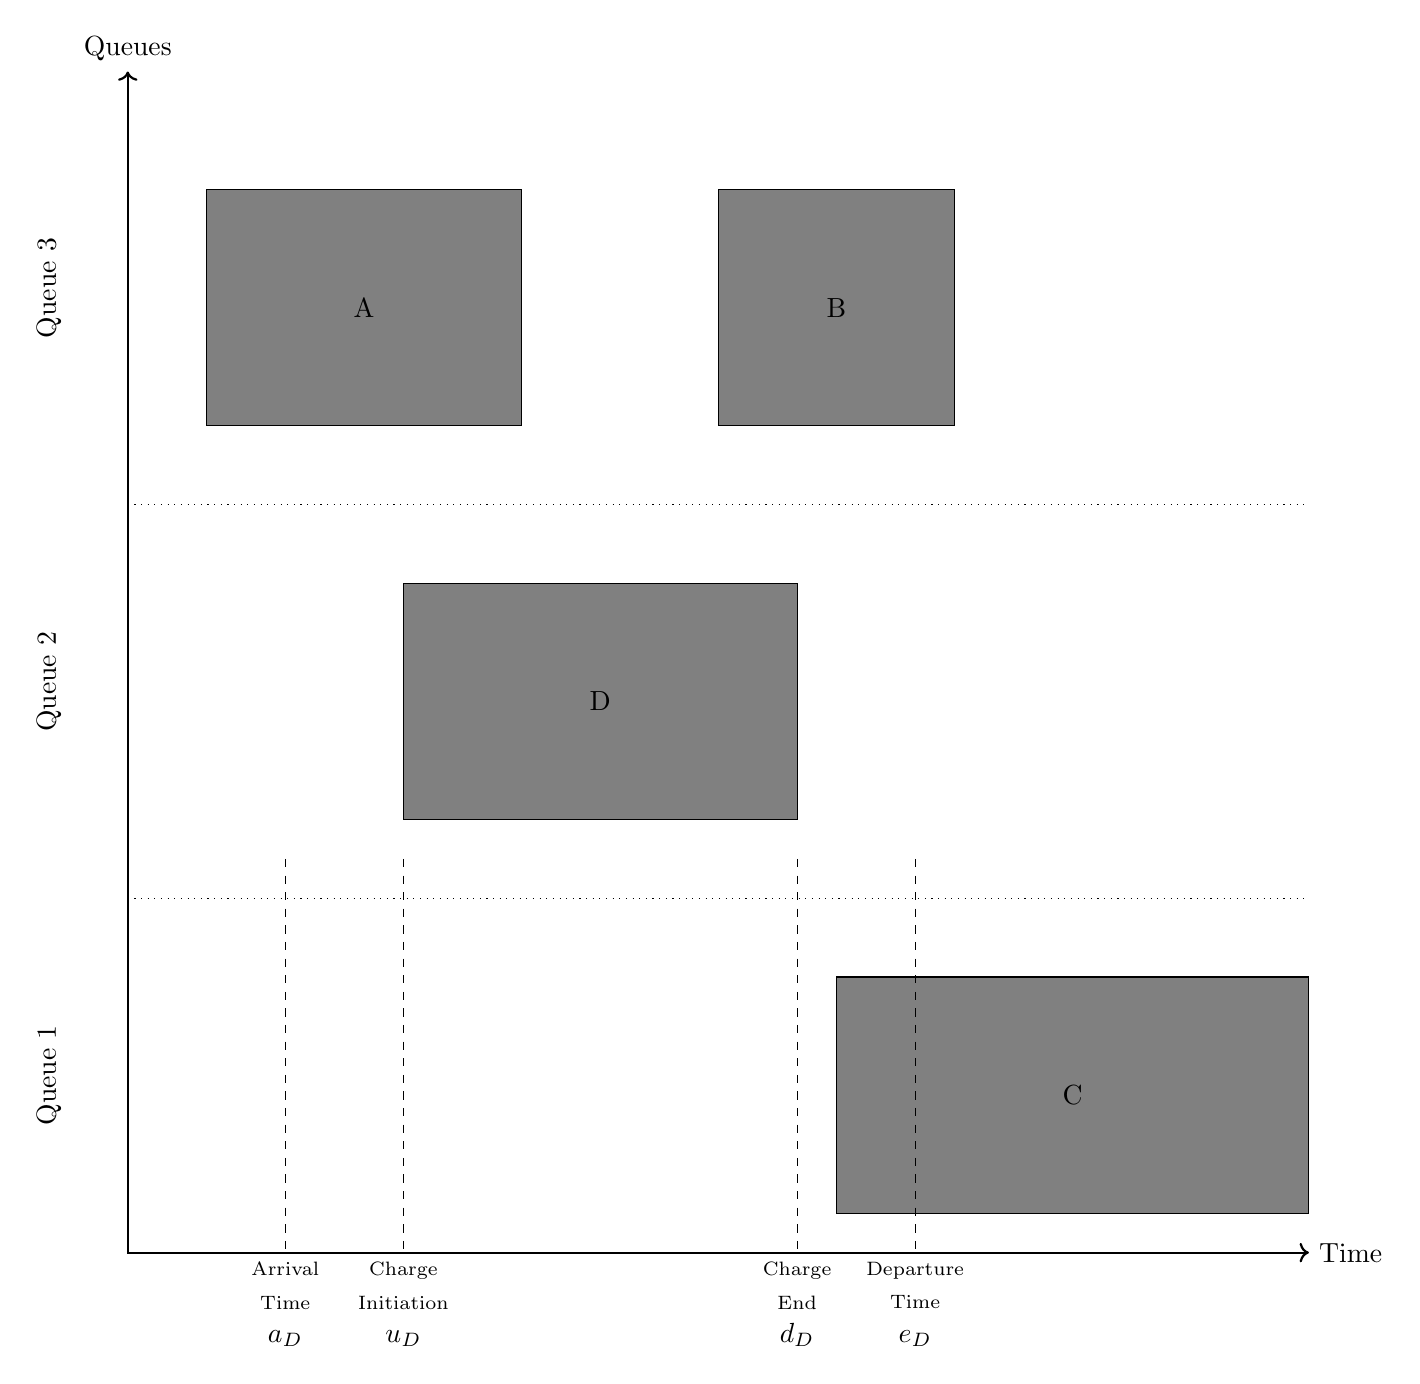
\begin{tikzpicture}
          % Variables
          \def \arrx   {2.0}
          \def \initx  {3.5}
          \def \endx   {8.5}
          \def \depx   {10.0}
          \def \yshift {5}

          % Axis
          \draw [thick,<->] (0,15) node[above]{Queues} -- (0,0) -- (15,0) node[right]{Time};

          % Rectangles
          \node[rectangle, draw, fill=gray, minimum width=4cm, minimum height = 3cm] at (3,12) {A};
          \node[rectangle, draw, fill=gray, minimum width=3cm, minimum height = 3cm] at (9,12) {B};
          \node[rectangle, draw, fill=gray, minimum width=5cm, minimum height = 3cm] at (6,7) {D};
          \node[rectangle, draw, fill=gray, minimum width=6cm, minimum height = 3cm] at (12,2) {C};

          % X-axis labels
          \node [below,align=center] at (\arrx,0) {\scriptsize Arrival     \\ \scriptsize Time \\ $a_D$};
          \node [below, align=center] at (\initx,0) {\scriptsize Charge    \\ \scriptsize Initiation  \\ $u_D$};
          \node [below, align=center] at (\endx,0) {\scriptsize Charge     \\ \scriptsize End \\ $d_D$};
          \node [below, align=center] at (\depx,0) {\scriptsize Departure  \\ \scriptsize Time \\ $e_D$};

          % Y-axis labels
          \node[rotate=90] at (-1, 2.25) {Queue 1};
          \node[rotate=90] at (-1, 7.25) {Queue 2};
          \node[rotate=90] at (-1, 12.25) {Queue 3};

          % Vertical lines
          \draw[dashed] (\arrx,\yshift)--(\arrx,0);
          \draw[dashed] (\initx,\yshift)--(\initx,0);
          \draw[dashed] (\endx,\yshift)--(\endx,0);
          \draw[dashed] (\depx,\yshift)--(\depx,0);

          % Horizontal lines
          \draw[dotted] (0, 4.5) -- (15, 4.5);
          \draw[dotted] (0, 9.5) -- (15, 9.5);

        \end{tikzpicture}
      }
      \caption{The representation of the queue-time space. The x and y-axis represent time and space, respectively. Along the y-axis, the dashed lines represent discrete queuing locations. The shaded rectangles represent schedules BEBs to be charged. The height of each shaded rectangle represents the space taken on the queue and the width being the time to service said BEB. The vertical dashed lines are associated with vessel D and represent the arrival time, initial charge time, charge completion time, and departure time. Note that the arrival time may be before the initial charge time and the completion time may before the departure time.}
      \label{fig:spacial-and-temporal-constr}
\end{figure}

\ref{seq:c0}-\ref{seq:c4} are denoted as ``queuing constraints''. They prevent overlap both spatially and temporally as
shown in \ref{fig:spacial-and-temporal-constr}. The y-axis represents the possible queues for a bus visit to be placed into, and the x-axis
represents the time that can be reserved for each visit. The shaded rectangles represent time that has been scheduled in
the horizontal direction, and the queue allocated for each bus visit in the vertical direction. In other words, the set
of constraints \ref{seq:c0} - \ref{seq:c4} aim to ensure that these shaded rectangles never overlap.

Constraint \ref{seq:c0} states that the starting charge time for BEB \(u_j\) must begin after the previous BEB departs,
\(d_i\). A value of \(\sigma_{ij} = 1 \implies\) bus \(i\) has detached from the charger before bus \(j\) has begun charging. If
\(\sigma_{ij} = 0\), then the constraint is of the form \(\T + d_i > u_j\) rendering the constraint ``inactive''. Similarly, for
\ref{seq:c1}, \(\psi_{ij}\) determines spacial positioning of BEB \(i\) and \(j\) relative to one another. A value of \(\psi_{ij} = 1
\implies\) BEB \(i\) is in a queue index that is less than BEB \(j\). If \(\psi_{ij} = 0\) then the constraint is deactivated.
Constraints \ref{seq:c2} - \ref{seq:c4} enforce spatial and temporal ordering between each queue/vehicle pair.
\ref{seq:c2} and \ref{seq:c3} ensure that BEB \(i\) is not placed before and after \(j\) spatially or temporally as that is
not possible. \ref{seq:c4} enforces at least one of the spatial or temporal relationships between each visit is active.
This ensures there are no scheduling conflicts (i.e. either charging sessions are ordered temporally or are in different
queues).

\ref{seq:c5} describes the service time of the bus. \ref{seq:c6} calculates the initial charge for the next visit for
bus \(b_i\). \ref{seq:c7} ensures that the bus is not being over-charged. \ref{seq:c8} ensures the continuity of the times
(i.e. the arrival time is less than the initial charge which is less than the detach time which is less than the time
the bus exits the station and all must be less than the time horizon).

\section{Simulated Annealing}
\label{sec:simulated-annealing}
SA is a well-studied local search metaheuristic used to solve various optimization problems
\cite{gendreau-2018-handb-metah,press-1992-numer-recip}. The algorithm is often applied to problems that contain many
local solutions as it employs a stochastic approach that explores the solution space for an approximate global optimum.
This model is named after its analogized process where a crystalline solid is heated then allowed to cool at a slow rate
until it achieves its most regular possible crystal lattice configuration (i.e. lowest energy state)
\cite{henderson-1989-theor-pract,press-1992-numer-recip}. SA establishes a connection between the thermodynamic
process and the search for global optimum in optimization problems. Within the SA process there are three key components:
cooling schedule, acceptance criteria, and generation mechanisms
\cite{keller-2019-multi-objec,press-1992-numer-recip}.

The cooling equation describes the speed at which the figurative temperature is decreased in a controlled manner over
time. Throughout the SA process, many ``candidate'' solutions are generated and compared to an ``active'' solution. The
method by which the solutions are accepted is determined by the acceptance criteria. The acceptance criteria is a
function of the system temperature that makes the decision whether the system will accept an inferior solution in favor
of exploring the solution space. The means by which candidate solutions are generated is via the generation mechanisms.
These generators modify the solution by some singular discrete change \cite{gendreau-2018-handb-metah}. Each of these
components are elaborated in the subsequent sections.

\subsection{Cooling Equation}
\label{cooling-equation-experimental}
The temperature function models a ``rate of cooling'' for the SA process. Initially, when the temperature is high, SA
encourages exploration. As the process begins to ``cools down'' (in accordance to the cooling schedule), it begins to
encourage local exploitation of the solution (rather than exploration)
\cite{rutenbar-1989-simul-anneal-algor,henderson-1989-theor-pract}. There are three common basic types of cooling
equations: linear, geometric, and exponential. Each schedule type is depicted in \ref{fig:cool}
\cite{keller-2019-multi-objec}. Every plot begins with an initial temperature of \(T_0 = 500^\circ\; C\) and a final
temperature of \(T_f = 1^\circ\; C\). The different cooling schedules dictate the rate at which the algorithm progressively
disallows exploration. Let the vector of temperatures described by a cooling schedule be defined as \(t\). Furthermore,
let an element of the vector be denoted as \(t_m \in t\), where \(m \in [0,...,M]\) and \(M = \lvert t \rvert\).

A linear cooling schedule is defined by \(t_m = t_{m-1} - \beta_0\). The terms utilized in \ref{fig:cool} are \(t_0 = \Tau_0\)
and \(\beta_0 = 1/2\; C^\circ\). An exponential cooling schedule is defined by the difference equation \(t_m = e^{-\beta_2}t_{m-1}\).
The values utilized in \ref{fig:cool} are \(\beta_2 = 0.01\). A geometric cooling schedules is as defined in \ref{eq:cool}. This
schedule type is most widely used in practice \cite{keller-2019-multi-objec}. As such, it will also be employed by this
work.

\begin{equation}
\label{eq:cool}
t_m = \beta t_{m-1}
\end{equation}

The gain variable, \(\beta\), in \ref{fig:cool} evaluated at \(\beta = 0.995\). The value of \(\beta\) may vary anywhere between the range
\([0,1)\). The further \(\beta\) is from 1, the quicker the function converges to zero. \ref{fig:geometric} demonstrates this
principle by plotting the geometric schedule using varying values of \(\beta\).

\begin{figure}[t!]
  \begin{subfigure}[t]{0.5\textwidth}
    \centering 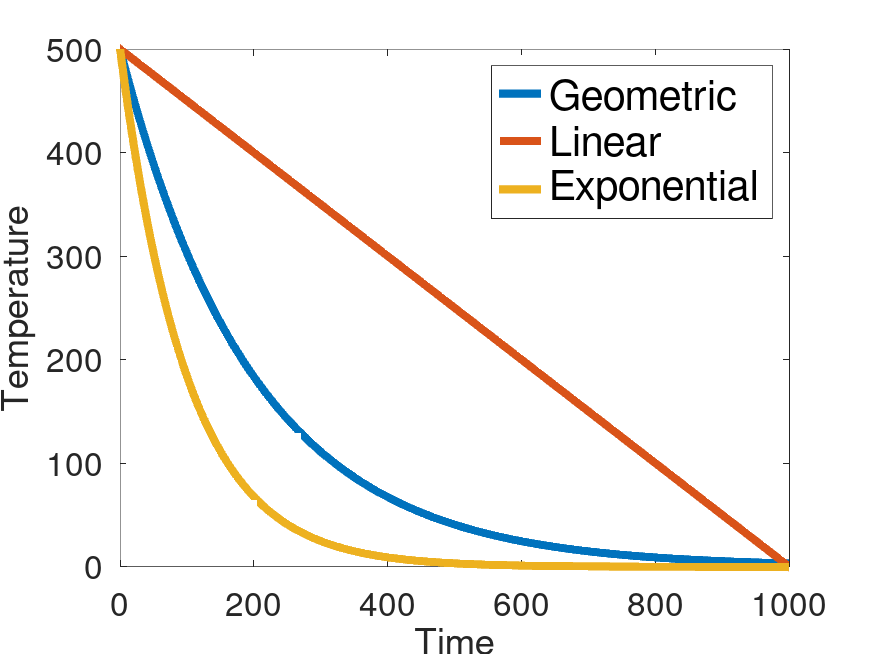
\includegraphics[width=\textwidth]{img/cool_func.png}
    \caption{Geometric, linear, and exponential cooling schedules.}
    \label{fig:cool}
  \end{subfigure}
  ~
  \begin{subfigure}[t]{0.5\textwidth}
    \centering 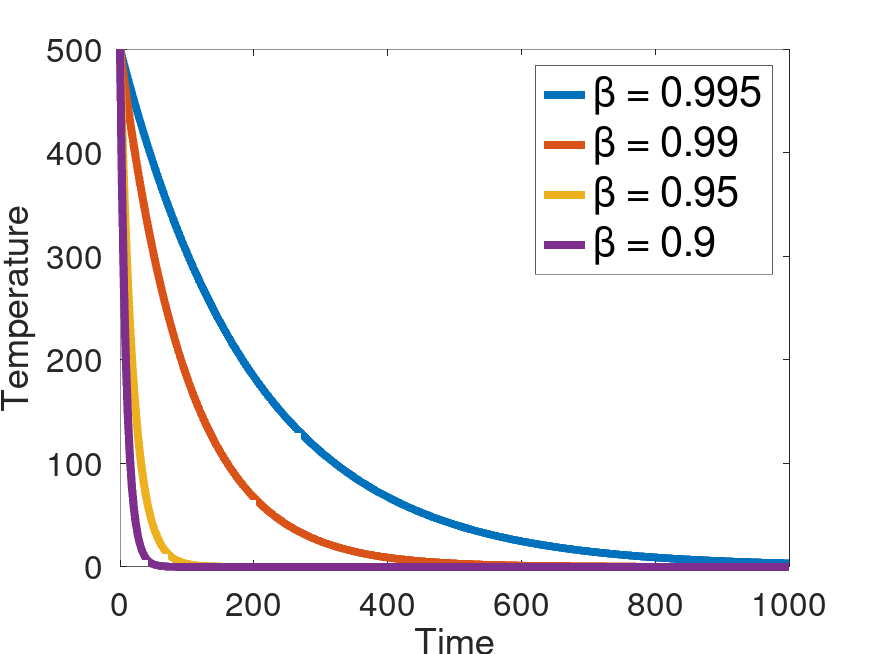
\includegraphics[width=\textwidth]{img/geometric.png}
    \caption{Geometric cooling schedule utilizing various value of $\beta$.}
    \label{fig:geometric}
  \end{subfigure}
\end{figure}

\subsection{Acceptance Criteria}
\label{sec:acceptance}
In SA, the algorithm stores a solution that is continuously compared to newly generated solutions. Let the stored
solution be referred to as the ``active solution''. During each iteration, a new ``candidate'' solution is generated and
compared to the active solution to determine if the candidate solution should replace the active solution. The method of
determining whether the active solution should be replaced is defined by an acceptance criteria. In an effort to
encourage exploration, inferior candidate solutions have a probability of being accepted. The probability of accepting
an inferior candidate solution is determined by the objective functions of the active and candidate solutions, \(J(\I)\)
and \(J(\bar{\I})\), respectively, and the current temperature, \(t_m\). Let \(\Delta E \equiv J(\I) - J(\bar{\I})\) and let \(f(\cdot)\) be
the function that describes the probability of accepting a candidate solution \(\bar{\I}\). The probability of accepting a
candidate solution is thus of the form \cite{keller-2019-multi-objec}

\begin{equation}
\label{eq:candaccept}
f(\I,\bar{\I},t_m) =
\begin{cases}
  1                   & \Delta E > 0 \\
  e^{- \frac{\Delta E}{t_m}} & \text{otherwise}
\end{cases}\text{.}
\end{equation}

\subsection{Neighbor Generators and Wrappers}
\label{sec:generation-mechanisms}
Generation mechanisms are used to create a neighboring candidate solution \cite{gendreau-2018-handb-metah}. That is,
the generating function creates a solution that can be reached in a single iteration from the active solution. In
response to the problem statement made in , five primitive generation mechanism are used: new
visit, slide visit, new charger, new window, wait. The purpose of each of these generators is to assign new visits to a
charger, adjust a bus visits initial and final charge time within the same time frame/queue, move a BEB from one charger
to another with the same charge schedule, move a bus to its idle queue. Each generator will be discussed in more detail
in \ref{sec:sa-generators}.

These generation mechanisms will in turn be utilized by two wrapper functions. The schedule generation is to used create
an initial candidate solutions for SA and the perturb schedule generator is used to take a candidate solution and alter
it slightly in an attempt to step toward a global or local minimum. The wrapper functions will be discussed in
\ref{sec:sa-generator-wrappers}. However, prior to discussing the primitives and wrapper generating functions, their respective
inputs and outputs must be defined.

\subsubsection{Generator Input/Output}
\label{sec:sa-generator-input-output}
Each generator accepts a tuple \(\Sol \equiv (i, \I, \C)\) where \(i\) is the visit index being manipulated, \(\I\) is the set of
visits, and \(\C\) is the set that describes the availability for all chargers \(q \in \Qset\). The output of the generating
functions is the same as the input, but with changes applied to it by a generator. Let a modified variable be denoted
with a bar, \(\bar{\cdot}\). Thus, the modified input tuple is written as \(\bar{\Sol}\).

\subsubsection{Generators}
\label{sec:sa-generators}
The mechanism by which candidate solutions are generated is to be introduced. Recall that to satisfy
constraints, \(n_B\) extra idle queues are added that provide no power to the BEB. Because of this, the set of queues is
fully defined where \(Q\) is the ordered set of idle queues, slow queues, then fast queue. The use case for the idle
queues are for when a bus is not to be placed on a charger. Rather, it will be placed in the queue, \(q \in B\), which
satisfies the previously defined spatial constraints while allowing the bus to be ``set aside''. The charge queues are
denoted by \(q \in \{1, ..., n_B , n_B + 1, ..., n_Q\}\).

Recall the dot notation is used to extract variables from tuples. For example, suppose the arrival time is desired to be
extracted from visit \(i\). Given \(\I\), the notation that describes extracting the initial charge time for visit \(i\) is
written as \(u_i \equiv \I_{i.u}\).

\paragraph{New visit}
\label{sec:sa-new-visit}
The new visit generator defined in \ref{alg:new-visit} describes the process of moving a BEB, \(b \in B\), from a waiting
queue, \(q \in B\), to a charging queue, \(q_i \in \{n_B + 1, ..., n_Q\}\), within its arrival/departure time \([a, e]\). Let
\(\U_{\{\cdot\}}\) indicate that an element is selected randomly with a uniform distribution from the set \(\{\cdot\}\). For
example, \(\U_{[a_i, e_i]}\) indicates that a value will be selected between \(a\) and \(e\) with a uniform distribution.
\ref{alg:new-visit} begins by extracting variables. Lines 6 and 7 randomly select a charging queue and available time
frame with a uniform distribution, respectively. Line 8 attempts to assign the visit the time frame found in Line 7, if
it succeeds, the updated visit is returned. Otherwise, the null value is returned.

The function \texttt{findFreeTime} is the algorithm that determines whether a visit's time at the station \([a_i, e_i]\) can be placed
in the time availability of charger \(q\). Let the available time for charger \(q\) for visit \(i\) be denoted as \(C \equiv
\C_{i.q}\). Furthermore, let the lower and upper bound of \(\C\) be denoted as \(C_L\) and \(C_U\), respectively. The algorithm
checks whether the BEB time at the station, \([a_i, e_i]\) fits within the charger availability \([C_L, C_U]\). If it does,
a random charging time frame is returned such that \(a_i \le u_i \le d_i \le e_i\). Otherwise the null value is returned.

\begin{algorithm}[H]
  \scriptsize
  \caption{New visit algorithm}
  \label{alg:new-visit}
  \LinesNumbered
  \TitleOfAlgo{New Visit}
  \KwIn{$\Sol$}
  \KwOut{$\bar{\Sol}$}

  \SetKwFunction{Union}{Union}
  \SetKwFunction{findFreeTime}{findFreeTime}

  \Begin
    {
      $i \leftarrow \Sol_{i}$\tcc*{Extract visit index}
      $a \leftarrow \I_{i.a}$\tcc*{Extract the arrivial time for visit $i$}
      $e \leftarrow \I_{i.e}$\tcc*{Extract the departure time for visit $i$}
      $q \leftarrow \I_{i.q}$\tcc*{Extract the current charge queue for visit $i$}
      $\bar{q} \leftarrow \mathcal{U}_{Q}$\tcc*{Select a random charging queue with a uniform distribution}
      $C \leftarrow \mathcal{U}_{\C_q}$\tcc*{Select a random time slice from $\C_q$}

      \If(\tcc*[f]{If there is time available in $C_q^j$}){($\bar{C}, \bar{u}, \bar{d}$) $\leftarrow$ \findFreeTime{$C, i, q, a, e$} $\not\in \varnothing$}
         {
           \Return{($i, (\bar{q},\bar{u},\bar{d}),\bar{C}$)}\tcc*[f]{Return visit}
         }

         \Return{($\varnothing$)}\tcc*{Return nothing}
    }
\end{algorithm}

\paragraph{Slide visit}
\label{slide-visit}
This primitive generator is used for visits that have already been scheduled. Because of the constraint \ref{seq:c8},
there may be some slack to manipulate \([u_i, d_i]\) within the window \([a_i, e_i]\). That is, two new values, \(u_i\) and
\(d_i\) are randomly selected with a uniform distribution that satisfy the constraint \(a_i \leq u_i \leq d_i \leq e_i\). Line 2 of
\ref{alg:slide-visit} purges the visit from the charger availability schedule. The \texttt{Purge} function simply removes an
assigned charge time from the set \(\C\). Without altering selected queue, the charge time randomly re-assigned with a
uniform distribution. Upon success, the updated tuple is returned, otherwise the null value is returned.

\begin{algorithm}[H]
  \scriptsize
  \caption{Slide Visit Algorithm} \label{alg:slide-visit}
  \LinesNumbered
  \TitleOfAlgo{Slide Visit}
  \KwIn{$\Sol$}
  \KwOut{$\bar{\Sol}$}

    \SetKwFunction{Purge}{Purge}

    \Begin
    {
      $(i, \I, \bar{\C}) \leftarrow$\Purge{$\Sol$}\tcc*{Purge visit $i$ from charger availibility matrix}
      $C \leftarrow \bar{C}_{i.q_i}$\tcc*{Get the time availability of the purged visit}

      \tcc{If there is time available in $C$}
      \If{($\bar{C}, \bar{u}, \bar{d}$) $\leftarrow$ \findFreeTime{$C$, $\Sol_i$, $\I_q$, $\I_{i.a}, \I_{i.e}$} $\not\in \varnothing$}
      {
        \Return{($i, \I, (\I_{i.q_i},\bar{u},\bar{d}),\bar{C}$)}\tcc*[f]{Return updated visit}
      }

        \Return{($\varnothing$)}\tcc*{Return nothing}
    }
  \end{algorithm}

\paragraph{New charger}
\label{new-charger}
The new charger generator moves a visit \(\I_i\) to a new charging queue while maintaining the same charge time, \([u_i,
d_i]\). \ref{alg:new-charger} purges the visit from the charger availability set, a queue is selected at random with a
uniform distribution, then the new selection is checked whether the charge time \([u_i, d_i]\) may be assigned to the new
queue.

\begin{algorithm}[H]
  \scriptsize
  \caption{New Charger Algorithm} \label{alg:new-charger} \LinesNumbered \TitleOfAlgo{New Charger} \KwIn{$\Sol$}
  \KwOut{$\bar{\Sol}$}

    \SetKwFunction{Purge}{Purge}

    \Begin
    {
      $(i, \I, \bar{\C}) \leftarrow$\Purge{$\Sol$}\tcc*{Purge visit $i$ from charger availibility matrix}
      $q \leftarrow \mathcal{U}_{Q}$\tcc*{Select a random charging queue with a uniform distribution}

      \If(\tcc*[f]{If there is time available in $C_{q}$}){($\bar{C}, \bar{u}, \bar{d}$) $\leftarrow$ \findFreeTime{$\bar{\C}_{i.q}$, $\Sol_i$, $\I_q$, $\I_{i.a}, \I_{i.e}$} $\not\in \varnothing$}
      {
        \tcc{Return visit, note $u$ and $d$ are the original inital/final charge times.}
        \Return{($i, \I, (q,\I_{i.u}, \I_{i.d}),\bar{\C}$)}
      }

      \Return{($\varnothing$)}\tcc*{Return nothing}
    }
  \end{algorithm}

\paragraph{Wait}
\label{sec:sa-wait}
The wait generator simply removes a bus from a charger queue and places it in its idle queue, \(q_i \in B\). \ref{alg:wait}
begins by purging the visit from the charger availability set, the visit is then assigned to its idle queue for the
duration of its time at the station.

\begin{algorithm}[H]
\scriptsize
\caption{Wait algorithm} \label{alg:wait}
    \LinesNumbered
    \TitleOfAlgo{Wait}
    \KwIn{$\Sol$}
    \KwOut{$\bar{\Sol}$}

    \SetKwFunction{Purge}{Purge}

    \Begin
    {
      $(i, \I, \bar{\C}) \leftarrow$\Purge{$\Sol$}\tcc*{Purge visit $i$ from charger availibility matrix}
      $\bar{\C}'_{\I_{i.\Gamma_i}} \leftarrow \C' \cup \{[\I_{i.a}, \I_{i.e}]\}$\tcc*{Update the charger availability matrix for wait queue $\bar{\C}_{i.q_i}$}
      \Return{$(i, \I, (\I_{i.b}, \I_{i.a}, \I_{i.e}), \bar{\C})$}\tcc*[f]{Return visit}
    }
  \end{algorithm}

\paragraph{New Window}
\label{sec:sa-new-window}
New window, as shown in \ref{alg:new-window}, is a combination of \ref{alg:new-visit} (new visit) and \ref{alg:wait}
(wait). By this it is meant that visit \(i\) is placed in its wait queue then added back in as if it were a new visit.
This implies that the BEB may be assigned to a different queue with a new charging time frame. Upon success, the
algorithm return the updated tuple, otherwise return the null value.

\begin{algorithm}[H]
  \scriptsize
  \caption{New window algorithm} \label{alg:new-window}
  \LinesNumbered
  \TitleOfAlgo{New Window}
  \KwIn{$\Sol$}
  \KwOut{$\bar{\Sol}$}

  \SetKwFunction{NewVisit}{NewVisit}
  \SetKwFunction{Wait}{Wait}

  \Begin
  {
    $\bar{\Sol} \leftarrow$\Wait{$\Sol$}\tcc*{Assign visit to its respective idle queue}
    \If(\tcc*[f]{Add visit $i$ back in randomly})
       {
         $\bar{\bar{\Sol}} \leftarrow$ \NewVisit{$\bar{\Sol}$} $\not\in \varnothing$
       }
       {
         \Return{$\bar{\bar{\Sol}}$} \tcc*[f]{Return visit}
       }

       \Return{($\varnothing$)}\tcc*{Return nothing}
  }
\end{algorithm}

\subsubsection{Generator Wrappers}
\label{sec:sa-generator-wrappers}
The generator wrappers provide the highest level of abstraction from which the SA algorithm will directly interact.
These wrapper functions utilize the primitive generators previously described to either create a new charge schedule to
initialize the SA algorithm, or to modify an existing schedule.

\paragraph{Charge Schedule Generation}
\label{sec:sa-charge-schedule-generation}
The objective of \ref{alg:charge-schedule-generation} is introduce a method that provides the SA algorithm with an
initial charging schedule. The schedule generation is chosen to initialize the algorithm in a greedier manner by looping
through each visit and executing \ref{alg:new-visit} to place visit \(i\) at random queue with a random charge time.

\begin{algorithm}[H]
\scriptsize
\caption{Charge schedule generation algorithm} \label{alg:charge-schedule-generation}
    \LinesNumbered
    \TitleOfAlgo{Candidate Solution Generator}
    \KwIn{$\Sol$}
    \KwOut{$\bar{\Sol}$}

    \SetKwFunction{NewVisit}{NewVisit}

    \Begin
    {
        \tcc{Select an unscheduled BEB visit from a randomly indexed set of visits}
        \ForEach {$\I_i \in \I$}
        {
            ($i, \bar{\I}$, $\bar{\C}$) $\leftarrow$ \NewVisit{($\I_i$, $\I$, $\C$)}\tcc*{Assign the bus to a charger}
        }
            \Return{($0, \bar{\I}$, $\bar{\C}$)}
    }
  \end{algorithm}

\paragraph{Perturb Schedule}
\label{sec:sa-tweak-schedule}
Once the active solution has been created by \ref{alg:charge-schedule-generation}, the SA process begins modifying it to
create candidate solutions. After each step of the cooling equation, the active solution will be altered \(n_K\) times by
a random primitive generator. During these \(n_K\) iterations the active solution is modified to create a neighboring
candidate solution. This candidate solution will then be compared against the active solution in the manner discussed in
. \ref{alg:perturb-schedule} describes the method by which the SA algorithm decides how to perturb the
schedule. The method that will be employed to generate neighboring solutions is as follows: pick a visit, pick a
primitive generator, and execute said primitive generator once. Let \(\W^y_{[\cdot]}\) denote a random selection with a
distribution specified by a weight vector \(y \in \mathbb{R}\). Thus, \ref{alg:perturb-schedule} is as follows: select a visit with a
uniform distribution, select a primitive with a weighted distribution. Letting \(n_G\) denote the number of primitive
generating functions, the selected primitive with a weighted distribution is denoted as \(\W^y_{[1, n_G]}\). The primitive
is then executed, and the results are returned.

\begin{algorithm}[H]
\scriptsize
\caption{Perturb schedule algorithm} \label{alg:perturb-schedule}

    \LinesNumbered
    \TitleOfAlgo{Perturb Schedule}
    \KwIn{$\Sol$}
    \KwOut{$\bar{\Sol}$}

    \SetKwFunction{PGF}{PGF}

    \Begin
    {
        $\I_i\leftarrow\; \U_{\I}$\tcc*{Randomly select a visit}
        $i \leftarrow\; \I_i$\tcc*{Extract visit index}
        $y \leftarrow [y_1, y_2, ...]$\tcc*{Define the weight of each primitive generator}
        $PGF \leftarrow\; \W^y_{[1,n_G]}$\tcc*{Select one of the generator functions}
        $\bar{\Sol} \leftarrow$ \PGF{($i$, $\I$, $\C$)}\tcc*{Excecute the generator function}
        \Return{($0, \bar{\I}$, $\bar{\C}$)}
    }
\end{algorithm}

\subsection{Alternative Heuristic Implementation}
\label{sec:heuristic-implementation}
As suggested by the works in \cite{Zhang_2010,Xinchao_2011}, applying heuristics to the generating functions can
manipulate the searched neighborhoods in a way that may assist the SA algorithm with convergence. As a test to assist in
minimizing charger utilization, a simple heuristic is applied to \ref{alg:new-visit} and \ref{alg:new-charger} in the
method that they select new charging queues. Rather than selecting a queue at random from \(q \in Q\), the algorithms
randomly select whether to place a BEB in a slow or fast charging queue with a weighted distribution favoring slow
chargers. Once the charger type has been selected, the algorithm will then begin incrementally attempting to place the
BEB in a queue of that type beginning from the smallest index of that charger type. For example, if a BEB has been
selected to be placed in a queue with a slow charger, the algorithm begins by attempting to place the BEB in the charger
queue \(q = n_B + 1\). If it is unable to be placed in that queue, it then attempts to be placed in the next queue \(q =
n_B + 2\). This is done incrementally until all the queues have been exhausted. The objective of this alternative
approach is to explore whether the added up-front computation cost by including the heuristic will positively influence
the output of the results and to what degree.

At the expense of an additional up-front
computation cost, the heuristic will attempt to pack the visit optimally in the spacial sense.

\section{Optimization Algorithm}
\label{sec:optimization-algorithm}
This section combines the generation algorithms and the optimization problem into a single algorithm (\ref{alg:sa-pap}).
Generally, SA assumes that the generated candidate solutions are within the solution space of the problem, \(\omega \in S\) where
\(S\) is the solution space. Hence, the initialization and perturbations of a schedule must be verified to ensure that the
generated schedule is in the solution space. Therefore, the objective function and constraints introduced in
\ref{sec:sa-constraints} and \ref{sec:sa-objective-function}, respectively, must be employed to verify that the outputs of
\ref{alg:charge-schedule-generation} and \ref{alg:perturb-schedule} are in the feasible space, \(S\).

As previously stated, the generating functions directly influence the values of the assigned charge queue, charge
initialization time, and charge completion time: \(q_i\), \(u_i\), and \(d_i\), respectively. Having generated those values,
the rest of the decision variables may be derived. Beginning with the packing constraints, \ref{seq:c0}-\ref{seq:c1} are
employed to enable and disable \(\sigma_{ij}\) and \(\psi_{ij}\) and \ref{seq:c2}-\ref{seq:c4} ensure the validity of the values.
\ref{seq:c5} can be directly calculated and \ref{seq:c8} is fully defined.

Changing the focus over to the dynamic constraints, similarly to what was seen with the packing constraints, the battery
dynamic constraints are also fully defined and can be calculated. \ref{seq:c6} is sequentially calculated after a given
schedule has been fully defined. \ref{seq:c7} is evaluated to ensure the BEB is not overcharged. The penalty method
implemented in \ref{sec:sa-objective-function} is set in place to allow the SOC to go below the specified threshold, \(\nu_{\Xi_i}
\kappa_{\Xi_i}\), but punish the solution for doing so. Thus, over time, the candidate solutions will be encouraged toward a
solution that does not activate the penalty method (i.e., is solution is operationally feasible).

The SA-PAP algorithm in \ref{alg:sa-pap} will now be outlined. The algorithm begins by creating a temperature schedule
and creating an initial solution. The algorithm then begins to iterate through the temperature schedule (outer loop).
For each iteration of the outer loop, an inner loop is executed \(n_K\) times. During this inner loop, the solution is
modified by a generating function to create a candidate solution. The candidate is solution is then compared with the
active solution, and updated according to the acceptance criteria. These actions are performed until the cooling
equation is exhausted.

\begin{algorithm}[H]
  \scriptsize
  \caption{Simulated annealing approach to the position allocation problem} \label{alg:sa-pap}
  \LinesNumbered
  \TitleOfAlgo{SA PAP}
  \KwIn{($\I$ , $\C$)}
  \KwOut{($\bar{\I}$, $\bar{\C}$)}

  \SetKwFunction{Temp}{$\Tau$}
  \SetKwFunction{CSG}{CSG}
  \SetKwFunction{PS}{PS}
  \SetKwFunction{Obj}{J}

  \Begin
    {
      \tcc{Generate vector of temperatures given cooling equation $\Tau$ and initial temperature $\Tau_0$}
      $t \leftarrow$ \Temp{$\Tau_0$}

      $\Sol \leftarrow$\CSG{($\I$, $\C$)}\tcc{Generate an initial solution}

      \tcc{For each item in the temperature vector}
      \ForEach{$t_k \in t$}
       {
        \tcc{For each step in the constant temperature repitition counter}
        \ForEach{$k \in \{0, 1, ..., n_K\}$}
        {
          $\bar{\Sol} \leftarrow$ \PS{($\I$, $\C$)} \tcc*{Generate a new solution}
          $\Delta E = $ \Obj{$\bar{\Sol}_{\I}$}  - \Obj{$\Sol_{\I}$} \tcc*{Calculate the difference of fitness scores}

          \If{$\bar{\I} \in S$ and $\Delta E < 0$}{$\Sol \leftarrow \bar{\Sol}$}
          \If{$\bar{\I} \in S$ and $\Delta E \ge 0$}{$\Sol \leftarrow \bar{\Sol}$ with probability $e^{\frac{\Delta E}{t_k}}$}
        } % For k
      }   % For t_k \in t

      \Return{($\I$ , $\bar{\C}$)}
    } % Begin
\end{algorithm}

\section{Example}
\label{sec:sa-pap-example}
An example is now provided to demonstrate the utility of the developed SA charge scheduling technique. In
\ref{sec:sa-beb-scenario} a description of the example scenario is presented followed by a brief introduction of the original
MILP PAP. An alternative threshold based planning strategy called the Qin-Modified technique, and a heuristic
modification to the SA PAP are also used as comparisons to the SA PAP technique presented in this work. \ref{sec:sa-results}
presents the results for each of planning strategies. The results are then analyzed and discussed.

\subsection{BEB Scenario}
\label{sec:sa-beb-scenario}
The test scenario was run over a time horizon of \(T=24\) hours, with a total of \(n_V = \N\) visits to the station shared
between \(n_B = \A\) buses. Each BEB is assumed to have a battery capacity of \(\kappa_b =\) \batsize kWh that is required to
stay above an SOC of \(\nu_b =\) \mincharge (\fpeval{\batsize * \minchargeD} kWh). Each bus is assumed to begin
the working day with \(\alpha =\) \fpeval{\acharge*100}\% charge (\fpeval{\acharge * \batsize} kWh). A
total of \(n_C =\) \fpeval{\fast + \slow} chargers are utilized where \slow of the chargers are slow charging
(\slows kW) and \fast are fast charging (\fasts kW). The gains of \(z_p = \Cgain\), \(z_c = 1\), and \(z_d
= 10000\) are used. As previously introduced, to encourage the SA PAP to utilize the fewest number of
chargers, the value of \(\epsilon_q\) in the objective function is \(\forall q \in \{1,2,..., n_B \}; \epsilon_q = 0\) and \(\forall q \in \{n_B + 1, n_B +
2, ..., n_Q\}; \epsilon_q = 100q\). The SA algorithm utilizes the geometric cooling schedule with an initial temperature of \(T_0
= \tempinit\) with \(\beta_2 = 0.999\), resulting in a total of \(n_M = \tempcnt\) steps. Rocky Mountain Power utilizes fifteen
minute intervals to calculate the demand cost \cite{rocky-mountain-power}. Thus, the demand cost is calculated
utilizing \(T_p =\) \fpeval{15*60} second intervals. A weight vector of \([3, 3, 2, 1]\) is used to influence
the distribution of selecting the new charger, new window, wait, and slide visit primitives, respectively. The algorithm
also assumes a total of \(n_K = \localcnt\) iterations for the local search at a constant temperature. In total, that
results in \fpeval{\localcnt * \tempcnt} configurations being searched. On average each constant temperature
search took an average of \(\quicklocal\) seconds to complete, resulting in a total runtime of
\fpeval{\quicklocal * \tempcnt} seconds.

introduced the idea of an alternative heuristic implementation for the SA algorithm. To
distinguish the heuristic implementation from the method derived in , let this
implementation be referred to as ``heuristic'' implementation and the previous as the ``quick'' implementation due to the
fact that it is designed to execute more quickly. Using the same weights for randomly selecting the primitive
generators, the heuristic approach further implemented a weighted distribution vector of \([3, 1]\) to decide whether to
select a slow or fast charger, respectively. In the heuristic approach, on average the constant temperature search took
a total of \(\heuristiclocal\) seconds to complete, resulting in a total runtime of \fpeval{\heuristiclocal * \tempcnt} seconds. The heuristic generators were expected to be slightly slower due to its iterative approach.

The Qin-Modified is a threshold-based strategy that is also employed as a means of comparison with the results of the SA
PAP. The Qin-Modified algorithm is a based on the threshold strategy of \cite{qin-2016-numer-analy}. The algorithm has
been modified slightly to accommodate the case of multiple charger types without a heuristic search for the best charger
type. The heuristic is based on a set of rules that revolve around the initial charge of the bus at visit \(i\). There are
three different thresholds, low (85\%), medium (90\%), and high (95\%). Buses below the low threshold are prioritized to
fast chargers then are allowed to utilize slow chargers if no fast chargers are available. Buses between the low and
medium threshold prioritize slow chargers first and utilize fast chargers only if no slow chargers are available. Buses
above the medium threshold and below high will only be assigned to slow chargers. Buses above the high threshold will
not be charged. Once a bus has been assigned to a charger, it remains on the charger for the duration of the time it is
at the station, or it reaches 95\% charge, whichever comes first. Note that UTA sets their high threshold at 70\% with the
other respective thresholds being lowered as well. The higher thresholds implemented in this work were selected in
attempt to improve the results of the Qin-Modified technique given the specified scenario.

Another methods utilized to compare with against SA PAP is what is known as the MILP PAP. This framework is the original
MILP implementation of the PAP derived from \cite{qarebagh-2019-optim-sched}. Because this method employs a solver that
can guarantee optimality, the MILP implementation is utilized in this work as a benchmark for the other schedules. The
inputs to the system are the same as those discussed above. It is of note that the MILP PAP does not implement the
demand cost in its objective function. In an attempt to compare the solution of the MILP with the SA output more
directly, a similar solve time of 3600 seconds is utilized. The MILP was executed using the Gurobi MILP solver
\cite{gurobi-2021-gurob-optim}. The previously described simulations were run on a machine equipped with an AMD Ryzen 9
5900X 12 - Processor (24 core) at 4.95GHz.

\subsection{Results}
\label{sec:sa-results}
The schedules generated by each of the methods is presented in \ref{fig:schedule}. Rows 0-14 represent slow charging
queues and rows 15-29 represent fast charging queues. The symbols represent the initial charge times, and the horizontal
line with the vertical tick signifies the region of time the charger is active. A qualitative comparison between the
different schedules is the sparsity of the quick SA technique. Although the assignment cost was set in place, due to the
random nature of the queue assignments the simulation was not able to converge to a well-packed or ``dense'' solution. The
heuristic approach was able to more successfully able to pack its schedule similarly to the schedule of the MILP PAP.
The Qin-Modified strategy was able to create a very dense schedule that is simple to employ.

On the quantitative side of the minimization/packing discussion, the Qin-Modified schedule utilizes one fast and two
slow chargers as can be seen in \ref{subfig:schedule-qin}. The MILP PAP framework generated a schedule that utilizes
three fast charges and four slow chargers as shown in \ref{subfig:schedule-milp}. The heuristic SA strategy created a
schedule with eight slow charger queues and four fast charging queues as shown in \ref{subfig:schedule-heuristic-sa}.
The quick strategy for the SA algorithm created a schedule utilizing fifteen slow and fast chargers as is demonstrated
in \ref{subfig:schedule-quick-sa}. That is to say, the Qin-Modified schedule was able to most effectively minimize the
charger count followed by the MILP PAP, and the heuristic SA, the worst being the quick SA technique. The MILP produced
a schedule with a three charger gap in the fast queues, where the intermediate queues were never used. The heuristic SA,
while possibly being able to move some assignments to a lower charge queue index (i.e., create a ``denser'' schedule), did
not contain any gaps of unused queues. The Qin-Modified utilized the fewest chargers overall. It is worth noting here
that the SA algorithm has no guarantee of optimality; therefore, post-processing could be applied to further minimize
the charger indices in an attempt to create a more dense schedule.

The row labeled ``max'' in \ref{tab:charge-count} tabulates the total amount of queues the system actually utilized in
parallel while the schedule row represents the amount of queues the particular schedule requests. Referencing the slow
charger columns in \ref{tab:charge-count}, the Qin-Modified only utilized 2 slow chargers and only requests two slow
charging queues. Looking at \ref{subfig:schedule-qin} it is observed that the slow charging queues cannot be further
reduced. Similarly, the MILP used a maximum of 4 chargers in parallel which is the same as the required amount of queues
by the schedule. By referencing \ref{subfig:schedule-milp}, it can be seen that the slow chargers cannot be minimized
any further. The quick SA technique utilized every slow charger, but only employed a maximum of six chargers in
parallel. This gives a measure to how the queues were sparsely placed as with appropriate packing, only six queues are
theoretically required with the provided schedule. The heuristic SA utilized a maximum of seven chargers although the
total queues required by the schedule is nine. As stated before, post-processing could be applied to alleviate this
problem, although the schedule would still not being quite as well packed as the Qin-Modified or MILP schedules.

Similarly for the fast chargers, the Qin-Modified only utilized a single charging queue. The MILP calls for a total of
three queues, but only ever has a maximum use of two with being utilized at any given moment. The quick SA again
utilized every fast charger available with a maximum of two chargers being utilized in parallel. The heuristic SA
technique required four fast charging queues but only used two in parallel. Thus, the Qin-Modified scheduled was able to
pack the schedule the most efficiently followed by the MILP and heuristic SA schedules.

\begin{table}[htbp]
\caption{\label{tab:charge-count}Table of the maximum amount of chargers used in parallel throughout the time horizon. The schedule row indicates the number of queues required by each schedule.}
\centering
\begin{tabular}{l|ll|ll|ll|ll}
\hline
 & MILP &  & Qin-Modified &  & Heuristic &  & Quick & \\[0pt]
\hline
 & Slow & Fast & Slow & Fast & Slow & Fast & Slow & Fast\\[0pt]
Max & 4 & 2 & 2 & 1 & 7 & 2 & 6 & 2\\[0pt]
Schedule & 4 & 3 & 2 & 1 & 9 & 4 & 15 & 15\\[0pt]
\hline
\end{tabular}
\end{table}

\ref{fig:charge} depicts the initial SOC for each visit throughout the simulation of each framework. \ref{tab:charge}
tabulates the mean, minimum, and maximum SOC upon arrival for each visit. The MILP PAP requires each BEB to stay above
an SOC of 25\% while the quick and heuristic SA approaches heavily penalize a schedule for allowing a BEB to go below the
25\% SOC threshold. The MILP PAP was able to successfully keep the SOC above the threshold (\ref{subfig:milp-charge})
while both SA approaches were not. The SOC of the quick SA approach dropped to a minimum of 29.9 kWh and the heuristic
had a minimum SOC of 6.3 kWh as shown in \ref{tab:charge}. The Qin model allowed the SOC of two BEBs to reach an SOC of
0\% as shown in \ref{subfig:qin-charge}. The Qin-Modified strategy, being a purely reactive model, is unable to ``sense''
whether a set of routes has a particularly taxing route later in the time horizon. As such, and in the case of the
example scenario, the BEBs that reached charges of 0\% began with a sequence of short routes, much like the other BEBs.
However, rather than continuing this trend, these sets of routes had one or two longer routes which the Qin-Modified
algorithm was unable to account for. To remedy this problem, a safety factor could be introduced to artificially
increase the threshold, \(S_f \nu_{\Xi_i}\kappa_{\Xi_i}\) where \(S_f > 1;\; S_f \in \mathbb{R}\). Interestingly, Qin-Modified strategy was able
to keep the mean SOC the highest followed by the quick SA, heuristic SA, and then the MILP. This is most likely due to
the higher placement of the low, medium, and high thresholds applied to the algorithm than what is used by Rocky
Mountain Power. This measure is useful when viewing with respect to \ref{fig:power} and \ref{fig:energy-usage}.

\begin{table}[htbp]
\caption{\label{tab:charge}Table of mean, min, and max SOC (kWh) for each charging schedule.}
\centering
\begin{tabular}{l|cccc}
\hline
 & MILP & Qin-Modifid & Heuristic & Quick\\[0pt]
\hline
Mean & 179.580229533742 & 292.615759538128 & 189.525113828846 & 216.523166855178\\[0pt]
Min & 96.9999999999463 & 0 & 6.3432083 & 29.862568\\[0pt]
Max & 388 & 368.6 & 388 & 388\\[0pt]
\hline
\end{tabular}
\end{table}

\ref{fig:power} depicts the power consumption over the time horizon for each model. As previous stated, the Qin-Modified
schedule had the highest mean SOC over the working day. Referencing \ref{fig:power-usage-milp-qin}, the Qin, while
staying below 1000 kW, is held at that level of power consumption for long periods of time. Similarly, the quick SA,
heuristic SA, and the MILP show that as the average SOC goes down, so does the demand. That is, there is a correlation
that suggests that if a schedule has a lower average SOC, the required demand (and total energy consumption which will
be discussed shortly) is also lower.

\ref{fig:power} is also of interest as it plots the peak power demand over the time horizon. The peaks in descending
order are: the quick and heuristic SA, tied at 1191.9 kW, the MILP at 1910 kW, and then the Qin at 970 kW. Although the
Qin had the lowest peak, it is again worth noting that the Qin-Modified technique was unable to keep the SOC of all the
BEBs above 0\%. The MILP and quick and heuristic SA are comparable in terms of the demand cost having a total difference
of \fpeval{1191.9 - 1910} kW. However, when viewing the mean power consumption in descending order paints a
different picture. The largest mean power demand is the Qin-Modified at 424.95 kW, quick SA at 257.98 kW, heuristic SA
at 198.84 kW, and then the MILP at 177.34 kW. The Qin-Modified, as shown in \ref{fig:power-usage-milp-qin}, although
having the lowest peak, holds the power for a long duration as previously discussed. This directly correlates into the
energy consumed by each schedule.

\begin{table}[htbp]
\caption{\label{tab:power}Table of mean and max power demand for each charging schedule.}
\centering
\begin{tabular}{l|cccc}
\hline
 & MILP & Qin-Modified & Heuristic & Quick\\[0pt]
\hline
Mean & 177.34 & 424.95 & 198.84105 & 257.9823\\[0pt]
Max & 1910 & 970 & 1911.9 & 1911.9\\[0pt]
\hline
\end{tabular}
\end{table}

The total energy consumed by each schedule is shown in \ref{fig:energy-usage}. The ordering of most energy consumed to
least is as follows: Qin-Modified, quick SA, heuristic SA, and the MILP PAP. The respective energy consumption for each
technique is: 10198.799 kWh, 6303.1704 kWh, 4797.746 kWh, and 4256.746 kWh. The heuristic SA consuming about 988 kWh
more than the MILP PAP.

\begin{figure}
  \centering
  %%~~~~~~~~~~~~~~~~~~~~~~~~~~~~~~~~~~~~~~~~~~~~~~~~~~~~~~~~~~~~~~~~~~~~~~~~~~~~
  % Qin
  \begin{subfigure}[t]{\textwidth}
    \centering
    \includegraphics[width=\textwidth]{sup-doc/sa-pap-paper/img/schedule-quinn}
    \caption{Charging schedule generated by Qin Modified algorithm.}
    \label{subfig:schedule-qin}
  \end{subfigure}

  \hfill

  %%~~~~~~~~~~~~~~~~~~~~~~~~~~~~~~~~~~~~~~~~~~~~~~~~~~~~~~~~~~~~~~~~~~~~~~~~~~~~
  % MILP
  \begin{subfigure}[t]{\textwidth}
    \centering
    \includegraphics[width=\textwidth]{sup-doc/sa-pap-paper/img/schedule-milp}
    \caption{Charging schedule generating by the MILP PAP algorithm.}
    \label{subfig:schedule-milp}
  \end{subfigure}
\end{figure}

\begin{figure} \ContinuedFloat
  \centering

  %%~~~~~~~~~~~~~~~~~~~~~~~~~~~~~~~~~~~~~~~~~~~~~~~~~~~~~~~~~~~~~~~~~~~~~~~~~~~~
  % SA heuristic
  \begin{subfigure}[t]{\textwidth}
    \centering \includegraphics[width=\textwidth]{sup-doc/sa-pap-paper/img/schedule-sa-heuristic}
    \caption{Charging schedule generated by the SA PAP algorithm using the heuristic strategy.}
    \label{subfig:schedule-heuristic-sa}
  \end{subfigure}

  \hfill

  %%~~~~~~~~~~~~~~~~~~~~~~~~~~~~~~~~~~~~~~~~~~~~~~~~~~~~~~~~~~~~~~~~~~~~~~~~~~~~
  % SA quick
  \begin{subfigure}[t]{\textwidth}
    \centering \includegraphics[width=\textwidth]{sup-doc/sa-pap-paper/img/schedule-sa-quick}
    \caption{Charging schedule generated by SA PAP algorithm using the quick strategy.}
    \label{subfig:schedule-quick-sa}
  \end{subfigure}
  \caption{Vairous schedules generated by the different frameworks. The horizonontal line stemming from the nodes ending with a vertical tick indicate the charge duration for that particular visit.}
  \label{fig:schedule}
\end{figure}

\begin{figure}
    %%~~~~~~~~~~~~~~~~~~~~~~~~~~~~~~~~~~~~~~~~~~~~~~~~~~~~~~~~~~~~~~~~~~~~~~~~~~~~
    % Fast
    \begin{subfigure}[t]{\textwidth}
    \centering
        \includegraphics[width=\textwidth]{sup-doc/sa-pap-paper/img/charger-count-fast-milp-qin}
        \caption{Number of fast chargers for Qin and MILP PAP.}
        \label{subfig:fast-charger-usage-milp-qinn}
    \end{subfigure}

    \begin{subfigure}[t]{\textwidth}
    \centering
        \includegraphics[width=\textwidth]{sup-doc/sa-pap-paper/img/charger-count-fast-sa}
        \caption{Number of fast chargers for quick and heuristic SA executions.}
        \label{subfig:fast-charger-usage-sa}
    \end{subfigure}
\end{figure}

\begin{figure}
    %%~~~~~~~~~~~~~~~~~~~~~~~~~~~~~~~~~~~~~~~~~~~~~~~~~~~~~~~~~~~~~~~~~~~~~~~~~~~~
    % Slow
    \begin{subfigure}[t]{\textwidth}
    \centering
        \includegraphics[width=\textwidth]{sup-doc/sa-pap-paper/img/charger-count-slow-milp-qin}
        \caption{Number of slow chargers for Qin and MILP PAP.}
        \label{subfig:slow-charger-usage-milp-qinn}
    \end{subfigure}
    \begin{subfigure}[t]{\textwidth}
    \centering
        \includegraphics[width=\textwidth]{sup-doc/sa-pap-paper/img/charger-count-slow-sa}
        \caption{Number of slow chargers for the quick and heuristic SA executions.}
        \label{subfig:slow-charger-usage-sa}
    \end{subfigure}
\end{figure}

\begin{figure}
  %%~~~~~~~~~~~~~~~~~~~~~~~~~~~~~~~~~~~~~~~~~~~~~~~~~~~~~~~~~~~~~~~~~~~~~~~~~~~~
  % Qin
  \begin{subfigure}[t]{\textwidth}
    \centering
    \includegraphics[width=\textwidth]{sup-doc/sa-pap-paper/img/charge-quinn}
    \caption{Bus charges for the Qin Modified charging schedule.}
    \label{subfig:qin-charge}
  \end{subfigure}
  \hfill
  %%~~~~~~~~~~~~~~~~~~~~~~~~~~~~~~~~~~~~~~~~~~~~~~~~~~~~~~~~~~~~~~~~~~~~~~~~~~~~
  % MILP
  \begin{subfigure}[t]{\textwidth}
    \centering
    \includegraphics[width=\textwidth]{sup-doc/sa-pap-paper/img/charge-milp}
    \caption{The bus charges for the MILP PAP charging schedule.}
    \label{subfig:milp-charge}
  \end{subfigure}
  \hfill
\end{figure}

\begin{figure}\ContinuedFloat
  %%~~~~~~~~~~~~~~~~~~~~~~~~~~~~~~~~~~~~~~~~~~~~~~~~~~~~~~~~~~~~~~~~~~~~~~~~~~~~
  % SA Quick
  \begin{subfigure}[t]{\textwidth}
    \centering
    \includegraphics[width=\textwidth]{sup-doc/sa-pap-paper/img/charge-sa-quick}
    \caption{The bus charges for the quick SA PAP charging schedule.}
    \label{subfig:sa-quick-charge}
  \end{subfigure}
  \hfill
  %%~~~~~~~~~~~~~~~~~~~~~~~~~~~~~~~~~~~~~~~~~~~~~~~~~~~~~~~~~~~~~~~~~~~~~~~~~~~~
  % SA Heuristic
  \begin{subfigure}[t]{\textwidth}
    \centering
    \includegraphics[width=\textwidth]{sup-doc/sa-pap-paper/img/charge-sa-heuristic}
    \caption{The bus charges for the heuristic SA PAP charging schedule.}
    \label{subfig:sa-heuristic-charge}
  \end{subfigure}
  \caption{Plots of the initial SOC of each visit over the time horizon for each schedule.}
  \label{fig:charge}
\end{figure}

\begin{figure}
  \begin{subfigure}[t]{\textwidth}
    \centering
    \includegraphics[width=\textwidth]{sup-doc/sa-pap-paper/img/power-milp-qin}
    \caption{Amount of power consumed by Qin-Modified and MILP schedules over the time horizon.}
    \label{fig:power-usage-milp-qin}
  \end{subfigure}

  \hfill

  \begin{subfigure}[t]{\textwidth}
    \centering
    \includegraphics[width=\textwidth]{sup-doc/sa-pap-paper/img/power-sa}
    \caption{Amount of power consumed by quick and heuristic SA schedules over the time horizon.}
    \label{fig:power-usage-sa}
  \end{subfigure}
  \caption{Amount of power consumed by each of the schedules over the time horizon.}
  \label{fig:power}
\end{figure}

\begin{figure}[htpb]
\centering \includegraphics[width=\textwidth]{sup-doc/sa-pap-paper/img/energy}
    \caption{Total accumulated energy consumed by the Qin-Modified, MILP, quick and heuristic SA schedules throughout the time horizon.}
    \label{fig:energy-usage}
\end{figure}

\chapter{A SIMULATED ANNEALING APPROACH WITH NON-LINEAR BATTERY DYNAMICS}
\label{sec:nonlinear-battery-dynamics}
The models presented up to this point have employed linear battery dynamic models to estimate the SOC of the BEB during
its charging phase. While linear battery dynamics are accurate up to about an 80\% SOC \cite{liu-2020-batter-elect},
fidelity is lost after this point due to the non-linearity of the charge profile. This chapter introduces a method of
replacing the linear battery dynamics throughout this work with a non-linear dynamics model. The non-linear model will
be employed in the SA algorithm from \ref{sec:sa-pap}. The chapter proceeds as follows: an introduction to the non-linear
battery dynamics model is shown in \ref{sec:nonlinear-model} along with a proof and description of how the model is
incorporated. \ref{sec:nonlinear-results} presents and discusses the results.

\section{Non-linear Battery Dynamics Model}
\label{sec:nonlinear-model}
Modeling the charging dynamics is imperative to the model's accuracy as it is one of the main factors in terms of the
decision variables. If the SOC is improperly modeled, that will produce an erroneous depiction of the state of BEB
charges and could result in over or under charging. Thus, care must be taken into considering the BEB's charging model.
There are various methods of modeling the SOC of a battery and can vary in complexity based on the attempt to
incorporate temperature, battery degradation, and current
\cite{zhang-2021-optim-elect,chen-2008-desig-grey,watrin-2012-multip-lithium}.

Some of the conventional methods to charge batteries are: Constant Voltage (CV), Constant Current (CC), and Constant
Current Constant Voltage (CCCV) \cite{arabsalmanabadi-2018-charg-techn}. In CCCV, a constant current is applied to a
battery until it reaches terminal voltage. Once this point has been reached, a constant voltage is applied as the charge
current decreases and the battery reaches full charge \cite{chen-2008-desig-grey}. Thus, by extension, CV merely
applies a constant voltage and CC a constant current \cite{arabsalmanabadi-2018-charg-techn}.

As previously stated, the SOC can be accurately modeled until the battery reaches a charge of about 80\%
\cite{liu-2020-batter-elect}. At this point the SOC becomes non-linear. Naturally, it has been suggested by
\cite{zhang-2021-optim-elect} that the SOC can be broken down into a linear and non-linear component. A plot of the SOC
for a battery is shown in to demonstrate these components \cite{zhang-2021-optim-elect}.

\begin{figure}

  \begin{minipage}{0.5\textwidth}
    \centering
    \includegraphics[width=0.9\textwidth]{img/soc-plot.png}
    \captionof{figure}{Illustration of non-linear charging profile.}
    \label{fig:soc-plot}
  \end{minipage}%
  \begin{minipage}{0.5\textwidth}
    \centering
    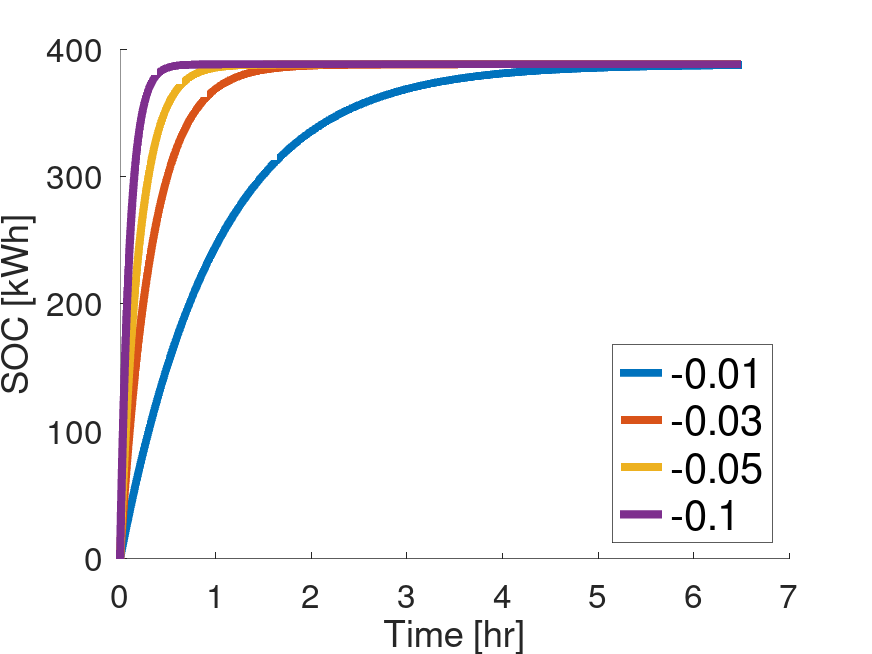
\includegraphics[width=0.9\textwidth]{img/nonlinear-bat.png}
    \captionof{figure}{Charging profiles for various convergence rates.}
    \label{fig:convergence-rates}
  \end{minipage}

\end{figure}

While some leverage the linear and non-linear components to derive their SOC model \cite{abdollahi-2016-optim-batter},
others have derived a first order equation to model this behavior \cite{whitaker-2023-a-network}. Assume that a charge
will occur over \(dt\) seconds. The SOC on the time step \(h+1\) for bus \(i\) can be determined by the simple discrete first
order equation

\begin{equation}
  \eta_{\xi_i} = \bar{a}_q \eta_i - \bar{b}_q \kappa_{\Xi_i}\text{,}
\end{equation}

where

\begin{equation}
\begin{array}{cc}
  \bar{a}_q = e^{a_q dt} & \bar{b}_q = e^{a_q dt} - 1\text{.}
\end{array}
\end{equation}

The equation is developed by using exact discretization \cite{brogan-1990-moder-contr-theor}, and is proved in
\cite{whitaker-2023-a-network}. The lemma and proof are subsequently shown for completeness.

\begin{lemma}
Assume that the charge will occur over intervals over $\Delta$ seconds, the charge at time step $k+1$ for visit $i$ can be related to the charge at time step $k$ using charger $q$ as

\begin{equation}
\eta_{i,k+1} = \bar{a}_{q_i} \eta_{i,k} - \bar{b}_{q_i} M_i\text{,}
\end{equation}

where $\eta_{i, k}$ represents the SOC for bus $i$ at step $k$ and

\begin{equation}
\label{eq:nonlin-discrete-model}
\bar{a}_{q_i} = e^{a_{q_i} \Delta},\; \bar{b}_{q_i} = e^{a_{q_i} \Delta} - 1\text{.}
\end{equation}
\end{lemma}

\begin{proof}
A first-order, continuous model converging to $M_j$ at an exponential rate of $a_{q_i}$ can be expressed as

\begin{equation}
\label{eq:cont-exp}
\dot{s}_i = a_{q_i} \eta_i(t) - a_{q_i} M_i\text{.}
\end{equation}

The resulting discrete model in \ref{eq:nonlin-discrete-model} is obtained by using the exact discretation of an LTI system as is \cite{brogan-1990-moder-contr-theor}. Assuming $u(t)$ is held constant over the discrete step $\Delta$, the exact discretation of a general LTI system, represented as in $\dot{x}(t) = Ax(t) + Bu(t)$, is given by

\begin{equation}
\label{eq:exact-disc}
\begin{array}{ll}
x_{k+1} = \bar{A}x_k + \bar{B}u_k & \\
\bar{A} = e^{A\Delta} \\
\bar{B} = \int_0^\Delta e^{A-\tau} d\tau B\text{.}
\end{array}
\end{equation}

In \ref{eq:cont-exp}, both $a_{q_i}$ and $M_i$ are constants with no actual control input. To utilize this general discretization formula, \ref{eq:cont-exp} is rewritten as $\dot{s}_i = a_{q_i} \eta_i(t) - b_{q_i}u(t)$ where $b_{q_i} = a_{q_i}$ and $u(t) = -M_i$. Viewing this new equation in reference to \ref{eq:exact-disc}, the state $x(t)$ is replaced with $\eta_i(t)$ and the matrices, $A$ and $B$, are replaced with $a_{q_i}$ and $b_{q_i}$, respectively. Performing these substitutions the discretized forms of $a_{q_i}$ and $b_{q_i}$ become

\begin{equation}
\begin{array}{l}
\bar{a}_{q_i} = e^{a_{q_i} \Delta} \\
\bar{b}_{q_i} = a_{q_i} \int_0^\Delta e^{a_{q_i}(\Delta - \tau)} d\tau\text{.}
\end{array}
\end{equation}

The integral in $\bar{b}_{q_i}$ can be solved analytically by taking the antiderivative as

\begin{equation}
\bar{b}_{q_i} = a_{q_i} \Big( \left. -\frac{1}{a_{q_i}} e^{a_{q_i} (\Delta - \tau)} \right|_{\tau = 0}^{\tau = \Delta}\Big) = e^{a_{q_i}\Delta} - 1\text{.}
\end{equation}
\end{proof}

Thus, a visit may leverage this model by taking the initial SOC, \(\eta_i\), substituting \(\Delta\) for the charge duration, \(s_i\),
and letting \(q_i\) represent the convergence rate, the accumulated charge over visit \(i\) can be directly calculated using
the exact discretization defined above. \ref{fig:convergence-rates} depicts the charge profile estimation utilizing
different convergence rates. Note from the figure, the values for the rate of convergence are negative.

\section{Results}
\label{sec:nonlinear-results}
The following results are generated utilizing the same parameters and problem setup as \ref{sec:sa-pap-example}. Convergence
rates of 0.1 and 0.002 are utilized for fast and slow chargers, respectively. As stated in
\cite{whitaker-2023-a-network}, a convergence rate of 0.1 leads a 90\% charge of a 388 kWh battery in about 23 minutes
which is comparable to the 911 kW fast charger utilized in the slow model and a convergence rate of 0.01 leads to a 90\%
charge in about four hours. Assuming linear battery dynamics, that leads to a slow charger of 87 kW. Thus, to match the
utilized 30 kW charger, a convergence rate of about 0.002 found to be comparable via plotting the convergence to 80\% SOC
(i.e. the linear portion of the SOC charge profile). Furthermore, the heuristic technique was executed utilizing the
non-linear battery dynamics due to its better performance as discussed in the results of \ref{sec:sa-pap-example}.

\begin{table}[htbp]
\caption{\label{tab:nonlinear-charge-count}Table of the maximum amount of chargers used in parallel throughout the time horizon. The schedule row indicates the number of queues required by each schedule.}
\centering
\begin{tabular}{l|ll|ll|ll}
\hline
 & MILP &  & Non-Linear &  & Heuristic & \\[0pt]
\hline
 & Slow & Fast & Slow & Fast & Slow & Fast\\[0pt]
Max & 4 & 2 & 5 & 2 & 7 & 2\\[0pt]
Schedule & 4 & 3 & 8 & 2 & 9 & 4\\[0pt]
\hline
\end{tabular}
\end{table}

\ref{subfig:schedule-nonlinear-sa} depicts the charge schedule generated utilizing non-linear battery dynamics.
Similarly to before, the symbol represents the point at which a BEB begins charging. The horizontal line with vertical
tic indicate the time over which said BEB receives its charge. For the vertical axis of \ref{fig:nonlinear-schedule}
rows 0-14 represent the slow charging queues and rows 15-29 represent the fast charging queues. The schedule utilized a
total of eight slow charging queues, one of which is not utilized. The MILP and heuristic SA are included in
\ref{fig:nonlinear-schedule} as baseline comparisons against the presented non-linear SA. Note that the MILP and
heuristic schedules are generated utilizing linear battery dynamics.

\ref{tab:nonlinear-charge-count} tabulates the maximum and the required amount of charger queues for each schedule and
\ref{fig:charger-usage-nonlinear-sa} visually depicts the number of chargers utilized over the time horizon. Referring
to the slow charger values in \ref{tab:nonlinear-charge-count}, the MILP was the only technique able to present a
schedule that required no further packing of the schedule. The heuristic SA utilized at most nine chargers in seven
while requesting a total of nine queues. The non-linear schedule, on the other hand, was able to generate a schedule
that only utilized five charges in parallel, but requested eight total queues. Thus, as previously concluded, a method
of post-processing the schedule to further optimize the spacial component of the schedule could be of interest.

\begin{table}[htbp]
\caption{\label{tab:nonlinear-charge}Table of mean, min, and max SOC (kWh) for each charging schedule.}
\centering
\begin{tabular}{l|ccc}
\hline
 & MILP & Non-Linear & Heuristic\\[0pt]
\hline
Mean & 179.580229533742 & 293.913456149408 & 189.525113828846\\[0pt]
Min & 96.9999999999463 & 57.84468 & 6.3432083\\[0pt]
\hline
\end{tabular}
\end{table}

\ref{fig:nonlinear-sa-charge} plots the initial SOC of each visit over time horizon and \ref{tab:nonlinear-charge}
tabulates the mean and max demand SOC for each. The non-linear schedule maintained the highest mean SOC followed by the
heuristic, then the MILP. Although having the largest mean SOC, the non-linear SA was unable to keep the SOC of the BEBs
above the 25\% threshold; however, the nonlinear schedule was more successful than the heuristic SA algorithm with a
minimum SOC of 57.84 kWh. Similarly to the results of the linear battery dynamics results of \ref{sec:sa-pap}, a possible
method of assisting the SA in avoiding the BEBs going below the minimum threshold is to apply a safety factor, \(S_{f}\nu_i
\kappa_i\) where \(S_{f} > 1;\; S_f \in \mathbb{R}\).

\begin{table}[htbp]
\caption{\label{tab:nonlinear-power}Table of mean and max power demand for each charging schedule.}
\centering
\begin{tabular}{l|ccc}
\hline
 & MILP & Non-Linear & Heuristic\\[0pt]
\hline
Mean & 177.34 & 185.84 & 198.84\\[0pt]
Max & 1910 & 1911.9 & 1911.9\\[0pt]
\hline
\end{tabular}
\end{table}

\ref{fig:power-usage-nonlinear-sa} plots the power usage over the time horizon and \ref{tab:nonlinear-power} tabulates
the mean and max demand for each. The non-linear SA was able to maintain a lower mean demand, as compared to that of the
heuristic SA, while the MILP PAP continues to maintain the lowest mean demand over all the schedules. In terms of peak
demand, there is not much difference between each schedule with a range of \fpeval{1911.9 - 1910} kW. The
demand of the non-linear SA contains longer sustained demand than the heuristic SA approach, which explains the larger
mean demand for tho non-linear SA as well as it surpassing the MILP in the total energy consumed at the end of the
working day.

The consumed energy by each schedule is shown in \ref{fig:energy-usage-nonlinear-sa}. The ordering of most energy
consumed to least is as follows: heuristic SA, non-linear SA, and the MILP PAP with the respective energy consumption
for each being 797.746 kWh, 4487.259 kWh, and 4256.746 kWh. The non-linear SA consumed about 231.1 kWh more than the
MILP PAP. Notably, the ordering of the schedule mean demands are consistent with the energy consumed.

\begin{figure}
  \centering
  %%~~~~~~~~~~~~~~~~~~~~~~~~~~~~~~~~~~~~~~~~~~~~~~~~~~~~~~~~~~~~~~~~~~~~~~~~~~~~
  % Non-Linear
  \begin{subfigure}[t]{\textwidth}
    \centering
    \includegraphics[width=\textwidth]{img/schedule-sa-nonlinear}
    \caption{Charge schedule generated by the non-linear SA algorithm.}
    \label{subfig:schedule-nonlinear-sa}
  \end{subfigure}
  \hfill

\end{figure}

\begin{figure} \ContinuedFloat
  \centering
  %%~~~~~~~~~~~~~~~~~~~~~~~~~~~~~~~~~~~~~~~~~~~~~~~~~~~~~~~~~~~~~~~~~~~~~~~~~~~~
  % MILP
  \begin{subfigure}[t]{\textwidth}
    \centering
    \includegraphics[width=\textwidth]{sup-doc/sa-pap-paper/img/schedule-milp}
    \caption{Charging schedule generated by the MILP PAP algorithm.}
    \label{subfig:schedule-milp}
  \end{subfigure}

  %%~~~~~~~~~~~~~~~~~~~~~~~~~~~~~~~~~~~~~~~~~~~~~~~~~~~~~~~~~~~~~~~~~~~~~~~~~~~~
  % SA heuristic
  \begin{subfigure}[t]{\textwidth}
    \centering \includegraphics[width=\textwidth]{sup-doc/sa-pap-paper/img/schedule-sa-heuristic}
    \caption{Charging schedule generated by the SA PAP algorithm using the heuristic strategy.}
    \label{subfig:schedule-heuristic-sa}
  \end{subfigure}
  \caption{Charge schedules generated by the Non-linear SA, MILP, and Heuristic SA algorithms.}
  \label{fig:nonlinear-schedule}
\end{figure}

\begin{figure}
  \centering
  \begin{subfigure}[t]{\textwidth}
    %%~~~~~~~~~~~~~~~~~~~~~~~~~~~~~~~~~~~~~~~~~~~~~~~~~~~~~~~~~~~~~~~~~~~~~~~~~~~~
    % Fast
    \centering
    \includegraphics[width=\textwidth]{img/charger-count-fast-sa-nonlinear}
    \caption{Number of fast chargers for the heuristic SA schedule with non-linear battery dynamics.}
    \label{subfig:fast-charger-usage-nonlinear-sa}
  \end{subfigure}

  %%~~~~~~~~~~~~~~~~~~~~~~~~~~~~~~~~~~~~~~~~~~~~~~~~~~~~~~~~~~~~~~~~~~~~~~~~~~~~
  % Slow
  \begin{subfigure}[t]{\textwidth}
    \centering
    \includegraphics[width=\textwidth]{img/charger-count-slow-sa-nonlinear}
    \caption{Number of slow chargers for the heuristic SA schedule with non-linear battery dynamics.}
    \label{subfig:slow-charger-usage-nonlinear-sa}
  \end{subfigure}
        \caption{Number of slow and fast chargers for each of the schedules.}
        \label{fig:charger-usage-nonlinear-sa}
\end{figure}

\begin{figure}[h]
  %%~~~~~~~~~~~~~~~~~~~~~~~~~~~~~~~~~~~~~~~~~~~~~~~~~~~~~~~~~~~~~~~~~~~~~~~~~~~~
  % SA Heuristic
  \includegraphics[width=\textwidth]{img/charge-sa-nonlinear}
  \caption{The bus charges for the heuristic SA with non-linear battery dynimacs charging schedule.}
  \label{fig:nonlinear-sa-charge}
\end{figure}

\begin{figure}[h]
  \centering
  \includegraphics[width=\textwidth]{img/power-sa-nonlinear}
  \caption{Amount of power consumed by heuristic SA with non-linear battery dynimacs schedule over the time horizon.}
  \label{fig:power-usage-nonlinear-sa}
\end{figure}

\begin{figure}[htpb]
\centering \includegraphics[width=\textwidth]{img/energy-sa-nonlinear}
    \caption{Total accumulated energy consumed by the heuristic SA with non-linear battery dynamics schedule throughout the time horizon.}
    \label{fig:energy-usage-nonlinear-sa}
\end{figure}

\chapter{CONCLUSION}
\label{sec:conclusion}
This work presented a novel approach to the BEB charge scheduling problem. \ref{sec:milp-pap} introduced the concept of the
Berth Allocation Problem (BAP) which solves the problem of optimally assigning vessels to be serviced. From the BAP, the
Position Allocation Problem (PAP) was derived and introduced as the basis from which the work revolved. A Mixed Integer
Linear Program (MILP) was developed and from the PAP model that minimized the total charger count, energy consumption,
and was able to maintain a minimum State of Charge (SOC) throughout the working day. While MILP models maintain a level
of in the form of the objective function and constraints, certain limitations to mathematical modeling are made in order
to maintain linearity of the model. \ref{sec:sa-pap} introduced a Simulated Annealing implementation of the MILP PAP the same
considerations in the objective function while included an additional cost known as the demand cost.
\ref{sec:nonlinear-battery-dynamics} further introduces an implementation of non-linear battery dynamics that were
implemented in the SA PAP model.

\ref{sec:milp-pap} demonstrated an example of the MILP PAP formulation and compared its results to a heuristic-based
schedule, referred to as Qin-Modified. The Qin-Modified and MILP schedule utilized a similar amount of fast chargers;
however, the MILP schedule more readily used the slow chargers to its advantage when the objective function saw fit.
More importantly, the MILP PAP schedule utilized approximately \(0.1\cdot10^4\) kWh more than the Qin-Modified; however, the
charges for the MILP schedule remained above the constrained minimum SOC of \mincharge, and charged all the buses to
\fpeval{\bcharge *100}\% at the end of the working day. The Qin-Modified schedule, on the other hand, allowed the SOC of
certain BEBs to drop to 0\%.

In \ref{sec:sa-pap} an example of the SA PAP algorithm was presented and compared against the MILP PAP and Qin-Modified
techniques. The MILP PAP was introduced as a baseline from which to compare the other models due to the fact that it
utilizes is modeled is such a way which guarantees optimality (unlike the SA approach). The SA PAP was run utilizing two
different neighborhood searching techniques named the quick and heuristic techniques, respectively. The quick SA's
objective was to randomly search a wide neighborhood while the heuristic technique was designed to incrementally search
a neighborhood by randomly selecting a fast or slow charging queue and then stepping through the queues one at a time.
The quick and heuristic have comparable run times at \fpeval{\quicklocal * \tempcnt} seconds and
\fpeval{\heuristiclocal * \tempcnt} seconds, respectively, but yielded vastly different results. The
Qin-Modified utilized the fewest amount of chargers followed by the MILP, heuristic SA, then the quick SA. The
assignment cost applied to the objective function had no effect on the results of the quick SA; however, the heuristic
SA was more effective in minimizing the total chargers required. Furthermore, the heuristic SA technique generated a
solution approximating that of the MILP, but was unable to minimize the charger count as efficiently. The quick SA
utilized all the chargers available (i.e. was unable to minimize the charger count).

Both of the SA techniques were unable to keep the SOC above the 25\% SOC threshold with SOC falling to 6.34 kWh for the
heuristic SA and 29.8 kWh. The Qin-Modified had the SOC of two BEBs fall to 0\% SOC. The schedule that consumed the least
amount of energy is the MILP PAP (4256.16 kW) with the heuristic SA coming in second (4797.75 kW). The difference
between the two being about \fpeval{4797.746 - 4256.16} kWh. The peak demands between the heuristic SA, quick
SA, and the MILP were very similar. The MILP had a peak demand of 1910 kW and the quick and heuristic SA had demand
peaks of 1911.9 kW. Overall, the heuristic SA was able to generate a schedule that was ``in the ballpark'' of that of the
MILP while further taking the demand cost into consideration.

In \ref{sec:nonlinear-battery-dynamics}, non-linear battery dynamics were derived and introduced in the SA PAP model. The
behavior of different convergence rates were demonstrated, and then an example was presented. Convergence rates of 0.1
and 0.002 were utilized for the fast and slow chargers, respectively. Overall, the non-linear SA performed better than
the heuristic technique except in terms of packing the schedule. This, however, is taken to be a factor of the SA
algorithm only being able to estimate optimality. Similarly to the results of \ref{sec:sa-pap}, the non-linear SA was able to
approximate MILP PAP schedule well enough while further taking peak demand into consideration the non-linear battery
dynamics model.

Further fields of interest are to investigate the performance of the quick and heuristic SA approaches utilizing a
denser set of routes to schedule as compared to the MILP. Non-linear dynamics would be of interest to incorporate into
the MILP model to further explore comparisons to the SA implementation. Another area of interest would be initializing a
MILP solver with a solution generated from an SA algorithm in an attempt to increase performance. Furthermore, an
interest in creating a robust strategy by accounting for uncertain arrival times by ``fuzzifying'' the arrival times. An
introduction into this method is provided in \ref{sec:fuzzy-sa-pap}.

\makeappendices
\appendix{The Fully Fuzzy Linear Program Model}
\label{sec:fuzzy-sa-pap}

This section introduces an area of interest for future work. As far as the research for this thesis has shown, no other
work has provided robustness in their resulting charge schedule. This section outlines a mathematical method to
introduce robustness into the MILP constraints by allowing uncertainty in the arrival times of the BEBs via
``fuzzification'' \cite{kaur-2016-introd-fuzzy,bello-2019-fuzzy-activ}. The process fuzzifying the model introduces
fuzzy variables that contain bounds for which the model can provide solutions for. The mathematics to be introduced
promises much potential for further research and development in regard to scheduling BEBs. What follows is an outline
and extension of the MILP PAP utilizing Fully Fuzzy Mixed Integer Linear Programming (FFMILP) constraints.

In a realistic scenario, multiple factors such as technical problems, weather conditions, road detours, and various
others factor may arise causing buses to arrive earlier or later than anticipated to the station/depot. For crisp models
(a traditional MILP), there is no sense of lateness or earliness, thus a model's solution loses validity at the moment
any bus does not adhere to the route timing. Fuzzifying the model in turn produces a fuzzy solution that encodes ranges
of times that buses may arrive while still remaining a valid solution.

The appendix proceeds as follows. \ref{sec:fuzzy-preliminaries} introduces some of the basic concepts of Mixed Integer
Linear Programming (MILP), fuzzy set theory, and Fully Fuzzy Linear Programming (FFLP). \ref{sec:the-fuzzy-bap}
introduces and derives a Fuzzy BAP (FBAP) model. \ref{sec:the-fuzzy-pap} then adapts the PAP into the FPAP by utilizing
the results from the previous sections.

\appendixsection{Preliminaries}
\label{sec:fuzzy-preliminaries}

This section introduces the concept of fuzzy set theory by providing some basic definitions. The theory is then built on to discuss Fully Fuzzy Linear Programming (FFLP). FFLP is a branch of Linear Programming where some of the parameters are allowed to have uncertainty which will be further elaborated on. In this section a method of constructing FFLP is introduced. Once the FFLP model has been introduced, a derivation of the Fuzzy BAP (FBAP) is introduced and discussed.

\appendixsection{Fuzzy Sets Theory}
\label{sec:fuzzy-set-theory}
This section introduces the notion of fuzzy numbers and some basic definitions. Concepts from this section are
referenced from
\cite{zimmermann-2001-fuzzy-set,das-2016-mathem-model,yaghobi-2014-compar-fuzzy,bello-2019-fuzzy-activ,kaur-2016-introd-fuzzy}.

\appendixsubsection{Fuzzy Sets}
\label{sec:fuzzy-sets}
A sensible method of introducing fuzzy sets is to begin by describing the familiar classic set. A classical (crisp) set
is defined as a collection of elements \(x \in X\). Crisp sets are binary, either an element belongs in the set, or it does
not \cite{zimmermann-2001-fuzzy-set}. For a fuzzy set, what is known as the characteristic function applies various
degrees of membership for elements of a given set \cite{zimmermann-2001-fuzzy-set}. The membership of a value in a
fuzzy set may differ among other characteristic functions, but their intended purpose remains the same. The
membership function is said to be normalized if \(\text{sup}_x \mu_{\tilde{A}}(x) = 1\). As an example,
\ref{fig:lr-fuzzy-characteristic} demonstrates a membership function of an LR flat fuzzy number. For a formal definition, consider
the \ref{def:membership-function}:

\begin{subfigures}
    %%~~~~~~~~~~~~~~~~~~~~~~~~~~~~~~~~~~~~~~~~~~~~~~~~~~~~~~~~~~~~~~~~~~~~~~~~~~~~
    % LR Characteristic
    \begin{figure}[htpb]
    \centering
        \includestandalone{img/lr-flat-fuzzy}
        \caption{Example of a characteristic function for an LR flat fuzzy number. The line segments $[a,b)$ and $(c,d]$
          may be any function that satisfies \ref{def:reference-function}.}
        \label{fig:lr-fuzzy-characteristic}
    \end{figure}
    \hfill

    %%~~~~~~~~~~~~~~~~~~~~~~~~~~~~~~~~~~~~~~~~~~~~~~~~~~~~~~~~~~~~~~~~~~~~~~~~~~~~
    % Triangular characteristic
    \begin{figure}[htpb]
    \centering
        \includestandalone{img/trang-characteristic}
        \caption{Example plot of a characteristic function for a triangular fuzzy number.}
        \label{fig:triang-characteristic}
    \end{figure}
\end{subfigures}

\begin{definition}
\label{def:membership-function}
Let \(X\) be a collection of objects (often called the universe of discourse \cite{bello-2019-fuzzy-activ}). If \(X\) is denoted
generically by \(x\), then a fuzzy set \(\tilde{A}\) in \(X\) is a set of ordered pairs as shown in \ref{eq:membership-function}.

\begin{equation}
\label{eq:membership-function}
\tilde{A} = \{(x, \mu_{\tilde{A}}(x))| x\in X\}
\end{equation}

\noindent
\(\mu_{\tilde{A}}\) is called the membership function where \(\mu_{\tilde{A}}\) is the mapping \(\mu_{\tilde{A}} : X \rightarrow
[0,1]\); which assigns a real number to the interval \([0,1]\). The value of \(\mu_{\tilde{A}}\) represents the degree of
membership of \(x\) in \(\tilde{A}\).
\end{definition}

The shape of a fuzzy number type is defined by membership function. The general definition of fuzzy numbers is known as
LR fuzzy numbers \cite{kaur-2016-introd-fuzzy,zimmermann-2001-fuzzy-set}. \ref{def:reference-function} describes the
property that an \(L\) and \(R\) functions must have. The \(L\) function describes the properties that the left portion of the
fuzzy number has, and the \(R\) function describes the properties of the right.

\begin{definition}
\label{def:reference-function}
A function \(L:[0,\infty) \rightarrow [0,1]\) (or \(R:[0,\infty) \rightarrow [0,1]\)) is said to be a reference function of the fuzzy number if and only
if

\begin{enumerate}
\item \(L(0) = 1\) (or \(R(0) = 1\))
\item \(L\) (or \(R\)) is non-increasing on \([0,\infty)\)
\end{enumerate}
\end{definition}

The definition of an LR fuzzy number may now be developed given the basis of what properties an \(L\) (or \(R\)) function
must have. Consider \ref{def:lr-flat}-\ref{def:lr-non-negative}.

\begin{definition}
\label{def:lr-flat} A fuzzy number \(\tilde{A}\) defined on the set of real numbers, \(\mathbb{R}\), denoted as the tuple
\((m,n,\alpha,\beta)_{LR}\), is said to be an \(LR\) flat fuzzy number if its membership function \(\mu_{\tilde{A}}(x)\) is defined as
shown in \ref{eq:lr-flat-fuzzy}. Note that the underscore in the tuple, \((\cdot)_{LR}\) is used to indicate that the tuple is for
an LR fuzzy number.

\begin{equation}
\label{eq:lr-flat-fuzzy}
\mu_{\tilde{A}}(x) =
\begin{cases}
L(\frac{m-x}{\alpha}) & x \le m, \alpha > 0 \\
R(\frac{m-n}{\beta}) & x \ge m, \beta > 0 \\
1                & m \le x \le n
\end{cases}
\end{equation}
\end{definition}

\begin{definition}
\label{def:lr-non-negative}
An \(LR\) flat fuzzy number \(\tilde{A} = (m,n,\alpha,\beta)_{LR}\) is said to be a non-negative \(LR\) flat fuzzy number if and only
if \(m-\alpha \ge 0\) and is said to be non-positive \(LR\) flat fuzzy number if and only if \(m - \alpha \le 0\) is a real number.
\end{definition}

A simplification to the LR flat fuzzy number is the triangular fuzzy number, which is what will be utilized in this work
(\ref{fig:triang-characteristic}). The triangular fuzzy numbers shall also be defined over the set of real numbers \(\mathbb{R}\). Consider
\ref{def:triangular-fuzzy-number} - \ref{def:triangular-nonnegative}

\begin{definition}
\label{def:triangular-fuzzy-number} A fuzzy number that is represented by \(\tilde{A} = (a,b,c)\) is said to be triangular
if its membership function is defined as \ref{eq:triangular-fuzzy-number}. \ref{fig:triang-characteristic} depicts a visual
representation of a triangular fuzzy number.

\begin{equation}
\label{eq:triangular-fuzzy-number}
  \mu_{\tilde{A}}(x) =
  \begin{cases}
    \frac{(x-a)}{(b-a)} & a \le x \le b \\
    \frac{(c-x)}{(c-b)} & c \le x \le d \\
    0                   & \text{otherwise}
  \end{cases}
\end{equation}
\end{definition}

\begin{definition}
A fuzzy set \(\tilde{A}\) in \(\mathbb{R}\) is convex if and only if the membership function of \(\tilde{A}\) satisfies the inequality

\begin{equation*}
\mu_{\tilde{A}}[\beta x_1 + (1-\beta)x_2] \ge \text{min}[\mu_{\tilde{A}}(x_1), \mu_{\tilde{A}}(x_2)]\; \forall x_1, x_2 \in \mathbb{R}\; \beta \in [0,1]
\end{equation*}
\end{definition}

\begin{definition}
A fuzzy number is a normal and convex fuzzy set in \(\mathbb{R}\).
\end{definition}

\begin{definition}
\label{def:triangular-nonnegative}
The triangular fuzzy number \(\tilde{A}\) is nonnegative \(\iff\; a \ge 0\).
\end{definition}

\appendixsubsection{Fuzzy Arithmetic}
\label{sec:fuzzy-arithmetic}

If two triangular fuzzy numbers \(\tilde{a}_1 = (a_1, a_2, a_3)\) and \(\tilde{b}_1 = (b_1, b_2, b_3)\) are nonnegative
then the following operations are defined in \ref{eq:fuzzy-arithmetic}.

\begin{equation}
\label{eq:fuzzy-arithmetic}
\begin{array}{lcl}
\tilde{a} \oplus \tilde{b} & = & (a_1 + b_1, a_2 + b_2, a_3 + b_3) \\
\tilde{a} \ominus \tilde{b} & = & (a_1 + b_3, a_2 + b_2, a_3 + b_1) \\
\tilde{a} \otimes \tilde{b} & = & (a_1 b_1, a_2 b_2, a_3 b_3)       \\
\end{array}
\end{equation}

\appendixsubsection{Comparing Fuzzy Numbers}
\label{sec:comparing-fuzzy-numbers}

Fuzzy numbers do not directly provide a method of ordering nor do they always provide an ordered set like real numbers
\cite{bello-2019-fuzzy-activ}. There are multiple methods for ordering fuzzy numbers, each coming with advantages and
disadvantages \cite{mccahon-1990-compar}. Different properties have been applied to justify comparison of fuzzy
numbers, such as: preference, rationality, and robustness
\cite{jimenez-2007-linear-progr,bello-2019-fuzzy-activ,kaur-2016-introd-fuzzy}. These methods are commonly known as
ranking functions or ordering functions \cite{bello-2019-fuzzy-activ,das-2016-mathem-model,kaur-2016-introd-fuzzy}.
Commonly, including in this work, the First index of Yager \cite{yager-1981-proced-order} is used. Let a fuzzy number
be represented as \(\tilde{A} = (a_1,a_2,...)\), then the First index of Yager is defined as \ref{eq:first-index-yager}

\begin{equation}
\label{eq:first-index-yager}
\mathfrak{R}(\tilde{A}) = \frac{\sum_i a_i}{|\tilde{A}|}
\end{equation}

\noindent where \(|\cdot|\) represents the cardinality of the fuzzy number. In words, \ref{eq:first-index-yager} is merely the
average of the values in the fuzzy number. As a result, \(A \le B\) when \(\mathfrak{R}(\tilde{A}) \le \mathfrak{R}(\tilde{B})\)
\cite{bello-2019-fuzzy-activ}.

\appendixsection{Fully Fuzzy Linear Programming}
\label{sec:fully-fuzzy-linear-programming}

Much like the Linear Programs (LP), Fully Fuzzy Linear Programs (FFLP), it is a class of constrained optimization in
which one seeks to find a set of continuous variables that either maximizes or minimizes an objective function, \(J\),
while satisfying a set of constraints. The key difference in FFLP is that it is designed to accommodate imprecise
information \cite{bello-2019-fuzzy-activ,kaur-2016-introd-fuzzy}. In FFLP, the parameters and decision variables are
fuzzy and linear. A general FFLP is represented as shown in \ref{eq:general-fflp}. The subscripts \(\cdot_e\), \(\cdot_l\), and \(\cdot_g\)
indicate to equality, less than, and greater than constraints, respectively. As an example, the notation
\(\tilde{a}_{ej}\) is read as the \(e^{\text{th}}\) equality constraint for the \(j^{\text{th}}\) value in the fuzzy number
tuple for the fuzzy number \(\tilde{a}\). All variables besides \(\tilde{X} = (x_1, x_2, ...)\) are input variables.

\begin{equation}
\label{eq:general-fflp}
\begin{array}{lll}
\underset{{\tilde{x}}}{\text{max}} & J = \sum_j \tilde{C}_j \otimes \tilde{X}_j              &                 \\
\text{subject to}                  & \sum_j \tilde{a}_{ej} \otimes \tilde{x}_j = \tilde{b}_e &  \forall e = 1,2,3,... \\
                                   & \sum_j \tilde{a}_{lj} \otimes \tilde{x}_j \le \tilde{b}_l &  \forall l = 1,2,3,... \\
                                   & \sum_j \tilde{a}_{gj} \otimes \tilde{x}_j \ge \tilde{b}_l &  \forall g = 1,2,3,...
\end{array}
\end{equation}

There are many methods of solving FFLP
\cite{bello-2019-fuzzy-activ,kaur-2016-introd-fuzzy,ebrahimnejad-2016-new-method,nasseri-2013-fully}; however, a
common strategy is to convert the fuzzy model into a crisp model that can be solved using traditional methods
\cite{bello-2019-fuzzy-activ}. In \cite{nasseri-2013-fully,bello-2019-fuzzy-activ}, the method of converting the FFLP
into a crisp MILP is simply done by applying the ranking function to the objective function and breaking the constraints
down into a set of crisp constraints as shown in \ref{eq:nasseri-solution}. The constraints are separated according to the
definition of fuzzy set multiplication defined in \ref{eq:fuzzy-arithmetic}. The fuzzy number index is represented in the
exponent rather than the subscript to clearly distinguish between the indexed value in the fuzzy number and the
constraint index (i.e. \(\tilde{A} = (a^1,a^2,a^3)\)). Furthermore, it is assumed that the fuzzy numbers are nonnegative.
Although the following equation can be written in terms of general nonnegative LR fuzzy numbers, the parameters and
decision variables are written in terms of nonnegative triangular fuzzy numbers. Consider the equality constraint in
\ref{eq:general-fflp}. For each equality constraint there will be a lower, middle, and upper bound to the constraint. That
constitutes three equality constraints. \ref{eq:nasseri-solution} expands each constraint.

\begin{equation}
\label{eq:nasseri-solution}
\begin{array}{lclc}
\underset{{\tilde{x}}}{\text{max}}   & J = \mathfrak{R}\Big(\sum_j (c_j^1,c_j^2,c_j^3)(x_j^1,x_j^2,x_j^3)\Big) &\\
\text{subject to} & \sum_j a_{ej}^1 x_j^1 = b_e^1 & & \forall e = 1,2,3,... \\
                  & \sum_j a_{lj}^1 x_j^1 \le b_l^1 & & \forall l = 1,2,3,... \\
                  & \sum_j a_{gj}^1 x_j^1 \ge b_g^1  & & \forall g = 1,2,3,... \\
                  & \sum_j a_{ej}^2 x_j^2 = b_e^2 & & \forall e = 1,2,3,... \\
                  & \sum_j a_{lj}^2 x_j^2 \le b_l^2 & & \forall l = 1,2,3,... \\
                  & \sum_j a_{gj}^2 x_j^2 \ge b_g^2  & & \forall g = 1,2,3,... \\
                  & \sum_j a_{ej}^3 x_j^3 = b_e^3 & & \forall e = 1,2,3,... \\
                  & \sum_j a_{lj}^3 x_j^3 \le b_l^3 & & \forall l = 1,2,3,... \\
                  & \sum_j a_{gj}^3 x_j^3 \ge b_g^3  & & \forall g = 1,2,3,... \\
                  & x_j^2 - x_j^1 \ge 0         & x_j^3 - x_j^2 \ge 0 & \\
\end{array}
\end{equation}

\noindent Note the last constraint is defined to ensure the ordering of the triangular fuzzy number, \(x_j^1 \le x_j^2 \le x_j^3\).
To be more succinct, the FFLP can also equivalently be written as \ref{eq:nasseri-solution-condensed}.

\begin{equation}
\label{eq:nasseri-solution-condensed}
\begin{array}{llc}
\underset{{\tilde{x}}}{\text{max}} & J = \mathfrak{R}\Big(\sum_j (c_j^1,c_j^2,c_j^3) \otimes (x_j^1,x_j^2,x_j^3)\Big) &\\
\text{subject to} & \sum_j a_{ej}^k x_j^k = b_e^k &  \forall e = 1,2,3,... \\
                  & \sum_j a_{lj}^k x_j^k \le b_l^k &  \forall l = 1,2,3,... \\
                  & \sum_j a_{gj}^k x_j^k \ge b_g^k  &  \forall g = 1,2,3,... \\
                  & x_j^2 - x_j^1 \ge 0         & x_j^3 - x_j^2 \ge 0 \\
                  & \forall k \in \{1,2,...\}        &                  \\
\end{array}
\end{equation}

Where \(k\) has a max value equal to the cardinality to the type of fuzzy number being utilized. This can be further
elaborated on by rewriting the inequality constraints as equality constraints by introducing slack variables. This is
useful as it represents the formulation in a standard form \cite{chen-2010-applied,vanderbei-2020-linear-progr}.

The given method is called the Kumar and Kaurs method \cite{kaur-2016-introd-fuzzy} which is similar in presentation of
the Nassiri method presented in \cite{bello-2019-fuzzy-activ}. Generally speaking, it is designed to solve FFLP
problems with inequality constraints having LR flat fuzzy numbers. Given the FFLP \ref{eq:general-fflp} and assuming that
\(\tilde{x}_j\) is an LR flat fuzzy number, the problem can be reformulated as \ref{eq:kumar-kaurs-fuzzy}
\cite{kaur-2016-introd-fuzzy}.

\begin{equation}
\label{eq:kumar-kaurs-fuzzy}
\begin{array}{lll}
\underset{{\tilde{x}}}{\text{max}} & J = \sum_j \tilde{C}_j \otimes \tilde{X}_j              &                                              \\
\text{subject to} & \sum_j \tilde{a}_{ej} \otimes \tilde{x}_j               = \tilde{b}_e & \forall e = 1,2,3,...                \\
                  & \sum_j \tilde{a}_{lj} \otimes \tilde{x}_j \oplus \tilde{S}_l = \tilde{b}_l \oplus \tilde{S'}_l & \forall l = 1,2,3,... \\
                  & \sum_j \tilde{a}_{gj} \otimes \tilde{x}_j \oplus \tilde{S}_g = \tilde{b}_g \oplus \tilde{S'}_g & \forall g = 1,2,3,... \\
                  & \mathfrak{R}(\tilde{S_l}) - \mathfrak{R}(\tilde{S_l'}) \ge 0                                     & \forall l = 1,2,3,...      \\
                  & \mathfrak{R}(\tilde{S_g}) - \mathfrak{R}(\tilde{S_g'}) \le 0                                     & \forall g = 1,2,3,...
\end{array}
\end{equation}

Expanding the set of equations and using the condensed notation in \ref{eq:nasseri-solution-condensed} we find
\ref{eq:kumar-kaurs-crisp} \cite{kaur-2016-introd-fuzzy}.

\begin{equation}
\label{eq:kumar-kaurs-crisp}
\begin{array}{lllc}
\underset{{\tilde{x}}}{\text{max}} & J = \mathfrak{R}\Big(\sum_j (c_j^1,c_j^2,c_j^3) \otimes (x_j^1,x_j^2,x_j^3)\Big) &                             &                                          \\
\text{subject to}  & \sum_j a_{ej}^k x_j^k = b_e^k                                &                                &   \forall e = 1,2,3,...        \\
                   & \sum_j a_{lj}^k x_j^k + s_l^k = s_l^{'k} + b_l^k                 &                                &   \forall l = 1,2,3,...       \\
                   & \sum_j a_{gj}^k x_j^k + s_g^k = s_l^{'k} + b_l^k                 &                                &   \forall g = 1,2,3,...      \\
                   & \mathfrak{R}(\tilde{S_l}) - \mathfrak{R}(\tilde{S_l'}) \ge 0                      &                                &  \forall l = 1,2,3,...          \\
                   & \mathfrak{R}(\tilde{S_g}) - \mathfrak{R}(\tilde{S_g'}) \le 0                      &                                &  \forall g = 1,2,3,...          \\
                   & x_j^2 - x_j^1 \ge 0                                         & x_j^3 - x_j^2 \ge 0              &         \\
                   & \forall k \in \{1,2,...\}                                            &                            &                       \\
\end{array}
\end{equation}

\appendixsubsection{Example}
\label{sec:fully-fuzzy-linear-programming-example}
To demonstrate the process of decomposing an FFLP into its crisp counterpart, a simple example is to be provided.
Consider the following convex non-negative triangular fuzzy FFLP show in \ref{eq:fflp-example}. The example is pulled from
\cite{nasseri-2013-fully}.

\begin{equation}
\label{eq:fflp-example}
\begin{array}{ll}
\underset{{\tilde{x}}}{\text{max}} & (1,2,3) \otimes \tilde{x}_1 \oplus (2,3,4) \otimes \tilde{x}_2 \\
\text{subject to}                  & (0,1,2) \otimes \tilde{x}_1 \oplus (1,2,3) \otimes \tilde{x}_2 \le (1,10,27) \\
                                   & (1,2,3) \otimes \tilde{x}_1 \oplus (0,1,2) \otimes \tilde{x}_2 \le (2,11,28)
\end{array}
\end{equation}

Using the method described in , the FFLP can be expanded into the following form
described in \ref{eq:fflp-example-crisp}. The objective function is expanded using the First Index of Yager. Each constraint
is then decomposed into three constraints with slack variables appended to the left-hand side and right-hand side of
their respective equation. The constraints for the slack variables are then included to ensure values of the triangular
fuzzy numbers for the slack variables are valid. \ref{eq:fflp-example-crisp} is now said to be a crisp representation of
\ref{eq:fflp-example} in standard form. Solving the FFLP utilizing the Octave LP module (using both the Nasseri and Kumar
methods to verify the results), the example problem has a solution as displayed in \ref{tab:fflp-example-solution}.

\begin{equation}
\label{eq:fflp-example-crisp}
\begin{array}{ll}
\underset{x}{\text{max}} & J = (\frac{1+2+3}{3})  (\frac{x_1^1 + x_1^2 + x_1^3}{3}) + (\frac{2,3,4}{3})  (\frac{x_2^1 + x_2^2 + x_2^3}{3}) \\
\text{subject to}        &  0x_1^1 + 1x_2^1 + s_1^1 = 1 + s_1^{1'}                                                                  \\
                         &  1x_1^2 + 2x_2^2 + s_1^2 = 10 + s_1^{2'}                                                                  \\
                         &  2x_1^3 + 3x_2^3 + s_1^3 = 27 + s_1^{3'}                                                                  \\
                         &  1x_1^1 + 0x_2^1 + s_1^1 = 2 + s_1^{1'}                                                                  \\
                         &  2x_1^2 + 1x_2^2 + s_1^2 = 11 + s_1^{2'}                                                                  \\
                         &  3x_1^3 + 2x_2^3 + s_1^3 = 28 + s_1^{3'}                                                                  \\
                         & \mathfrak{R}(\tilde{S_1}) - \mathfrak{R}(\tilde{S_1'}) \ge 0                                                                    \\
                         & \mathfrak{R}(\tilde{S_2}) - \mathfrak{R}(\tilde{S_2'}) \ge 0                                                                    \\
                         & x_j^2 - x_j^1 \ge 0                                                                                        \\
                         & x_j^3 - x_j^2 \ge 0                                                                                        \\
\end{array}
\end{equation}

\begin{table}[htbp]
\caption{\label{tab:fflp-example-solution}Solution to the crisp representation of the FFLP.}
\centering
\begin{tabular}{rrrrrrrrrrrr}
\(x_1^1\) & \(x_1^2\) & \(x_1^3\) & \(x_2^1\) & \(x_2^2\) & \(x_2^3\) & \(s_1^1\) & \(s_1^2\) & \(s_1^3\) & \(s_1^{1'}\) & \(s_1^{2'}\) & \(s_1^{3'}\)\\[0pt]
2 & 4 & 6 & 1 & 3 & 5 & 0 & 0 & 0 & 0 & 0 & 0\\[0pt]
\end{tabular}
\end{table}

\appendixsection{The Fuzzy BAP}
\label{sec:the-fuzzy-bap}
The following is a FFLP model to the continuous dynamical BAP that is able to allocate a quay to an incoming vessel
\cite{bello-2019-fuzzy-activ}. The model assumes that the arrival time, \(\tilde{a}\), berthing time, \(\tilde{u}\), and
handling time, \(\tilde{s}\), are assumed to be known, but imprecise. The objective of the model is to allocate all the
vessels to different quays, according to several constraints minimizing the total waiting time for all the vessels. The
model in its entirety is presented in \ref{eq:fuzzy-bap}. Note that a few modifications are made to the notation to
accommodate the notation of \cite{bello-2019-fuzzy-activ} while attempting to remain as consistent as possible with the
notation presented in this paper. In this section, \(Q\) refers to the set of quays. Furthermore, the model is defined
over multiple quays, thus indexing for position shall be written as \(v_{iq}\). Similarly, because of the added degree of
freedom, the spatiotemporal binary decision variables are represented as \(\sigma^q_{ij}\) and \(\psi^q_{ij}\). The \(\cdot^q\) term
represents the quay of interest.

\begin{equation}
\label{eq:fuzzy-bap}
\begin{array}{lll}
                   & \text{min} \sum_{q \in Q}\sum_{i \in I} (\tilde{u}_{iq} - \tilde{a}_i)           &                                \\
\text{Subject to:} &                                                             &                                    \\
                   & \sum_{q \in Q} v_{iq} = 1                                          & \forall i \in I;\; \forall q \in Q               \\
                   & \tilde{u}_{iq} \ge \tilde{a}_i                                 & \forall i \in I;\; \forall q \in Q                \\
                   & v_{iq} + l_i \le L_q                                           & \forall i \in I;\; \forall q \in Q                \\
                   & v_{iq} + l_i \le v_{jq} + M(1-\sigma^q_{ij})                           & \forall i,j \in I;\; i \ne j;\; \forall q \in Q   \\
                   & \tilde{u}_{iq} + \tilde{s}_i \le T                             & \forall i \in I;\; \forall q \in Q                \\
                   & \tilde{u}_{iq} + \tilde{s}_i \le \tilde{u}_{iq} + M(1-\psi^q_{ij})   & \forall i,j \in I;\; i \ne j;\; \forall q \in Q \\
\end{array}
\end{equation}

One may note the similarities to the previously presented BAB and PAP models in \ref{eq:fuzzy-bap}. It has yet been defined
in a way useful for the purposes for this work. The adaptation of the Fuzzy BAP (FBAP) to the Fuzzy PAP (FPAP) is
discussed next in . An example solution of \ref{eq:fuzzy-bap} for 2 quays, provided by
\cite{bello-2019-fuzzy-activ}, is shown in \ref{fig:bap-example-solution}. The figure represents the robustness of the fuzzy
berthing plan.

The lines below the small triangle represent the possible early berthing time. Similarly, the lines above the triangle
represent the possible late berthing of the vessel. The point where the small point resides is the optimum berthing
time. In \ref{fig:bap-example-solution} it appears that there are conflicts between some of the departures and arrivals of the
vessels due to the overlapping lines (e.g. V8 and V2). These overlapping arrivals and departures merely represent the
relationship of the fuzzy departure/arrival times of the vessels. For example, if V8 were to depart late, V2 has slack
to allow a late berthing and servicing. On the graph, that would represent a berthing time located somewhere above the
small triangle.

\begin{figure}[ht]
\centering
\includegraphics[width=0.7\textwidth]{./img/bap-example-fuzzy-solution.png}
\caption{\label{fig:bap-example-solution}Example solution of a fuzzy BAP model over multiple quays. The parallelograms represent the fuzzy solution visually by depicting the lower and upper bounds for the arrival and departure times with the vertial sloped lines. The yellow filled squares represent the average crisp solution.}
\end{figure}

\appendixsection{Objective Function}
\label{sec:the-fuzzy-pap}
This section derives the Fuzzy PAP (FPAP). It is separated into three parts to construct each component individually:
objective function, queuing constraints, and charging constraints. Before deriving the FPAP, it is prudent to define the
set of fuzzy variables. Similarly to the Fuzzy BAP, the arrival times, \(\tilde{a}_i\), berthing time \(\tilde{u}_i\), and
detach time from the charger \(\tilde{d}_i\) are assumed to be imprecise. Thus, indirectly, the service time,
\(\tilde{s}_i\), the linearization constraint in \ref{eq:slack_gain}, \(\tilde{g}_{iq}\), and the initial charge for visit
\(i\), \(\tilde{\eta}_i\) will also become fuzzy values. Note for the sake of brevity, constraints and objective functions
shall be written in their fuzzy form; however, in practice, the equations will be expanded as described in
.

\appendixsubsection{Objective Function}
\label{sec:fuzzy-objective}
Begin by rewriting the crisp objective function with the fuzzy linearization term as shown in \ref{eq:fuzzy-objective}.

\begin{equation}
\label{eq:fuzzy-objective}
\text{min } \sum_{i=1}^{n_I} \sum_{q=1}^{n_Q} \Big( w_{iq} m_q + \tilde{g}_{iq} \epsilon_{q} \Big)
\end{equation}

As shown in , the method of handling the fuzzy values in the objective function is to
simply apply a ranking function. Let \(\mathfrak{R}\) be defined as the First Index of Yager as shown in \ref{eq:first-index-yager}.
The resulting objective function is shown in \ref{eq:fuzzy-objective-yager}.

\begin{equation}
\label{eq:fuzzy-objective-yager}
\text{min } \sum_{i=1}^{n_I} \sum_{q=1}^{n_Q} \Big( w_{iq} m_q + \mathfrak{R}(g_{iq}) \epsilon_{q} \Big)
\end{equation}

\appendixsubsection{Queueing Constraints}
\label{sec:fuzzy-queueing-constraints}
To derive the queuing constraints, the set of crisp constraints that are of interest are rewritten in terms of the fuzzy
variables that have been identified prior as shown in \ref{eq:fuzzy-packing-constrs}. \ref{subeq:fp_m_time} fuzzifies all the
temporal terms. \ref{subeq:fp_m_valid_pos} and \ref{subeq:fp_m_sigma} duplicate the constraints \(|\tilde{u}_i|\) times.
Using triangular fuzzy numbers, that would imply constraints for the lower, middle, and upper bounds of the temporal
impreciseness. Similarly, \ref{subeq:fp_m_detach}-\ref{subeq:fp_m_valid_depart} are equivalent to their crisp
counterparts, but with fuzzified terms. \ref{subeq:fp_binaryspace} simply updates the binary decision term.

\begin{multicols}{2}
\begin{subequations} \label{eq:fuzzy-packing-constrs}
\begin{equation}
    \tilde{u}_i - \tilde{u}_j - \tilde{s}_j - (\sigma_{ij} - 1)T \geq 0 \label{subeq:fp_m_time}         \\
\end{equation}
\begin{equation}
    \sigma_{ij} + \sigma_{ji} + \psi_{ij} + \psi_{ji} \geq 1                     \label{subeq:fp_m_valid_pos}    \\
\end{equation}
\begin{equation}
    \sigma_{ij} + \sigma_{ji} \leq 1                                       \label{subeq:fp_m_sigma}        \\
\end{equation}
\begin{equation}
    \tilde{s}_i + \tilde{u}_i = \tilde{d}_i                       \label{subeq:fp_m_detach}       \\
\end{equation}
\begin{equation}
    \tilde{a}_i \leq \tilde{u}_i \leq (T - \tilde{s}_i)                 \label{subeq:fp_m_valid_starts} \\
\end{equation}
\begin{equation}
    \tilde{d}_i \leq \tau_i                                             \label{subeq:fp_m_valid_depart} \\
\end{equation}
\begin{equation}
   \sigma_{ij}, \psi_{ij} \in \{0,1\}\;                                   \label{subeq:fp_binaryspace}        \\
\end{equation}
\end{subequations}
\end{multicols}

\appendixsubsection{Charging Constraints}
\label{sec:fuzzy-charging-constraints}

Similarly to the other derivations, the crisp constraints are rewritten with their equivalent fuzzy terms.
\ref{subeq:fp_init_charge}-\ref{subeq:fp_final_charge} are equivalent to their crisp counterpart with the added lower
and upper bounds for the battery charge for visit \(i\). Note that the discharge amount, \(\Delta_i\), is not fuzzy. It is
assumed that the bus traveled the same distance during the route, thus the same amount of discharge. This is done as a
simplification to the estimation of the discharge of a BEB over its given route.
\ref{subeq:fp_gpgret}-\ref{subeq:fp_gwles} fuzzify the linearization terms in a similar manner, but the crisp spatial
term, \(w_{iq}\) is included. The inclusion of the crisp terms with the fuzzy values are allowed because although the time
may be allowed to fluctuate, the specified queue, discharge amounts, or initial/final charge times are the same for each
element of the fuzzy temporal values. Thus, when the fuzzy constraints are converted into crisp constraints, the
constraint validity is maintained \cite{ghanbari-2019-fuzzy}.

\begin{multicols}{2}
\begin{subequations}                                                       \label{eq:fuzzy-dyn-constrs}
\begin{equation}
    \tilde{\eta}_{\Gamma^0_i} = \alpha \kappa_{\Gamma^0_i}                                        \label{subeq:fp_init_charge}    \\
\end{equation}
\begin{equation}
    \tilde{\eta}_i + \sum_{q=1}^{n_Q} \tilde{g}_{iq} r_q - \Delta_i = \tilde{\eta}_{\gamma_i} \label{subeq:fp_next_charge}    \\
\end{equation}
\begin{equation}
    \tilde{\eta}_i + \sum_{q=1}^{n_Q} \tilde{g}_{iq} r_q - \Delta_i \geq \nu \kappa_{\Gamma_i}       \label{subeq:fp_min_charge}     \\
\end{equation}
\begin{equation}
    \tilde{\eta}_i + \sum_{q=1}^{n_Q} \tilde{g}_{iq} r_q \leq \kappa_{\Gamma_i}               \label{subeq:fp_max_charge}     \\
\end{equation}
\begin{equation}
    \tilde{\eta}_{\Gamma^f_i} \geq \beta \kappa_{\Gamma^f_i}                                        \label{subeq:fp_final_charge}   \\
\end{equation}
\begin{equation}
    \tilde{s}_i - (1 - w_{iq})M \leq \tilde{g}_{iq}                           \label{subeq:fp_gpgret}         \\
\end{equation}
\begin{equation}
    \tilde{s}_i \geq \tilde{g}_{iq}                                           \label{subeq:fp_gples}          \\
\end{equation}
\begin{equation}
    Mw_{iq} \geq \tilde{g}_{iq}                                               \label{subeq:fp_gwgret}         \\
\end{equation}
\begin{equation}
    0 \leq \tilde{g}_{iq}                                                     \label{subeq:fp_gwles}          \\
\end{equation}
\end{subequations}
\end{multicols}

\references{citation-database/lib-ref,citation-database/lit-ref,citation-database/misc}{IEEEtran}
\end{document}